
\documentclass{article} % For LaTeX2e
\usepackage{iclr2021_conference,times}
\usepackage{graphicx}
% Optional math commands from https://github.com/goodfeli/dlbook_notation.
%%%%% NEW MATH DEFINITIONS %%%%%

\usepackage{amsmath,amsfonts,bm}

% Mark sections of captions for referring to divisions of figures
\newcommand{\figleft}{{\em (Left)}}
\newcommand{\figcenter}{{\em (Center)}}
\newcommand{\figright}{{\em (Right)}}
\newcommand{\figtop}{{\em (Top)}}
\newcommand{\figbottom}{{\em (Bottom)}}
\newcommand{\captiona}{{\em (a)}}
\newcommand{\captionb}{{\em (b)}}
\newcommand{\captionc}{{\em (c)}}
\newcommand{\captiond}{{\em (d)}}

% Highlight a newly defined term
\newcommand{\newterm}[1]{{\bf #1}}


% Figure reference, lower-case.
\def\figref#1{figure~\ref{#1}}
% Figure reference, capital. For start of sentence
\def\Figref#1{Figure~\ref{#1}}
\def\twofigref#1#2{figures \ref{#1} and \ref{#2}}
\def\quadfigref#1#2#3#4{figures \ref{#1}, \ref{#2}, \ref{#3} and \ref{#4}}
% Section reference, lower-case.
\def\secref#1{section~\ref{#1}}
% Section reference, capital.
\def\Secref#1{Section~\ref{#1}}
% Reference to two sections.
\def\twosecrefs#1#2{sections \ref{#1} and \ref{#2}}
% Reference to three sections.
\def\secrefs#1#2#3{sections \ref{#1}, \ref{#2} and \ref{#3}}
% Reference to an equation, lower-case.
\def\eqref#1{equation~\ref{#1}}
% Reference to an equation, upper case
\def\Eqref#1{Equation~\ref{#1}}
% A raw reference to an equation---avoid using if possible
\def\plaineqref#1{\ref{#1}}
% Reference to a chapter, lower-case.
\def\chapref#1{chapter~\ref{#1}}
% Reference to an equation, upper case.
\def\Chapref#1{Chapter~\ref{#1}}
% Reference to a range of chapters
\def\rangechapref#1#2{chapters\ref{#1}--\ref{#2}}
% Reference to an algorithm, lower-case.
\def\algref#1{algorithm~\ref{#1}}
% Reference to an algorithm, upper case.
\def\Algref#1{Algorithm~\ref{#1}}
\def\twoalgref#1#2{algorithms \ref{#1} and \ref{#2}}
\def\Twoalgref#1#2{Algorithms \ref{#1} and \ref{#2}}
% Reference to a part, lower case
\def\partref#1{part~\ref{#1}}
% Reference to a part, upper case
\def\Partref#1{Part~\ref{#1}}
\def\twopartref#1#2{parts \ref{#1} and \ref{#2}}

\def\ceil#1{\lceil #1 \rceil}
\def\floor#1{\lfloor #1 \rfloor}
\def\1{\bm{1}}
\newcommand{\train}{\mathcal{D}}
\newcommand{\valid}{\mathcal{D_{\mathrm{valid}}}}
\newcommand{\test}{\mathcal{D_{\mathrm{test}}}}

\def\eps{{\epsilon}}


% Random variables
\def\reta{{\textnormal{$\eta$}}}
\def\ra{{\textnormal{a}}}
\def\rb{{\textnormal{b}}}
\def\rc{{\textnormal{c}}}
\def\rd{{\textnormal{d}}}
\def\re{{\textnormal{e}}}
\def\rf{{\textnormal{f}}}
\def\rg{{\textnormal{g}}}
\def\rh{{\textnormal{h}}}
\def\ri{{\textnormal{i}}}
\def\rj{{\textnormal{j}}}
\def\rk{{\textnormal{k}}}
\def\rl{{\textnormal{l}}}
% rm is already a command, just don't name any random variables m
\def\rn{{\textnormal{n}}}
\def\ro{{\textnormal{o}}}
\def\rp{{\textnormal{p}}}
\def\rq{{\textnormal{q}}}
\def\rr{{\textnormal{r}}}
\def\rs{{\textnormal{s}}}
\def\rt{{\textnormal{t}}}
\def\ru{{\textnormal{u}}}
\def\rv{{\textnormal{v}}}
\def\rw{{\textnormal{w}}}
\def\rx{{\textnormal{x}}}
\def\ry{{\textnormal{y}}}
\def\rz{{\textnormal{z}}}

% Random vectors
\def\rvepsilon{{\mathbf{\epsilon}}}
\def\rvtheta{{\mathbf{\theta}}}
\def\rva{{\mathbf{a}}}
\def\rvb{{\mathbf{b}}}
\def\rvc{{\mathbf{c}}}
\def\rvd{{\mathbf{d}}}
\def\rve{{\mathbf{e}}}
\def\rvf{{\mathbf{f}}}
\def\rvg{{\mathbf{g}}}
\def\rvh{{\mathbf{h}}}
\def\rvu{{\mathbf{i}}}
\def\rvj{{\mathbf{j}}}
\def\rvk{{\mathbf{k}}}
\def\rvl{{\mathbf{l}}}
\def\rvm{{\mathbf{m}}}
\def\rvn{{\mathbf{n}}}
\def\rvo{{\mathbf{o}}}
\def\rvp{{\mathbf{p}}}
\def\rvq{{\mathbf{q}}}
\def\rvr{{\mathbf{r}}}
\def\rvs{{\mathbf{s}}}
\def\rvt{{\mathbf{t}}}
\def\rvu{{\mathbf{u}}}
\def\rvv{{\mathbf{v}}}
\def\rvw{{\mathbf{w}}}
\def\rvx{{\mathbf{x}}}
\def\rvy{{\mathbf{y}}}
\def\rvz{{\mathbf{z}}}

% Elements of random vectors
\def\erva{{\textnormal{a}}}
\def\ervb{{\textnormal{b}}}
\def\ervc{{\textnormal{c}}}
\def\ervd{{\textnormal{d}}}
\def\erve{{\textnormal{e}}}
\def\ervf{{\textnormal{f}}}
\def\ervg{{\textnormal{g}}}
\def\ervh{{\textnormal{h}}}
\def\ervi{{\textnormal{i}}}
\def\ervj{{\textnormal{j}}}
\def\ervk{{\textnormal{k}}}
\def\ervl{{\textnormal{l}}}
\def\ervm{{\textnormal{m}}}
\def\ervn{{\textnormal{n}}}
\def\ervo{{\textnormal{o}}}
\def\ervp{{\textnormal{p}}}
\def\ervq{{\textnormal{q}}}
\def\ervr{{\textnormal{r}}}
\def\ervs{{\textnormal{s}}}
\def\ervt{{\textnormal{t}}}
\def\ervu{{\textnormal{u}}}
\def\ervv{{\textnormal{v}}}
\def\ervw{{\textnormal{w}}}
\def\ervx{{\textnormal{x}}}
\def\ervy{{\textnormal{y}}}
\def\ervz{{\textnormal{z}}}

% Random matrices
\def\rmA{{\mathbf{A}}}
\def\rmB{{\mathbf{B}}}
\def\rmC{{\mathbf{C}}}
\def\rmD{{\mathbf{D}}}
\def\rmE{{\mathbf{E}}}
\def\rmF{{\mathbf{F}}}
\def\rmG{{\mathbf{G}}}
\def\rmH{{\mathbf{H}}}
\def\rmI{{\mathbf{I}}}
\def\rmJ{{\mathbf{J}}}
\def\rmK{{\mathbf{K}}}
\def\rmL{{\mathbf{L}}}
\def\rmM{{\mathbf{M}}}
\def\rmN{{\mathbf{N}}}
\def\rmO{{\mathbf{O}}}
\def\rmP{{\mathbf{P}}}
\def\rmQ{{\mathbf{Q}}}
\def\rmR{{\mathbf{R}}}
\def\rmS{{\mathbf{S}}}
\def\rmT{{\mathbf{T}}}
\def\rmU{{\mathbf{U}}}
\def\rmV{{\mathbf{V}}}
\def\rmW{{\mathbf{W}}}
\def\rmX{{\mathbf{X}}}
\def\rmY{{\mathbf{Y}}}
\def\rmZ{{\mathbf{Z}}}

% Elements of random matrices
\def\ermA{{\textnormal{A}}}
\def\ermB{{\textnormal{B}}}
\def\ermC{{\textnormal{C}}}
\def\ermD{{\textnormal{D}}}
\def\ermE{{\textnormal{E}}}
\def\ermF{{\textnormal{F}}}
\def\ermG{{\textnormal{G}}}
\def\ermH{{\textnormal{H}}}
\def\ermI{{\textnormal{I}}}
\def\ermJ{{\textnormal{J}}}
\def\ermK{{\textnormal{K}}}
\def\ermL{{\textnormal{L}}}
\def\ermM{{\textnormal{M}}}
\def\ermN{{\textnormal{N}}}
\def\ermO{{\textnormal{O}}}
\def\ermP{{\textnormal{P}}}
\def\ermQ{{\textnormal{Q}}}
\def\ermR{{\textnormal{R}}}
\def\ermS{{\textnormal{S}}}
\def\ermT{{\textnormal{T}}}
\def\ermU{{\textnormal{U}}}
\def\ermV{{\textnormal{V}}}
\def\ermW{{\textnormal{W}}}
\def\ermX{{\textnormal{X}}}
\def\ermY{{\textnormal{Y}}}
\def\ermZ{{\textnormal{Z}}}

% Vectors
\def\vzero{{\bm{0}}}
\def\vone{{\bm{1}}}
\def\vmu{{\bm{\mu}}}
\def\vtheta{{\bm{\theta}}}
\def\va{{\bm{a}}}
\def\vb{{\bm{b}}}
\def\vc{{\bm{c}}}
\def\vd{{\bm{d}}}
\def\ve{{\bm{e}}}
\def\vf{{\bm{f}}}
\def\vg{{\bm{g}}}
\def\vh{{\bm{h}}}
\def\vi{{\bm{i}}}
\def\vj{{\bm{j}}}
\def\vk{{\bm{k}}}
\def\vl{{\bm{l}}}
\def\vm{{\bm{m}}}
\def\vn{{\bm{n}}}
\def\vo{{\bm{o}}}
\def\vp{{\bm{p}}}
\def\vq{{\bm{q}}}
\def\vr{{\bm{r}}}
\def\vs{{\bm{s}}}
\def\vt{{\bm{t}}}
\def\vu{{\bm{u}}}
\def\vv{{\bm{v}}}
\def\vw{{\bm{w}}}
\def\vx{{\bm{x}}}
\def\vy{{\bm{y}}}
\def\vz{{\bm{z}}}

% Elements of vectors
\def\evalpha{{\alpha}}
\def\evbeta{{\beta}}
\def\evepsilon{{\epsilon}}
\def\evlambda{{\lambda}}
\def\evomega{{\omega}}
\def\evmu{{\mu}}
\def\evpsi{{\psi}}
\def\evsigma{{\sigma}}
\def\evtheta{{\theta}}
\def\eva{{a}}
\def\evb{{b}}
\def\evc{{c}}
\def\evd{{d}}
\def\eve{{e}}
\def\evf{{f}}
\def\evg{{g}}
\def\evh{{h}}
\def\evi{{i}}
\def\evj{{j}}
\def\evk{{k}}
\def\evl{{l}}
\def\evm{{m}}
\def\evn{{n}}
\def\evo{{o}}
\def\evp{{p}}
\def\evq{{q}}
\def\evr{{r}}
\def\evs{{s}}
\def\evt{{t}}
\def\evu{{u}}
\def\evv{{v}}
\def\evw{{w}}
\def\evx{{x}}
\def\evy{{y}}
\def\evz{{z}}

% Matrix
\def\mA{{\bm{A}}}
\def\mB{{\bm{B}}}
\def\mC{{\bm{C}}}
\def\mD{{\bm{D}}}
\def\mE{{\bm{E}}}
\def\mF{{\bm{F}}}
\def\mG{{\bm{G}}}
\def\mH{{\bm{H}}}
\def\mI{{\bm{I}}}
\def\mJ{{\bm{J}}}
\def\mK{{\bm{K}}}
\def\mL{{\bm{L}}}
\def\mM{{\bm{M}}}
\def\mN{{\bm{N}}}
\def\mO{{\bm{O}}}
\def\mP{{\bm{P}}}
\def\mQ{{\bm{Q}}}
\def\mR{{\bm{R}}}
\def\mS{{\bm{S}}}
\def\mT{{\bm{T}}}
\def\mU{{\bm{U}}}
\def\mV{{\bm{V}}}
\def\mW{{\bm{W}}}
\def\mX{{\bm{X}}}
\def\mY{{\bm{Y}}}
\def\mZ{{\bm{Z}}}
\def\mBeta{{\bm{\beta}}}
\def\mPhi{{\bm{\Phi}}}
\def\mLambda{{\bm{\Lambda}}}
\def\mSigma{{\bm{\Sigma}}}

% Tensor
\DeclareMathAlphabet{\mathsfit}{\encodingdefault}{\sfdefault}{m}{sl}
\SetMathAlphabet{\mathsfit}{bold}{\encodingdefault}{\sfdefault}{bx}{n}
\newcommand{\tens}[1]{\bm{\mathsfit{#1}}}
\def\tA{{\tens{A}}}
\def\tB{{\tens{B}}}
\def\tC{{\tens{C}}}
\def\tD{{\tens{D}}}
\def\tE{{\tens{E}}}
\def\tF{{\tens{F}}}
\def\tG{{\tens{G}}}
\def\tH{{\tens{H}}}
\def\tI{{\tens{I}}}
\def\tJ{{\tens{J}}}
\def\tK{{\tens{K}}}
\def\tL{{\tens{L}}}
\def\tM{{\tens{M}}}
\def\tN{{\tens{N}}}
\def\tO{{\tens{O}}}
\def\tP{{\tens{P}}}
\def\tQ{{\tens{Q}}}
\def\tR{{\tens{R}}}
\def\tS{{\tens{S}}}
\def\tT{{\tens{T}}}
\def\tU{{\tens{U}}}
\def\tV{{\tens{V}}}
\def\tW{{\tens{W}}}
\def\tX{{\tens{X}}}
\def\tY{{\tens{Y}}}
\def\tZ{{\tens{Z}}}


% Graph
\def\gA{{\mathcal{A}}}
\def\gB{{\mathcal{B}}}
\def\gC{{\mathcal{C}}}
\def\gD{{\mathcal{D}}}
\def\gE{{\mathcal{E}}}
\def\gF{{\mathcal{F}}}
\def\gG{{\mathcal{G}}}
\def\gH{{\mathcal{H}}}
\def\gI{{\mathcal{I}}}
\def\gJ{{\mathcal{J}}}
\def\gK{{\mathcal{K}}}
\def\gL{{\mathcal{L}}}
\def\gM{{\mathcal{M}}}
\def\gN{{\mathcal{N}}}
\def\gO{{\mathcal{O}}}
\def\gP{{\mathcal{P}}}
\def\gQ{{\mathcal{Q}}}
\def\gR{{\mathcal{R}}}
\def\gS{{\mathcal{S}}}
\def\gT{{\mathcal{T}}}
\def\gU{{\mathcal{U}}}
\def\gV{{\mathcal{V}}}
\def\gW{{\mathcal{W}}}
\def\gX{{\mathcal{X}}}
\def\gY{{\mathcal{Y}}}
\def\gZ{{\mathcal{Z}}}

% Sets
\def\sA{{\mathbb{A}}}
\def\sB{{\mathbb{B}}}
\def\sC{{\mathbb{C}}}
\def\sD{{\mathbb{D}}}
% Don't use a set called E, because this would be the same as our symbol
% for expectation.
\def\sF{{\mathbb{F}}}
\def\sG{{\mathbb{G}}}
\def\sH{{\mathbb{H}}}
\def\sI{{\mathbb{I}}}
\def\sJ{{\mathbb{J}}}
\def\sK{{\mathbb{K}}}
\def\sL{{\mathbb{L}}}
\def\sM{{\mathbb{M}}}
\def\sN{{\mathbb{N}}}
\def\sO{{\mathbb{O}}}
\def\sP{{\mathbb{P}}}
\def\sQ{{\mathbb{Q}}}
\def\sR{{\mathbb{R}}}
\def\sS{{\mathbb{S}}}
\def\sT{{\mathbb{T}}}
\def\sU{{\mathbb{U}}}
\def\sV{{\mathbb{V}}}
\def\sW{{\mathbb{W}}}
\def\sX{{\mathbb{X}}}
\def\sY{{\mathbb{Y}}}
\def\sZ{{\mathbb{Z}}}

% Entries of a matrix
\def\emLambda{{\Lambda}}
\def\emA{{A}}
\def\emB{{B}}
\def\emC{{C}}
\def\emD{{D}}
\def\emE{{E}}
\def\emF{{F}}
\def\emG{{G}}
\def\emH{{H}}
\def\emI{{I}}
\def\emJ{{J}}
\def\emK{{K}}
\def\emL{{L}}
\def\emM{{M}}
\def\emN{{N}}
\def\emO{{O}}
\def\emP{{P}}
\def\emQ{{Q}}
\def\emR{{R}}
\def\emS{{S}}
\def\emT{{T}}
\def\emU{{U}}
\def\emV{{V}}
\def\emW{{W}}
\def\emX{{X}}
\def\emY{{Y}}
\def\emZ{{Z}}
\def\emSigma{{\Sigma}}

% entries of a tensor
% Same font as tensor, without \bm wrapper
\newcommand{\etens}[1]{\mathsfit{#1}}
\def\etLambda{{\etens{\Lambda}}}
\def\etA{{\etens{A}}}
\def\etB{{\etens{B}}}
\def\etC{{\etens{C}}}
\def\etD{{\etens{D}}}
\def\etE{{\etens{E}}}
\def\etF{{\etens{F}}}
\def\etG{{\etens{G}}}
\def\etH{{\etens{H}}}
\def\etI{{\etens{I}}}
\def\etJ{{\etens{J}}}
\def\etK{{\etens{K}}}
\def\etL{{\etens{L}}}
\def\etM{{\etens{M}}}
\def\etN{{\etens{N}}}
\def\etO{{\etens{O}}}
\def\etP{{\etens{P}}}
\def\etQ{{\etens{Q}}}
\def\etR{{\etens{R}}}
\def\etS{{\etens{S}}}
\def\etT{{\etens{T}}}
\def\etU{{\etens{U}}}
\def\etV{{\etens{V}}}
\def\etW{{\etens{W}}}
\def\etX{{\etens{X}}}
\def\etY{{\etens{Y}}}
\def\etZ{{\etens{Z}}}

% The true underlying data generating distribution
\newcommand{\pdata}{p_{\rm{data}}}
% The empirical distribution defined by the training set
\newcommand{\ptrain}{\hat{p}_{\rm{data}}}
\newcommand{\Ptrain}{\hat{P}_{\rm{data}}}
% The model distribution
\newcommand{\pmodel}{p_{\rm{model}}}
\newcommand{\Pmodel}{P_{\rm{model}}}
\newcommand{\ptildemodel}{\tilde{p}_{\rm{model}}}
% Stochastic autoencoder distributions
\newcommand{\pencode}{p_{\rm{encoder}}}
\newcommand{\pdecode}{p_{\rm{decoder}}}
\newcommand{\precons}{p_{\rm{reconstruct}}}

\newcommand{\laplace}{\mathrm{Laplace}} % Laplace distribution

\newcommand{\E}{\mathbb{E}}
\newcommand{\Ls}{\mathcal{L}}
\newcommand{\R}{\mathbb{R}}
\newcommand{\emp}{\tilde{p}}
\newcommand{\lr}{\alpha}
\newcommand{\reg}{\lambda}
\newcommand{\rect}{\mathrm{rectifier}}
\newcommand{\softmax}{\mathrm{softmax}}
\newcommand{\sigmoid}{\sigma}
\newcommand{\softplus}{\zeta}
\newcommand{\KL}{D_{\mathrm{KL}}}
\newcommand{\Var}{\mathrm{Var}}
\newcommand{\standarderror}{\mathrm{SE}}
\newcommand{\Cov}{\mathrm{Cov}}
% Wolfram Mathworld says $L^2$ is for function spaces and $\ell^2$ is for vectors
% But then they seem to use $L^2$ for vectors throughout the site, and so does
% wikipedia.
\newcommand{\normlzero}{L^0}
\newcommand{\normlone}{L^1}
\newcommand{\normltwo}{L^2}
\newcommand{\normlp}{L^p}
\newcommand{\normmax}{L^\infty}

\newcommand{\parents}{Pa} % See usage in notation.tex. Chosen to match Daphne's book.

\DeclareMathOperator*{\argmax}{arg\,max}
\DeclareMathOperator*{\argmin}{arg\,min}

\DeclareMathOperator{\sign}{sign}
\DeclareMathOperator{\Tr}{Tr}
\let\ab\allowbreak

\usepackage{subcaption}
\usepackage{hyperref}
\usepackage{url}
\usepackage{float}
\usepackage{booktabs} % Make sure to include this in your preamble
\usepackage[acronym]{glossaries}
\newacronym{xgboost}{XGBoost}{Extreme Gradient Boosting}
\newacronym{ARD}{ARD}{Automatic Relevance Determination}
\newacronym{KNN}{KNN}{K-Nearest Neighbors}
\newacronym{LSTM}{LSTM}{Long Short-Term Memory}
\newacronym{EDA}{EDA}{Exploratory Data Analysis}
\newacronym{RNN}{RNN}{Recurrent Neural Network}
\newacronym{CV}{CV}{cross-validation}
\newacronym{WandB}{WandB}{Weights \& Biases}
\newacronym{MSE}{MSE}{mean squared error}
\newacronym{RMSE}{RMSE}{root mean squared error}
\newacronym{MAE}{MAE}{mean absolute error}
\newacronym{R2}{$R^2$}{coefficient of determination}
\newacronym{LC1}{LC1}{Load Curve 1}
\newacronym{LC2}{LC2}{Load Curve 2}
\newacronym{LC3}{LC3}{Load Curve 3}
\title{Seminar:
Case Studies of AI implementation }

% Authors must not appear in the submitted version. They should be hidden
% as long as the \iclrfinalcopy macro remains commented out below.
% Non-anonymous submissions will be rejected without review.

\author{
Philipp Grill \\
Fakultät für Informatik\\
Otto-von-Guericke-Universität\\
Magdeburg, Germany \\
\texttt{philipp.grill@ovgu.de} \\
\And
Vajiheh Montazertorbati \\
Fakultät für Wirtschaftswissenschaft\\
Otto-von-Guericke-Universität\\
Magdeburg, Germany \\
\texttt{vajiheh.montazertorbati@st.ovgu.de} \\
\And
Willem Weiss \\
Fakultät für Wirtschaftswissenschaft\\
Otto-von-Guericke-Universität\\
Magdeburg, Germany \\
\texttt{willem.weiss@st.ovgu.de} \\
}

% The \author macro works with any number of authors. There are two commands
% used to separate the names and addresses of multiple authors: \And and \AND.
%
% Using \And between authors leaves it to \LaTeX{} to determine where to break
% the lines. Using \AND forces a linebreak at that point. So, if \LaTeX{}
% puts 3 of 4 authors names on the first line, and the last on the second
% line, try using \AND instead of \And before the third author name.

\newcommand{\fix}{\marginpar{FIX}}
\newcommand{\new}{\marginpar{NEW}}
\iclrfinalcopy
%\iclrfinalcopy % Uncomment for camera-ready version, but NOT for submission.
\begin{document}


\maketitle

\section{Introduction}
In the evolving landscape of industrial operations, the precise prediction of load demands has become a cornerstone for optimizing energy efficiency and operational planning \cite{semmelmann2022load}. This project stems from a collaborative effort with an industrial partner, who provided us with comprehensive load data. The overarching goal is to predict load demands with high accuracy, integrating additional variables that influence these demands, including holiday periods and external factors such as temperature and radiation levels. Central to our investigation is the application of \gls*{xgboost}, a decision-tree-based ensemble Machine Learning algorithm that has demonstrated exceptional performance in various predictive modeling challenges \cite{chen2015xgboost}. 

\gls*{xgboost} stands out for its ability to handle a wide range of data types, its flexibility in accommodating different types of predictive modeling problems, and its efficiency in both computation and memory usage \cite{budholiya2022optimized}. To showcase the superior performance of \Gls*{xgboost} in predicting load demands, we also trained models using \gls*{ARD}, \gls*{KNN} and \gls*{LSTM} networks as comparative benchmarks. These models were selected due to their diverse approaches to prediction, ranging from Bayesian inference in \gls*{ARD} \cite{qi2004predictive}, similarity-based prediction in \gls*{KNN} \cite{cover1967nearest}, to the ability of \gls*{LSTM} networks to capture long-term dependencies in sequential data \cite{hochreiter1997long}. 

The empirical results underscore XGBoost's robustness and accuracy in forecasting load demands under varying conditions, significantly outperforming the benchmark models. This outcome not only highlights the effectiveness of XGBoost in handling the complexity and variability of load data but also underscores its potential as a tool for enhancing energy management strategies in industrial settings. Our study contributes to the growing body of knowledge on predictive modeling in industrial applications, offering insights that could facilitate more informed decision-making and efficiency improvements. 

\subsection{Aim of this work}
The primary aim of this study is to enhance the accuracy of daily electric load forecasting through a comprehensive \gls***{EDA} and an extensive feature engineering process. By analyzing historical load data alongside relevant environmental variables, we aim to identify and incorporate significant predictors that enhance the forecasting performance of our models.

In the broader context of energy management and load forecasting, the goals of this study are to:

\begin{enumerate}
    \item Establish a set of robust forecasting models capable of handling the non-linear and volatile nature of electric load data, thus aiding in the anticipation of demand and contributing to the stability and efficiency of grid operations.
    \item Evaluate and compare the effectiveness of four distinct machine learning models - \gls*{xgboost}, \gls*{LSTM}, \gls*{KNN}, and \gls*{ARD} - in their capacity to forecast electric load.
    \item Demonstrate through comparative analysis that the \gls*{xgboost} model outperforms other considered models in load forecasting applications. The results of \gls*{xgboost} are examined in more detail.
\end{enumerate}

These objectives are pivotal as they directly address the need for sophisticated tools in the planning and operation of modern electrical grids. Enhanced load forecasting models, as explored in this study, have significant implications for balancing electricity supply with demand, managing peak load pressures, and reducing the risk of grid failures. For example, through the improvement of forecasting accuracy, grid operators can better manage resources, leading to economic savings and increased reliability, which are critical in an era where the demand for energy is continuously rising and becoming more dynamic.


\subsection{Structure of the paper}
The structure of this paper is carefully designed to guide readers through the multi-faceted exploration of machine learning models for load forecasting. After the introduction, Section 2 provides a comprehensive background, detailing each predictive model's theoretical foundations. Moving forward, Section 3 describes the methodology, elaborating on the end-to-end process from data preparation to model evaluation. As the methodology unfolds, Section 4, "Business Insights", distills practical implications from the model's predictions, contextualizing them within a business framework and highlighting the potential for operational optimization. Transitioning seamlessly, Section 5, "Results", presents an empirical evaluation of each model, scrutinizing their performance and delineating the comparative analysis. This rigorous assessment culminates in the identification of the most promising model based on the predefined criteria of accuracy, reliability, and efficiency.
In Section 6, "Conclusion", the synthesis of findings draws conclusions from the research and proposes avenues for future work to enhance the predictive prowess of the models discussed. Finally, an "Acknowledgments" section follows, expressing gratitude to Siemens AG for their support and collaboration, pivotal to the empirical aspects of this research.

\section{Background}
\subsection{Model introduction}
\subsubsection{XGBoost}     
\gls*{xgboost} is an advanced implementation of gradient boosting algorithms, designed for speed and performance. 
XGBoost operates by sequentially adding predictors to an ensemble, each one correcting its predecessor. This process is guided by the gradient of the loss function, which measures the difference between the predicted and actual outcomes. The algorithm uses a specialized form of gradient boosting that includes a regularization term to prevent overfitting, making it both powerful and efficient for a wide range of datasets and problems  \cite{chen2015xgboost}.

\subsubsection{LSTM}
\Gls*{LSTM} networks are a type of \gls*{RNN} capable of learning dependencies across multiple timespans. Unlike standard \glspl*{RNN}, which struggle with vanishing and exploding gradients, LSTMs effectively overcome these challenges through the integration of a memory cell and a gate mechanism. This design enables them to process sequential data efficiently, allowing for the effective handling of long-distance relationships within the data \cite{hochreiter1997long}.

The architecture of an \Gls*{LSTM} model comprises four interconnected components, arranged in a chain-like structure. These gates include an input gate, a forget gate, an output gate, and a memory cell.

\begin{itemize}
    \item \textbf{Input Gate:} Responsible for updating the cell state by processing new information entering the network. It decides the extent to which new information should be added to the cell state.
    \item \textbf{Forget Gate:} Determines what information is discarded from the cell state. This gate plays a crucial role in regulating the memory of the network by allowing it to forget non-essential or outdated information.
    \item \textbf{Output Gate:} Controls the information that is output from the LSTM unit at each time step. It decides what part of the current cell state will be used to compute the output.
    \item \textbf{Memory Cell:} The central component of the LSTM unit that maintains information across arbitrary time intervals. The cell state is carefully regulated through the action of the input, forget, and output gates to ensure that the network retains relevant information and discards irrelevant data over time.
\end{itemize}


\subsubsection{KNN}
The \gls*{KNN} algorithm is a non-parametric, instance-based learning methodology widely used in supervised machine learning for both classification and regression tasks. It is characterized by the fundamental principle that similar instances tend to occur in close proximity within the feature space. Unlike many machine learning algorithms, \gls*{KNN} does not make a priori assumptions about the distribution of the underlying data, making it particularly suitable for datasets where conventional parametric models may not perform optimally.

One of the distinctive features of \gls*{KNN} is its operation without an explicit training phase, which can lead to reduced training times but may increase the requirements for memory and computational resources during the prediction phase. The algorithm relies on the principle that data points close to each other in the feature space are likely to exhibit similar characteristics. The choice of \(k\), the number of nearest neighbors considered, is crucial for the algorithm's performance. It balances the sensitivity to noise in the data against the computational efficiency and accuracy of the predictions. The optimal value of \(k\) depends on the data; too small a value makes the algorithm sensitive to noise, while too large a value might smooth out the predictions too much, potentially ignoring informative patterns within the data \cite{cover1967nearest}.


\subsubsection{ARD}
The \gls*{ARD} model represents a Bayesian approach that significantly enhances regression models by automatically determining the relevance of predictors. It utilizes a sparsity-inducing prior, which aids in the identification and subsequent elimination of irrelevant features. This process not only refines the model's complexity but also improves its interpretability. \gls*{ARD} stands out particularly in scenarios where the objective is to distill a compact set of influential variables from potentially high-dimensional data. As such, it proves to be a powerful tool for a wide array of tasks, including both regression and classification, across various domains such as system identification and signal processing.

One of the key advantages of the \gls*{ARD} approach is its ability to optimize model performance by concentrating on significant predictors. This focus not only enhances the predictive accuracy but also facilitates a deeper understanding of the underlying processes that generate the data. The \gls*{ARD} model's capacity to systematically reduce dimensionality while preserving or enhancing model performance makes it an invaluable tool in the analysis of complex datasets where the identification of critical predictors is essential \cite{qi2004predictive, rudy2021sparse}.


\subsection{Related Work}

Load prediction has garnered significant attention due to its critical role in energy management and grid stability. Accurate load forecasting aids utilities in planning and operating efficiently, yet it poses considerable challenges due to the complex and dynamic nature of power consumption patterns.

\subsubsection{LSTM Models for Load Prediction}
Long Short-Term Memory (LSTM) networks, a type of recurrent neural network, have shown promise in addressing the temporal dependencies inherent in load data. \cite{simani2023using} explored the efficacy of LSTM for residential load forecasting, demonstrating its capability to accurately predict energy consumption patterns. This study underscores the potential of LSTM models in capturing the stochastic nature of residential power usage, offering insights for demand side management strategies. Furthermore, \cite{semmelmann2022load} introduced a novel approach by combining LSTM with XGBoost in a hybrid model tailored for energy communities. Their research leverages smart meter data to enhance load forecasting accuracy, illustrating the synergistic potential of integrating LSTM with machine learning techniques like XGBoost for more precise predictions. Additionally, \cite{dai2022improving} have made significant advancements by improving the Bi-LSTM model with XGBoost and an attention mechanism. Their combined approach for short-term power load prediction further exemplifies the effectiveness of hybrid models in achieving high accuracy in load forecasting, marking a notable contribution to the field of applied soft computing in energy prediction.



\subsubsection{XGBoost Models for Load Prediction}
The \gls*{xgboost} algorithm has emerged as a powerful tool for load prediction, offering improvements in accuracy and generalization over traditional methods. \cite{cai2020short} demonstrated the superiority of XGBoost in short-term forecasting of user power load in China, taking into account climatic factors. Their findings indicate the robustness of XGBoost in handling diverse and complex datasets for load forecasting. The study by \citet{ABDALLAH2022101707} presents a comprehensive analysis of electricity load forecasting in Dubai, a city characterized by high variability in electricity consumption due to its unique demographic and climatic conditions. The research employs a variety of machine learning models, including linear regression variants, support vector machines, decision tree models, ensemble models, and neural networks, to predict monthly electricity consumption. The study identifies the number of expat sites, the total number of sites, and population as the most influential variables for electricity consumption. Among the models evaluated, ensemble models, particularly Random Forest, demonstrated superior performance in predicting electricity consumption. This work emphasizes the effectiveness of ensemble models in handling highly fluctuating electricity loads and underscores the importance of selecting relevant features for accurate load forecasting. Additionally, a recent study available from \cite{NIE2022117854} further explores the application of XGBoost for load prediction, showcasing the algorithm's capability to enhance forecasting accuracy through advanced feature engineering and model tuning. This addition to the literature on XGBoost models for load prediction highlights the ongoing advancements in machine learning techniques for energy forecasting with pattern sequence-based matching and XGBoost.



\subsubsection{Comparison and Contrast}
While LSTM models excel in capturing long-term dependencies, ARD, KNN and linear models provide a simpler yet effective approach for certain forecasting scenarios. XGBoost, on the other hand, combines the strengths of machine learning with the ability to incorporate multiple features, including climatic factors, into the forecasting model. Each method offers unique advantages, with the choice of model depending on the specific requirements and characteristics of the load data.

\subsubsection{Conclusion}
The exploration of LSTM, ARD KNN, and XGBoost models in load prediction reflects the diverse approaches within the field. As the demand for more accurate and efficient forecasting methods grows, the integration of advanced machine learning techniques with traditional statistical models presents a promising avenue for future research.



\section{Methodology}
Our approach encompasses a comprehensive workflow, from code management and data preprocessing to model development, feature engineering, training and evaluation, aimed at constructing models that predict electricity loads with high precision. We prioritize the selection of machine learning models adept at capturing the complex temporal and nonlinear patterns in load data. This is complemented by a strategic \gls*{EDA} and training and validation process to ensure model accuracy and generalizability.

In terms of model selection, we explore the capabilities of four distinct models: KNN, ARD, LSTM, and XGBoost. Each model is selected based on its potential to tackle various facets of the load forecasting challenge, from statistical learning perspectives (KNN and ARD) to deep learning and ensemble methods (LSTM and XGBoost), which are adept at modeling the temporal and nonlinear relationships in load data. 

\subsection{Code Management and Repository Structure}
In this paragraph, we describe the basic steps we took to create a robust infrastructure for our Python-based project. We begin by establishing a Git repository on GitHub to house our Python codebase. This decision is pivotal for several reasons. Firstly, using Git for version control allows us to track and manage changes in our codebase, ensuring that each modification is documented and reversible. This is crucial in a collaborative project, enabling multiple contributors to work seamlessly on different aspects of the project without overwriting each other's work. Secondly, the choice of GitHub as our hosting platform leverages its robust ecosystem, facilitating easy sharing and collaboration. 

Within our repository, we utilize Sphinx for automatically generating documentation from NumPy-style docstrings. This is particularly relevant in the context of AI for load forecasting, as it ensures that our code is well-documented and understandable to both our team members and the wider community. Documentation is crucial for maintaining the code, understanding its functionality and enabling future enhancements or modifications. 

To maintain a consistent coding style and improve readability, we incorporate Black, an uncompromising Python code formatter, into our pre-commit hooks. This ensures that every commit adheres to our coding standards, making the codebase more uniform and easier to understand. Integrating Sphinx and Black into the pre-commit hooks enhances our workflow's efficiency by automating these processes, thereby allowing us to focus more on development rather than formatting and documentation. 

The repository is structured to be easily installable via pip, and all dependencies are specified in a “requirements.txt” file. This facilitates a smooth setup for anyone looking to run or contribute to our project, ensuring that all necessary libraries are installed without manual oversight. The inclusion of a comprehensive README further synthesizes our repository's setup and usage instructions, reinforcing our commitment to accessibility and user-friendliness. 



\subsection{Feature Generation}
\label{subCha.:FeatureGeneration}
The development of effective predictive models for load forecasting hinges not only on the algorithms employed but also significantly on the quality and relevance of the features used to train these models. Recognizing this, our approach to feature generation is both methodical and data-driven, beginning with an extensive \gls*{EDA} to unearth underlying patterns, trends, and correlations within the dataset. 

The \gls*{EDA} serves as a foundational step in our methodology, allowing us to examine the dataset through various lenses. By visualizing the data and calculating statistical measures, we seek to identify meaningful relationships between variables that could influence electricity load forecasting. One of the core objectives of this initial analysis is to search for correlations within the data, as these insights can guide us in crafting features that capture the most significant aspects affecting load predictions. 

Understanding these correlations is crucial because it informs our feature generation process, enabling us to engineer features that are not only predictive but also grounded in the empirical relationships observed in the dataset. This careful and informed approach to feature generation ensures that the models we develop are equipped with the most relevant and informative inputs, enhancing their ability to accurately forecast electricity loads. By starting our feature generation process with an \gls*{EDA}, we set a strong foundation for the subsequent steps of our methodology. This approach ensures that our models are not merely data-driven but are also shaped by a nuanced understanding of the data's characteristics and the underlying dynamics of electricity load patterns. 

The study spans a training period from January 1, 2012, to May 1, 2015. In this study, we analyse three distinct data sets to develop and refine our load forecasting models, each with varying degrees of complexity and detail. 

The first data set contains electric load data recorded at 15-minute intervals. This high-resolution temporal data provides a granular view of consumption patterns but does not include any environmental factors. The second data set expands upon the first by incorporating environmental variables, specifically two temperature readings and two radiation values. These additional features allow us to explore the impact of weather conditions on electricity demand and enhance the predictive power of our models. The third data set offers a more streamlined set of environmental inputs, including one value each for temperature and radiation. This set allows us to assess the influence of these variables on load forecasting without the additional complexity of multiple readings. 
The table below summarizes the statistical properties of the three load curves analyzed in this study.
\begin{table}[ht]
\centering
\caption{Statistical Summary of Load Curves}
\label{tab:lc_statistics}
\begin{tabular}{@{}lccc@{}}
\toprule
Statistic & LC1 & LC2 & LC3 \\ \midrule
Mean & 300.15 & 50.16 & 99.70 \\
Median & 341.03 & 49.27 & 99.64 \\
Standard Deviation & 101.97 & 14.46 & 27.67 \\
Variance & 10397.08 & 209.22 & 765.67 \\
Minimum & 71.63 & 18.52 & 40.48 \\
Maximum & 470.21 & 112.2 & 174.27 \\ \bottomrule
\end{tabular}
\end{table}

The statistical summary reveals distinct differences among the load curves:
\begin{itemize}
    \item LC1 exhibits the highest variability, with the largest standard deviation and variance, indicating a wide range of load values.
    \item LC2 has the lowest mean and median values, reflecting its overall lower load levels compared to LC1 and LC3. It also shows the least variability among the three curves.
    \item LC3 presents a balance between LC1 and LC2 in terms of mean and median values, with its variability being higher than LC2 but significantly lower than LC1.
\end{itemize}

These differences highlight the unique characteristics of each load curve, underscoring the importance of tailored approaches for load prediction and analysis.


\subsubsection{Temporal Decomposition and Data Streamlining}
A critical aspect of our feature engineering process involves the temporal decomposition of date-time data. Each record in our datasets comes with both a start and end timestamp, indicating the interval of the electric load measurement. To harness the full potential of this temporal information, we systematically decompose the start date into separate features: year, month, day, hour, and minute. This granular breakdown allows our forecasting models to detect and learn from patterns that may occur cyclically on a yearly, monthly, daily, or hourly basis. 
Considering the nature of our datasets, where the electric load is recorded in fixed 15-minute intervals, we have made a strategic decision to exclude the end date from our features. The end timestamp does not provide additional information since the interval duration is constant and known. By removing the end date, we streamline our feature set, focusing our models on the more informative start date components, which mark the beginning of each measurement period. This approach not only simplifies the feature space but also ensures computational efficiency. Our models are not burdened with redundant data, allowing them to process and learn from the most pertinent temporal features that influence electric load patterns. 

\subsubsection{Holiday}
In the field of load forecasting, temporal factors are critical in influencing consumption patterns, and understanding these can significantly enhance forecasting accuracy. Figure \ref{fig:RawData} present clear visualizations of daily electric load trends in megawatts (MW) over three distinct timeframes, each covering approximately 2.5 years from January 2012 onwards. t and r stand for temperature and radiation values respectively. For visualization reasons, the daily average load was plotted. 
\begin{figure}[!htb]
    \centering
    \begin{subfigure}[b]{\textwidth}
        \centering
        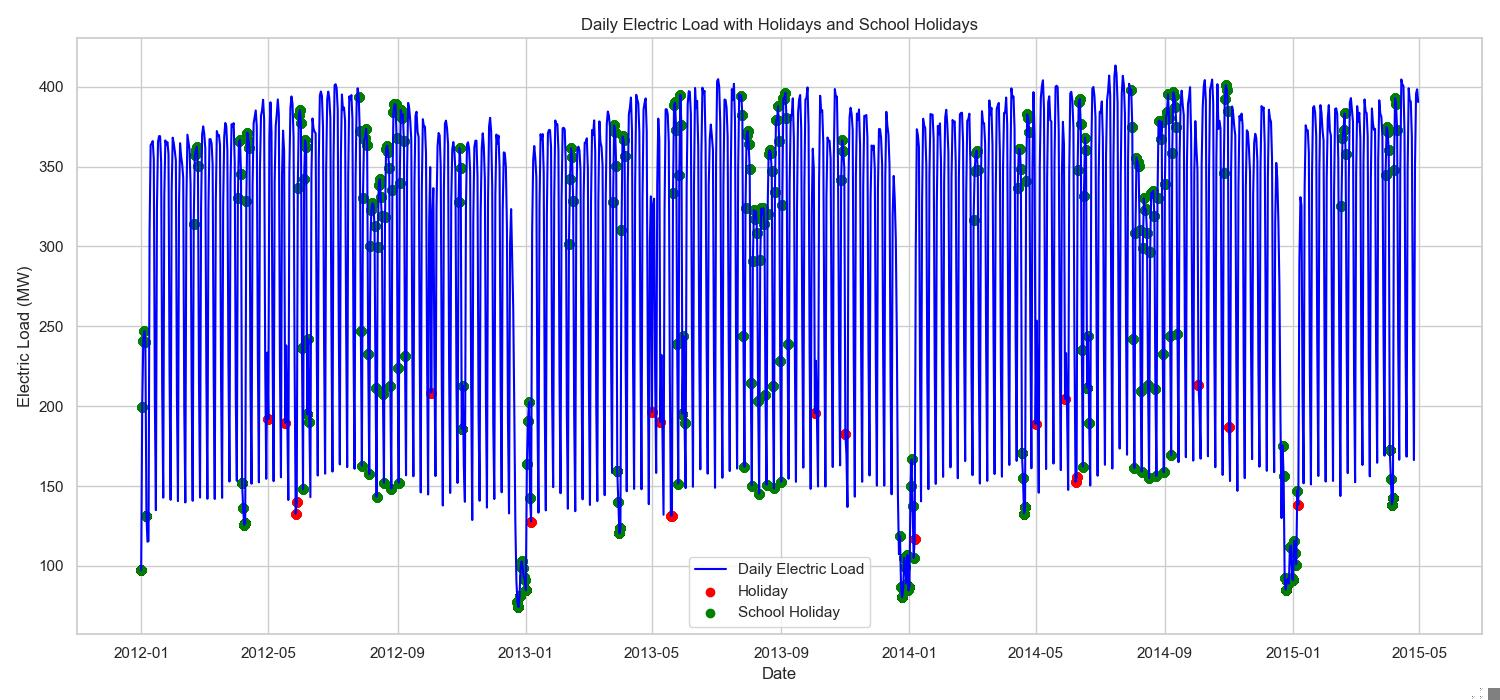
\includegraphics[width=\textwidth]{ressources/Holiday/lectricLoad_holiday.jpg}
        \caption{Load Curve 1}
        \label{fig:RawData1}
    \end{subfigure}
    \\
    \begin{subfigure}[b]{\textwidth}
        \centering
        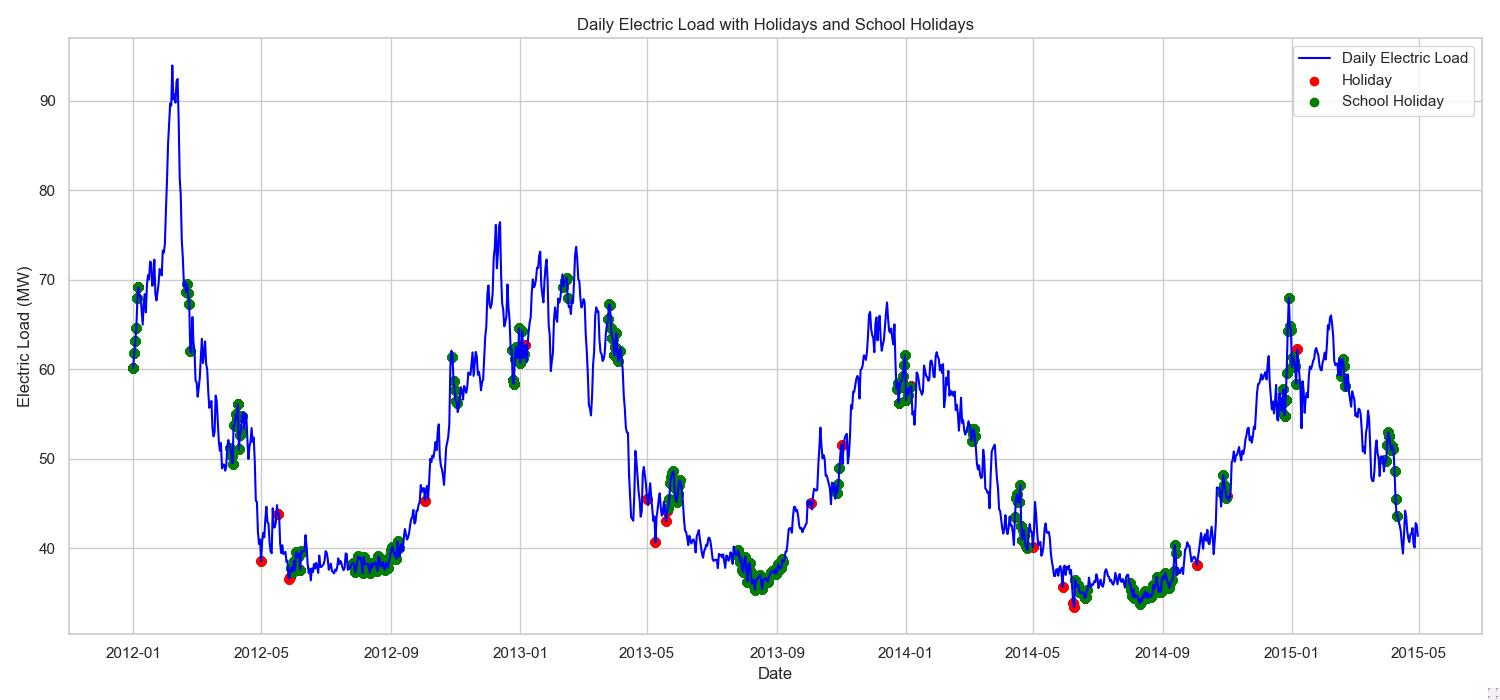
\includegraphics[width=\textwidth]{ressources/Holiday/lectricLoad_holiday(1).jpg}
        \caption{Load Curve 2}
        \label{fig:RawData2}
    \end{subfigure}
    \\
    \begin{subfigure}[b]{\textwidth}
        \centering
        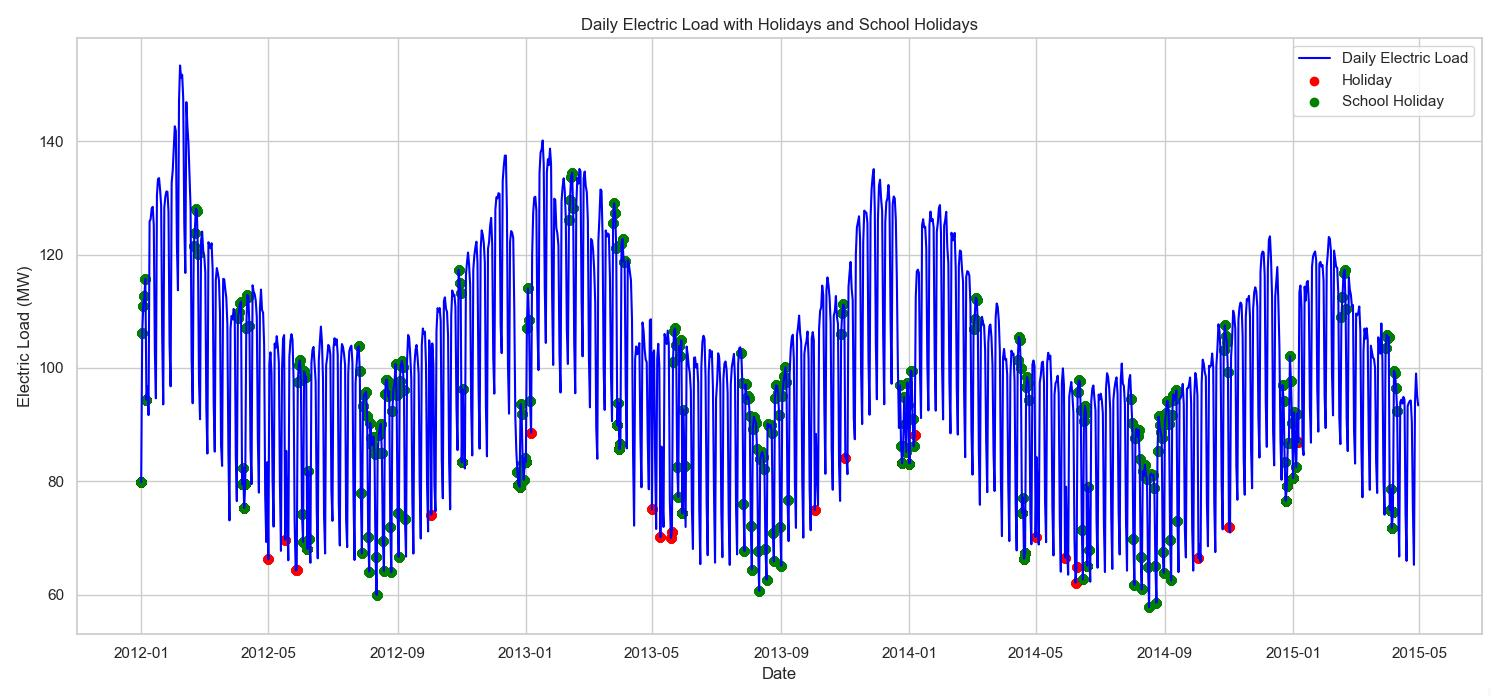
\includegraphics[width=\textwidth]{ressources/Holiday/lectricLoad_holiday(2).jpg}
        \caption{Load Curve 3}
        \label{fig:RawData3}
    \end{subfigure}
    \caption{Load Curves}
    \label{fig:RawData}
\end{figure}

The visual representations in these figures lay out the daily load as a series of vertical blue lines, with the magnitude of each line corresponding to the load on that day. What is particularly evident across all three figures is the occurrence of notable variations during holiday periods, marked in red, and school holidays, marked in green. These markers denote a consistent pattern of reduced load, reflecting the change in electricity consumption that occurs during these times. This consistent pattern across multiple years highlights the impact of these breaks on overall consumption habits. 

To capitalize on these insights, 'Holiday' and 'School Holiday' are identified as features for our forecasting models. These temporal events are encoded as binary features, where a '1' indicates the occurrence of the respective holiday, and a '0' its absence. Incorporating these features allows the models to account for predictable shifts in demand, thus refining the precision of load predictions. 

This feature engineering process illustrates the impact of time-related events on electricity usage, allowing our models to distinguish between regular days and those with unusual load profiles due to holidays. By incorporating 'Holiday' and 'School Holiday' variables into our models, we ensure they are sensitive to the non-linear and temporal factors that affect load patterns. This strategic approach to feature engineering demonstrates our commitment to a data-driven understanding of consumption patterns, which is essential for developing robust predictive models in the complex arena of load forecasting. 

\subsubsection{Integrating Environmental Factors}
The development of characteristics for load forecasts also includes environmental variables such as temperature and radiation, which can have a significant impact on energy consumption. Our dataset includes these variables for some load curves but not for others, presenting an opportunity to assess their correlations with electric load and their potential utility as predictive features. 

For Load Curve One, no temperature or radiation data is available, requiring reliance on other types of features. In contrast, Load Curve Two (Figure \ref{fig:Environmental2}) includes two sets of temperature and radiation readings, and Load Curve Three (Figure \ref{fig:Environmental3}) contains one set of each. The correlation plots provided for these datasets exhibit varying degrees of correlation between these environmental factors and the electric load. Notably, there is a negative correlation between temperature and load in some instances, which could indicate higher temperatures leading to lower electricity usage, possibly due to reduced heating needs. Conversely, positive correlations in certain cases could suggest increased cooling demands during warmer periods. 
\begin{figure}[H]
    \centering
    \begin{subfigure}[b]{\textwidth}
        \centering
        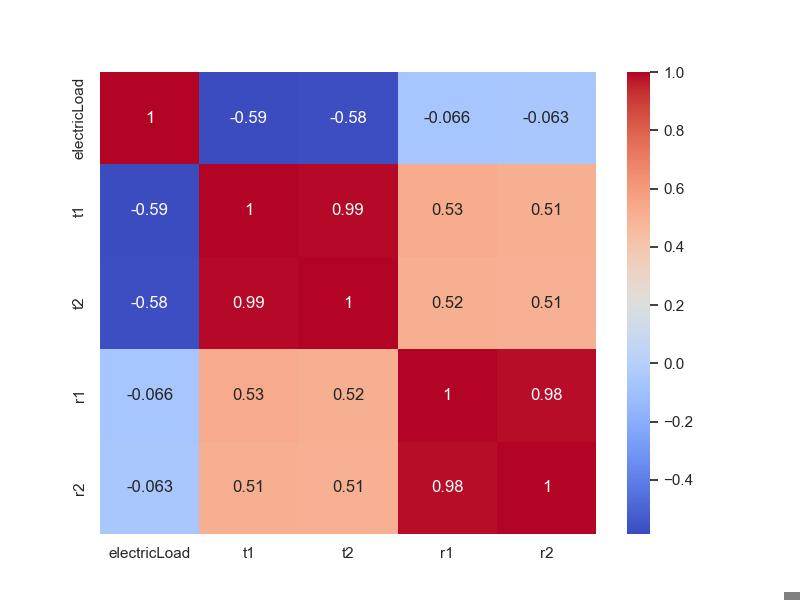
\includegraphics[width=\textwidth]{ressources/Environmental/CorrelationElectricLoadFeatures.jpg}
        \caption{Correlation plot of the environmental factors for Load Curve 2}
        \label{fig:Environmental2}
    \end{subfigure}
    \\
    \begin{subfigure}[b]{\textwidth}
        \centering
        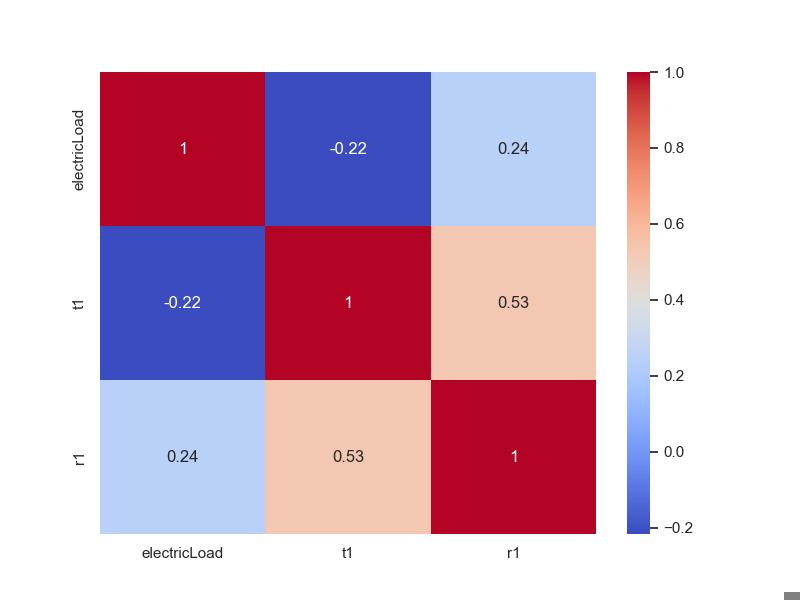
\includegraphics[width=\textwidth]{ressources/Environmental/CorrelationElectricLoadFeatures(1).jpg}
        \caption{Correlation plot of the environmental factors for Load Curve 3}
        \label{fig:Environmental3}
    \end{subfigure}
    \caption{Correlation plot of the environmental factors}
    \label{fig:Environmental}
\end{figure}
Based on these correlation plots, temperature and radiation are added as features to our models for Load Curves Two and Three, where such data is available. It is crucial to acknowledge that these features, like all others, are subject to evaluation during hyperparameter tuning. This process allows us to "switch on" or "off" particular features, determining their influence on the model's performance. Through hyperparameter tuning, we can identify the most predictive features, ensuring that only those that contribute positively to the accuracy of the forecasts are retained. 

This flexible approach to feature inclusion ensures that our models remain adaptable and are fine-tuned to the specifics of the data they are trained on. By dynamically selecting features during the tuning process, we can build models that are both robust and sensitive to the nuances of environmental impacts on electric load, ultimately improving the precision and reliability of our load forecasting efforts. 

\subsubsection{Daylight Phase and Day of Week }
As we delve deeper into the nuances of feature engineering for load forecasting, the incorporation of temporal elements is crucial. Our analysis includes the introduction of sophisticated time-related features, such as the phase of daylight and the day of the week, both of which are depicted in Figure 9, Figure 10 and Figure 11. These figures provide a heatmap representation of the average electric load across different daylight phases and days of the week, presenting an average over three separate years. 

The function \texttt{get\_daylight\_phase(row)} is instrumental in our feature engineering, calculating the time of day in relation to sunrise and sunset. By using this function, we classify each timestamp into one of five categories: 

\begin{itemize}
    \item pre-dawn (0)
    \item post-dawn/pre-noon (1)
    \item post-noon/pre-sunset (2)
    \item post-sunset (3)
    \item night (4).
\end{itemize}


This categorization captures the variation in electric load as it correlates with natural light, acknowledging that human activity, and consequently energy usage, aligns with these daily transitions. In addition to the daylight phase, the day of the week is another pivotal feature. Behavioral patterns differ significantly between weekdays and weekends, affecting energy consumption trends. This differentiation is crucial for anticipating weekly cycles in load patterns. 

Figure \ref{fig:Daylight} illustrates these relationships, with varying load intensities highlighted by color gradients. Higher loads are noticeable during certain daylight phases, indicating peak consumption periods. The variation by day of the week is also apparent, with weekdays generally showing higher consumption levels compared to weekends. This visualization provides a clear indication of how both daylight phase and day of the week influence the electric load, justifying their inclusion as features in our forecasting models. 

By integrating "Daylight Phase" and "Day of Week" into our models, we aim to capture the cyclical nature of electric load. The strategic inclusion of these features, grounded in the empirical evidence from our visual analysis, allows our models to adjust predictions according to the time-based patterns observed, enhancing the accuracy and reliability of our load forecasts. Feature engineering demonstrates our commitment to a data-driven understanding of consumption patterns, which is essential for developing robust predictive models in the complex arena of load forecasting. 

\begin{figure}[H]
    \centering
    \begin{subfigure}[b]{0.7\textwidth}
        \centering
        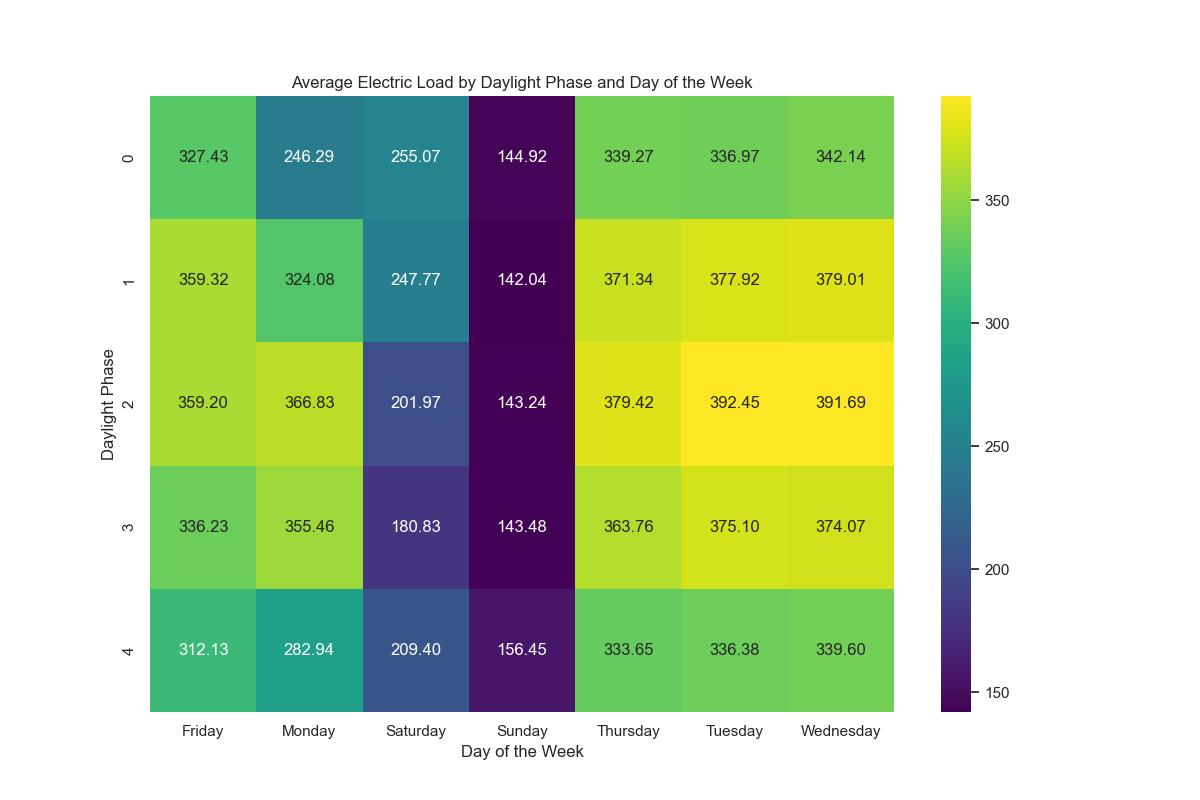
\includegraphics[width=\textwidth]{ressources/Daylight_Week/ElectricLoadDaylight(1).jpg}
        \caption{Electric Load by Daylight Phase and Day of Week of Load Curve 1}
        \label{fig:Daylight1}
    \end{subfigure}
    \\
    \begin{subfigure}[b]{0.7\textwidth}
        \centering
        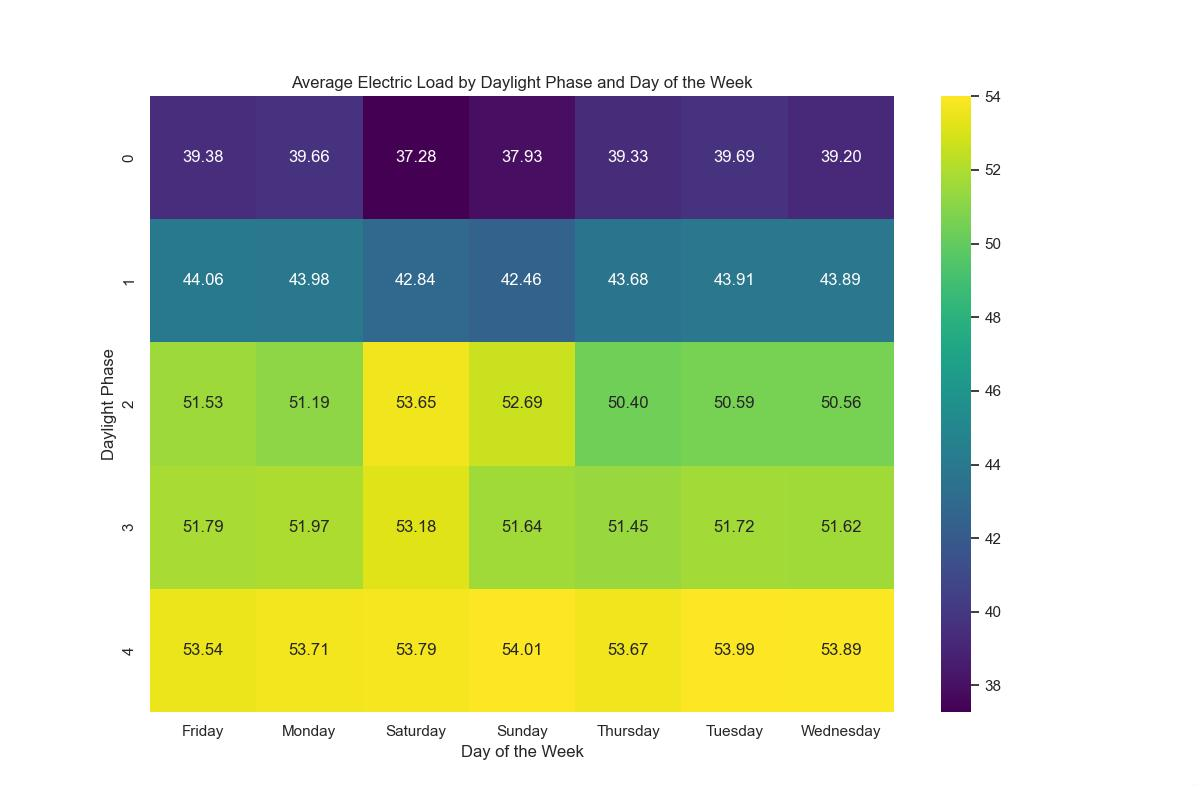
\includegraphics[width=\textwidth]{ressources/Daylight_Week/ElectricLoadDaylight(2).jpg}
        \caption{Electric Load by Daylight Phase and Day of Week of Load Curve 2}
        \label{fig:Daylight2}
    \end{subfigure}
    \\
    \begin{subfigure}[b]{0.7\textwidth}
        \centering
        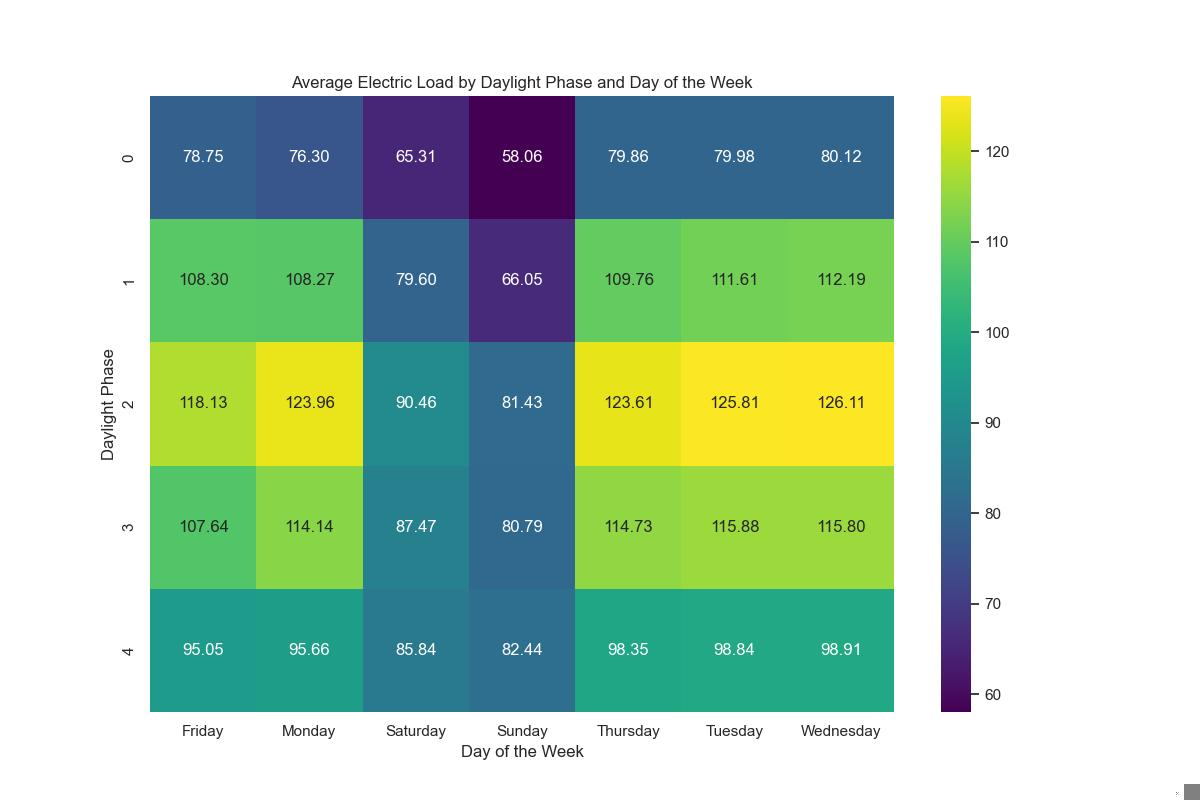
\includegraphics[width=\textwidth]{ressources/Daylight_Week/ElectricLoadDaylight(3).jpg}
        \caption{Electric Load by Daylight Phase and Day of Week of Load Curve 3}
        \label{fig:Daylight3}
    \end{subfigure}
    \caption{Average Electric Load by Daylight Phase and Day of Week}
    \label{fig:Daylight}
\end{figure}



\subsubsection{Autocorrelation Insights}
In our pursuit of precision within the realm of load forecasting, we pay particular attention to the role of autocorrelation revealed in the time series data of electric load. The autocorrelation plots provide a window into the relationship between the electricity load and its past values, showcasing how historical data can inform future predictions. This temporal linkage is depicted in the fluctuations of the autocorrelation coefficient over various lag periods, suggesting a patterned dependency that is cyclic and seasonal in nature. 

While the Figure \ref{fig:autocorrelation} clearly indicate the presence of seasonality, the specific drivers behind these patterns are not immediately apparent. A deeper understanding of the context—such as local climate conditions, industrial operational schedules, or communal events—could unveil the factors that influence these autocorrelations. Identifying the exact causes of the observed seasonal trends would empower us to engineer more sophisticated features, such as indicators for local festivities or temperature adjustments that account for climate impact on energy consumption. 

Within the framework of our feature engineering, we also employ a sliding window technique, a powerful method for capturing temporal dependencies and trends within time series data. This approach involves creating features based on the values from preceding time steps, effectively sliding a window across the data to construct a sequence of lagged observations. By systematically shifting this window and capturing the corresponding subsets of data, we create a structured representation of the time series that reflects its historical values. 

The sliding window encapsulates a specified number of past and future time steps, allowing the model to learn from the sequence of recent loads when predicting future demand. This methodology not only captures the inherent autocorrelation observed in the plots but also provides the model with a richer set of input features that include the immediate historical context. 

Implementing a sliding window is particularly beneficial in situations where past load patterns are indicative of future behavior, a common characteristic in energy consumption data. It is a dynamic and adaptable technique, where the window size can be tuned to the specific periodicity and seasonality inherent in the dataset, ensuring that the generated features are optimally aligned with the forecasting objectives.  

This reflection on autocorrelation not only guides our current feature engineering efforts but also paves the way for ongoing refinement. As our understanding of the specific application case deepens, our feature engineering process will evolve, continually improving the predictive power of our load forecasting models. This iterative enhancement is central to our methodology, underscoring our commitment to developing models that are as informative and reliable as the rich datasets they learn from. 
\begin{figure}[H]
    \centering
    \begin{subfigure}[b]{\textwidth}
        \centering
        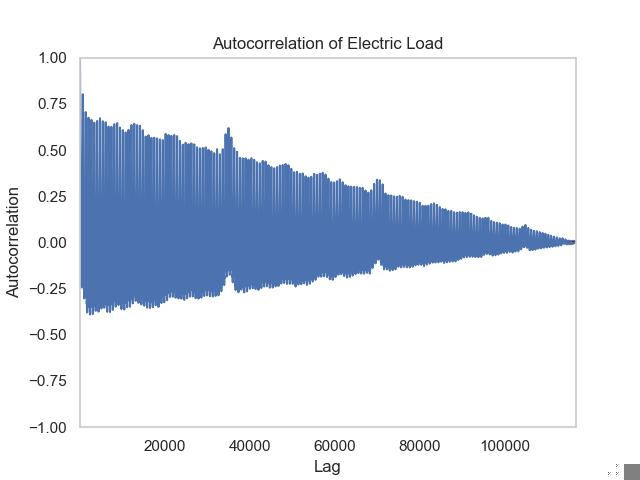
\includegraphics[width=0.65\textwidth]{ressources/Autocorrelation/lectricLoad_autocorrelation.jpg}
        \caption{Autocorelation of Load Curve 1}
        \label{fig:autocorrelation1}
    \end{subfigure}
    \\
    \begin{subfigure}[b]{\textwidth}
        \centering
        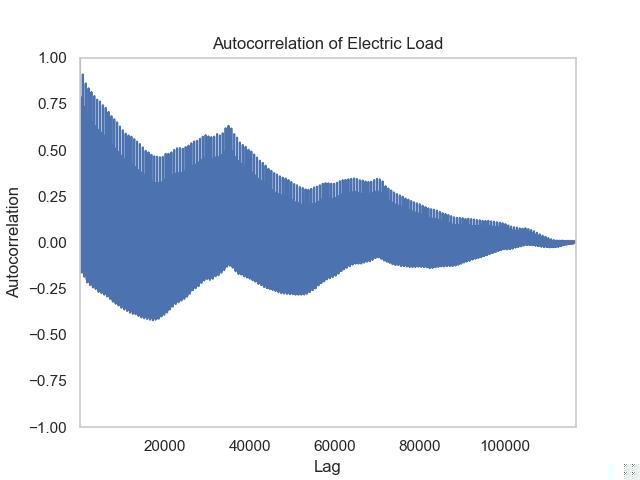
\includegraphics[width=0.65\textwidth]{ressources/Autocorrelation/lectricLoad_autocorrelation(1).jpg}
        \caption{Autocorelation of Load Curve 2}
        \label{fig:autocorrelation2}
    \end{subfigure}
    \\
    \begin{subfigure}[b]{\textwidth}
        \centering
        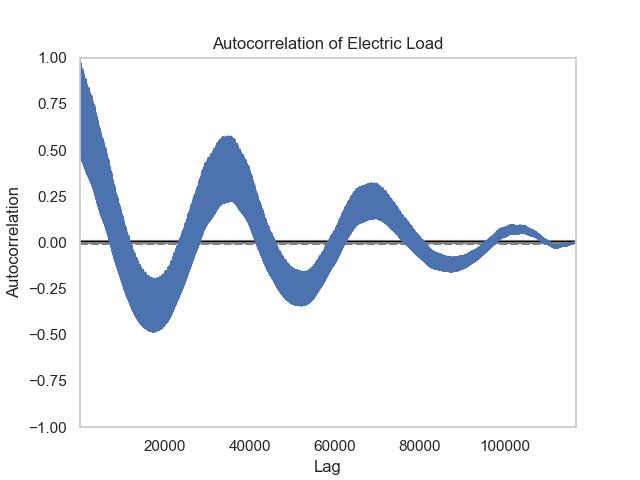
\includegraphics[width=0.65\textwidth]{ressources/Autocorrelation/lectricLoad_autocorrelation(2).jpg}
        \caption{Autocorelation of Load Curve 3}
        \label{fig:autocorrelation3}
    \end{subfigure}
    \caption{Autocorelation}
    \label{fig:autocorrelation}
\end{figure}


\subsection{Model Development and Training}
In the subsequent sections, we detail the program flow underlying our predictive modelling efforts, which is fundamentally divided into two main stages as depicted in Figure \ref{fig.:flowChart}. This flow is designed to optimize our models for precision in electric load forecasting. 
\begin{figure}[h]
\begin{center}
%\framebox[4.0in]{$\;$}
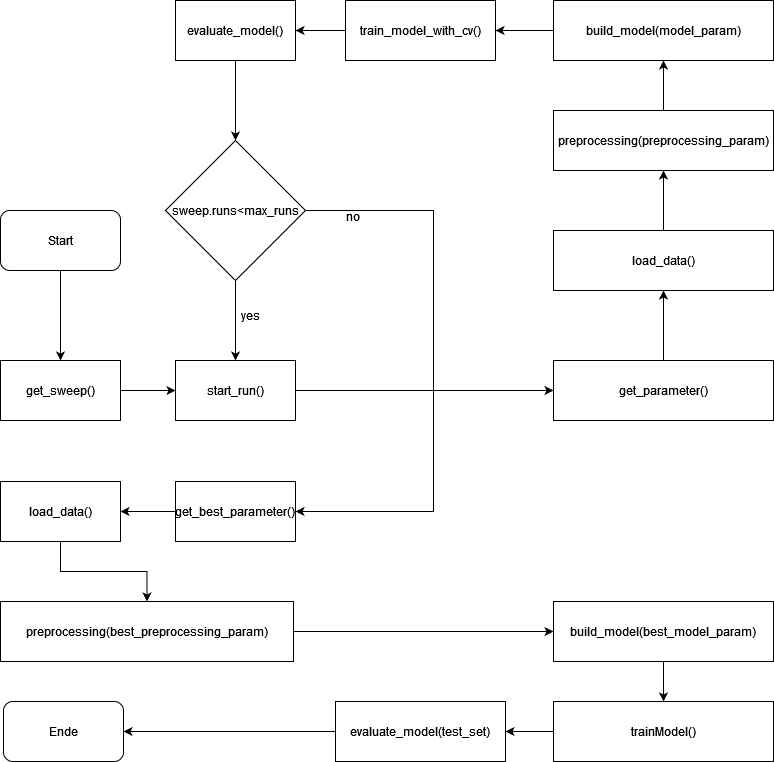
\includegraphics[width=\textwidth]{ressources/CSOAII.drawio(1).png}
\end{center}
\caption{Flow chart of the program execution}
\label{fig.:flowChart}
\end{figure}

The initial stage centers around hyperparameter optimization, where Bayesian optimization techniques are applied to fine-tune the model parameters. This process is augmented with cross-validation to ensure that the selected hyperparameters generalize well to unseen data, thereby enhancing the robustness of the models. 

Following the optimization, the best-performing model parameters are utilized to conduct the final training. This definitive step is crucial as it consolidates the insights gained from the optimization process and aligns the model with the intricacies of the dataset. 

The training procedure initiates with the creation of a \gls*{WandB} project session. \gls*{WandB} serves as an experiment tracking platform, enabling us to systematically log and monitor various metrics and configurations throughout the training process. Each training run is timestamped and recorded, facilitating the comparison of model performances and configurations over time. 

The next step involves reading the dataset from a CSV file and applying a series of preprocessing operations. These operations are designed to prepare the data for training, encompassing data cleaning, feature engineering, and splitting into training, validation, and test sets. The preprocessing parameters are dynamically adjusted based on the configuration, providing the flexibility to explore various preprocessing strategies and assess their impact on model performance. Detailed descriptions of the feature generation process, including the specific strategies and techniques employed, are provided in Section \ref{subCha.:FeatureGeneration}, "Feature Generation". This section delves into the intricacies of how features are engineered and parameterized, illustrating our methodical approach to enhancing the predictive capabilities of our models. 

The core of our hyperparameter tuning process employs \gls*{CV}, a technique that ensures the robustness and generalizability of our models. The \gls*{CV} process iterates over a predefined grid of hyperparameters, assessing each combination's performance to pinpoint the most effective configuration. Upon concluding the \gls*{CV} phase, we aggregate and log the performance metrics of each fold in \gls*{WandB}, providing a granular view of the model's performance across different subsets of the data. This detailed logging aids in understanding the model's consistency and the reliability of its predictive accuracy. 

Hyperparameters and data preprocessing parameters are loaded from either a YAML configuration file or a \gls*{WandB} sweep configuration, depending on their role in the training process. Static parameters, which remain unchanged across experiments, are specified in the YAML file. This ensures a stable base for each model training session, providing consistency and traceability for fundamental aspects of the model and preprocessing setup. Conversely, parameters subject to optimization are defined within the \gls*{WandB} sweep configuration. This delineation allows for dynamic adjustment and systematic exploration of the hyperparameter space, facilitating the identification of optimal model configurations through automated sweeps. The separation of static and optimizable parameters into YAML and sweep configurations, respectively, enhances the flexibility and efficiency of our experimentation, enabling targeted optimizations that are crucial for advancing the performance of our forecasting models. 
Following the determination of the best hyperparameters, the model is trained on the combined training and validation datasets. This final training step is crucial for leveraging the full breadth of available data, further refining the model's ability to generalize to unseen data. The training process incorporates callbacks for real-time monitoring and logging in \gls*{WandB}, offering insights into the model's learning progression. 

Once the training is complete, the model is saved to a specified path, and a final evaluation is conducted. This evaluation assesses the model's performance on the test dataset, utilizing metrics such as Huber loss, to quantify its predictive accuracy and error characteristics. The evaluation results are critical for understanding the model's practical applicability and forecasting prowess. 

\subsection{Model Specific Characteristics}

In this section, we delve into the specifics of the models employed in our study, each chosen for its unique capabilities in addressing the complexities of load forecasting. 


\subsubsection{XGBoost}
\Gls*{xgboost} stands as a sophisticated ensemble learning algorithm renowned for its performance and speed. Our implementation leverages a series of decision trees constructed in a gradient boosting framework. Specific parameters such as "learning\_rate", "max\_depth", and "colsample\_bytree" were fine-tuned to optimize the model's ability to capture complex non-linear patterns within the load forecasting data. The use of regularization parameters, "reg\_alpha" and "reg\_lambda", was instrumental in controlling overfitting, thereby ensuring the model's robustness. Model training included an evaluation phase using a validation set, with the "WandbCallback" ensuring real-time monitoring and logging within \gls*{WandB}.
One of the key strengths of XGBoost is its flexibility in handling different types of loss functions, including Pseudo Huber loss, which is particularly useful for regression tasks. Huber loss is chosen for its robustness to outliers, as it combines the advantages of L1 loss (least absolute deviations) and L2 loss (least squares). For errors smaller than a threshold, Huber loss behaves like L2 loss, which is sensitive to small errors but gives a quadratic penalty to them. For errors larger than the threshold, it behaves like L1 loss, which is less sensitive to large errors and provides a linear penalty. This hybrid approach allows XGBoost to minimize the impact of outliers on the model's performance, leading to more accurate and reliable predictions, especially in scenarios where the data contains many outliers or is highly skewed \cite{kulisz2024optimizing}.

\subsubsection{ARD}
The \gls*{ARD} Regression model is particularly notable for its capacity to determine the relevance of features within the dataset. By applying a Bayesian framework to linear regression, \gls*{ARD} can effectively shrink coefficients for less relevant features to zero, simplifying the model and potentially preventing overfitting. Parameters such as "alpha\_1", "alpha\_2", "lambda\_1", and "lambda\_2" control the shape and scale of the prior distributions over the weights, influencing the model's complexity and adaptability. 


\subsubsection{KNN}
The \gls*{KNN} is an instance-based learning model that predicts the target variable's value based on the weighted average of the k-nearest neighbors. It is inherently non-parametric and can capture complex local structures in data. The distance metric, the "leaf\_size", the power parameter for the Minkowski metric. The number of neighbors ("n\_neighbors") were key hyperparameters optimized in our study.  
The Minkowski metric is a generalized distance metric that encompasses both Euclidean and Manhattan distances as special cases. It is defined as $(\sum_{i=1}^{n} |x_i - y_i|^p)^{1/p}$, where $x$ and $y$ are two points in an $n$-dimensional space, and $p$ is the power parameter. When $p=2$, the Minkowski metric becomes the Euclidean distance, which measures the shortest path between two points. When $p=1$, it becomes the Manhattan (or city block) distance, which measures the sum of the absolute differences of their Cartesian coordinates. The choice of $p$ allows for flexibility in how distance is calculated, influencing the behavior of the KNN algorithm. By optimizing the power parameter for the Minkowski metric in our study, we aimed to find the most suitable way to measure distances between instances, thereby improving the model's prediction accuracy \cite{bishop2006pattern}.

\subsubsection{LSTM}
The \gls*{LSTM} network is applied to model time-series dependencies in load forecasting. Due to its recurrent nature, it is capable of learning from the long-term temporal sequence of the data, an essential feature given the time-series nature of load curves. Our model employs bidirectional LSTMs to capture patterns across different time scales effectively and is complemented by dropout layers to mitigate overfitting. An exponential decay learning rate schedule is utilized to fine-tune the training process dynamically. 
For the \gls*{LSTM} model, the Huber loss function is chosen for its resilience to outliers, reducing the impact of rare but large errors on the overall model performance. 

\subsection{Evaluation}
Our methodology extends into a thorough evaluation framework, ensuring our models robustness and accuracy in forecasting loads.
Hyperparameter optimization is conducted using the \gls*{MSE} metric, which quantifies the average of the squares of the errors or deviations. 

Upon finalizing the training, our models are evaluated through a bespoke function, \texttt{evaluate\_model()}, which assesses model predictions against actual labels using a suite of metrics. This function calculates \gls*{MSE}, \gls*{RMSE}, \gls*{MAE}, and the \gls*{R2} for both test and, if available, validation datasets. These metrics collectively provide a nuanced view of model performance, encompassing error magnitude, prediction accuracy, and the proportion of variance explained by the model. The inclusion of variance in residuals as a logged metric offers insights into prediction consistency and reliability. 

Crucially, our evaluation process is integrated with \gls*{WandB}, allowing us to log all metrics and training parameters. This not only facilitates real-time monitoring and comparison of model performance but also ensures the reproducibility of our results. Through \gls*{WandB}, stakeholders can easily trace the experimental setups leading to the reported outcomes, fostering transparency and facilitating future research endeavors. 

By adopting cross-validation early in our model training process, we ensure that our models are not only tuned for optimal performance but also tested for their generalization capability across unseen data. This methodical approach, from data partitioning and hyperparameter optimization to comprehensive model evaluation. 

\section{Business Insights}
Our analysis of the predictive model has unveiled several key business insights; however, further contextual details are essential for a comprehensive interpretation. Understanding the specific machinery involved, such as whether it pertains to a Nuclear Power Plant or other industrial contexts, is crucial for refining the model's applicability and relevance. One notable observation is the presence of strong seasonality in the load curves. While the exact source of this seasonality requires additional context, it likely stems from production cycles or other operational patterns inherent to the machinery. Incorporating this contextual information as a feature in our model could significantly enhance its precision, allowing for more accurate load predictions.

Overall, our model demonstrates high precision in load prediction, offering valuable opportunities for business exploitation. For instance, the ability to accurately forecast load curves enables organizations to strategically capitalize on fluctuations in energy prices. By utilizing our model's insights, businesses can optimize energy consumption patterns to minimize costs during periods of high energy prices and capitalize on opportunities for cost savings during periods of low energy prices. Furthermore, there is potential for further refinement. Access to additional environmental data, such as temperature and radiation levels, or the integration of more sensors on the machinery, could enhance feature engineering and unlock deeper insights. With a more extensive dataset and advanced feature engineering techniques, our model could provide even more nuanced insights for optimizing energy management strategies. By incorporating contextual information, refining feature engineering, and exploring additional environmental data sources, we can unlock even greater insights and opportunities for strategic decision-making in energy management.

\section{Results}
In the results section of this study, we systematically evaluate the performance of four distinct predictive models, each scrutinized individually to understand their efficacy and characteristics in the context of our dataset. Initially, we delve into \gls*{xgboost}, which, as preliminary analyses suggest, stands out for its superior predictive accuracy and efficiency. Following \gls*{xgboost}, we explore \gls*{ARD}, then proceed to examine \gls*{KNN}, and finally, assess the capabilities of \gls*{LSTM}. Our focus predominantly lies on \gls*{xgboost} due to its exceptional performance across various metrics, positioning it as the most promising model among those evaluated. The culmination of this section presents a comparative analysis of all models, aiming to provide a comprehensive overview of their relative strengths and weaknesses in the pursuit of optimizing predictive performance. 

\subsection{XGBoost}

\subsubsection{Analysis of Bayesian Hyperparameter Optimization for XGBoost}
This section presents an analysis of the Bayesian hyperparameter optimization process for the XGBoost algorithm, focusing on Load Curves 1, 2, and 3. We discuss the trends and implications of the cross-validation Mean Squared Error across 30 evaluation runs.

For Load Curve 1, the optimization process showed an initial decrease in \texttt{MSE}, indicating rapid improvements in model configuration, shown in Figure \ref{fig:xgboost_lc1}. Each point reflects the result of a run. The average MSE of the cross validation is plotted on the y axis. The light blue line is the smallest MSE at the time. This description applies to all MSE trend plots. After the initial gains, the reduction in \texttt{MSE} continued at a slower pace, suggesting that the optimization was approaching an optimal set of hyperparameters. The lowest \texttt{MSE} achieved offers an indication of the model's capability to generalize well to unseen data when using the most favorable hyperparameters discovered during the optimization, with the lowest MSE being 643.4. 
\begin{figure}[H]
    \centering
    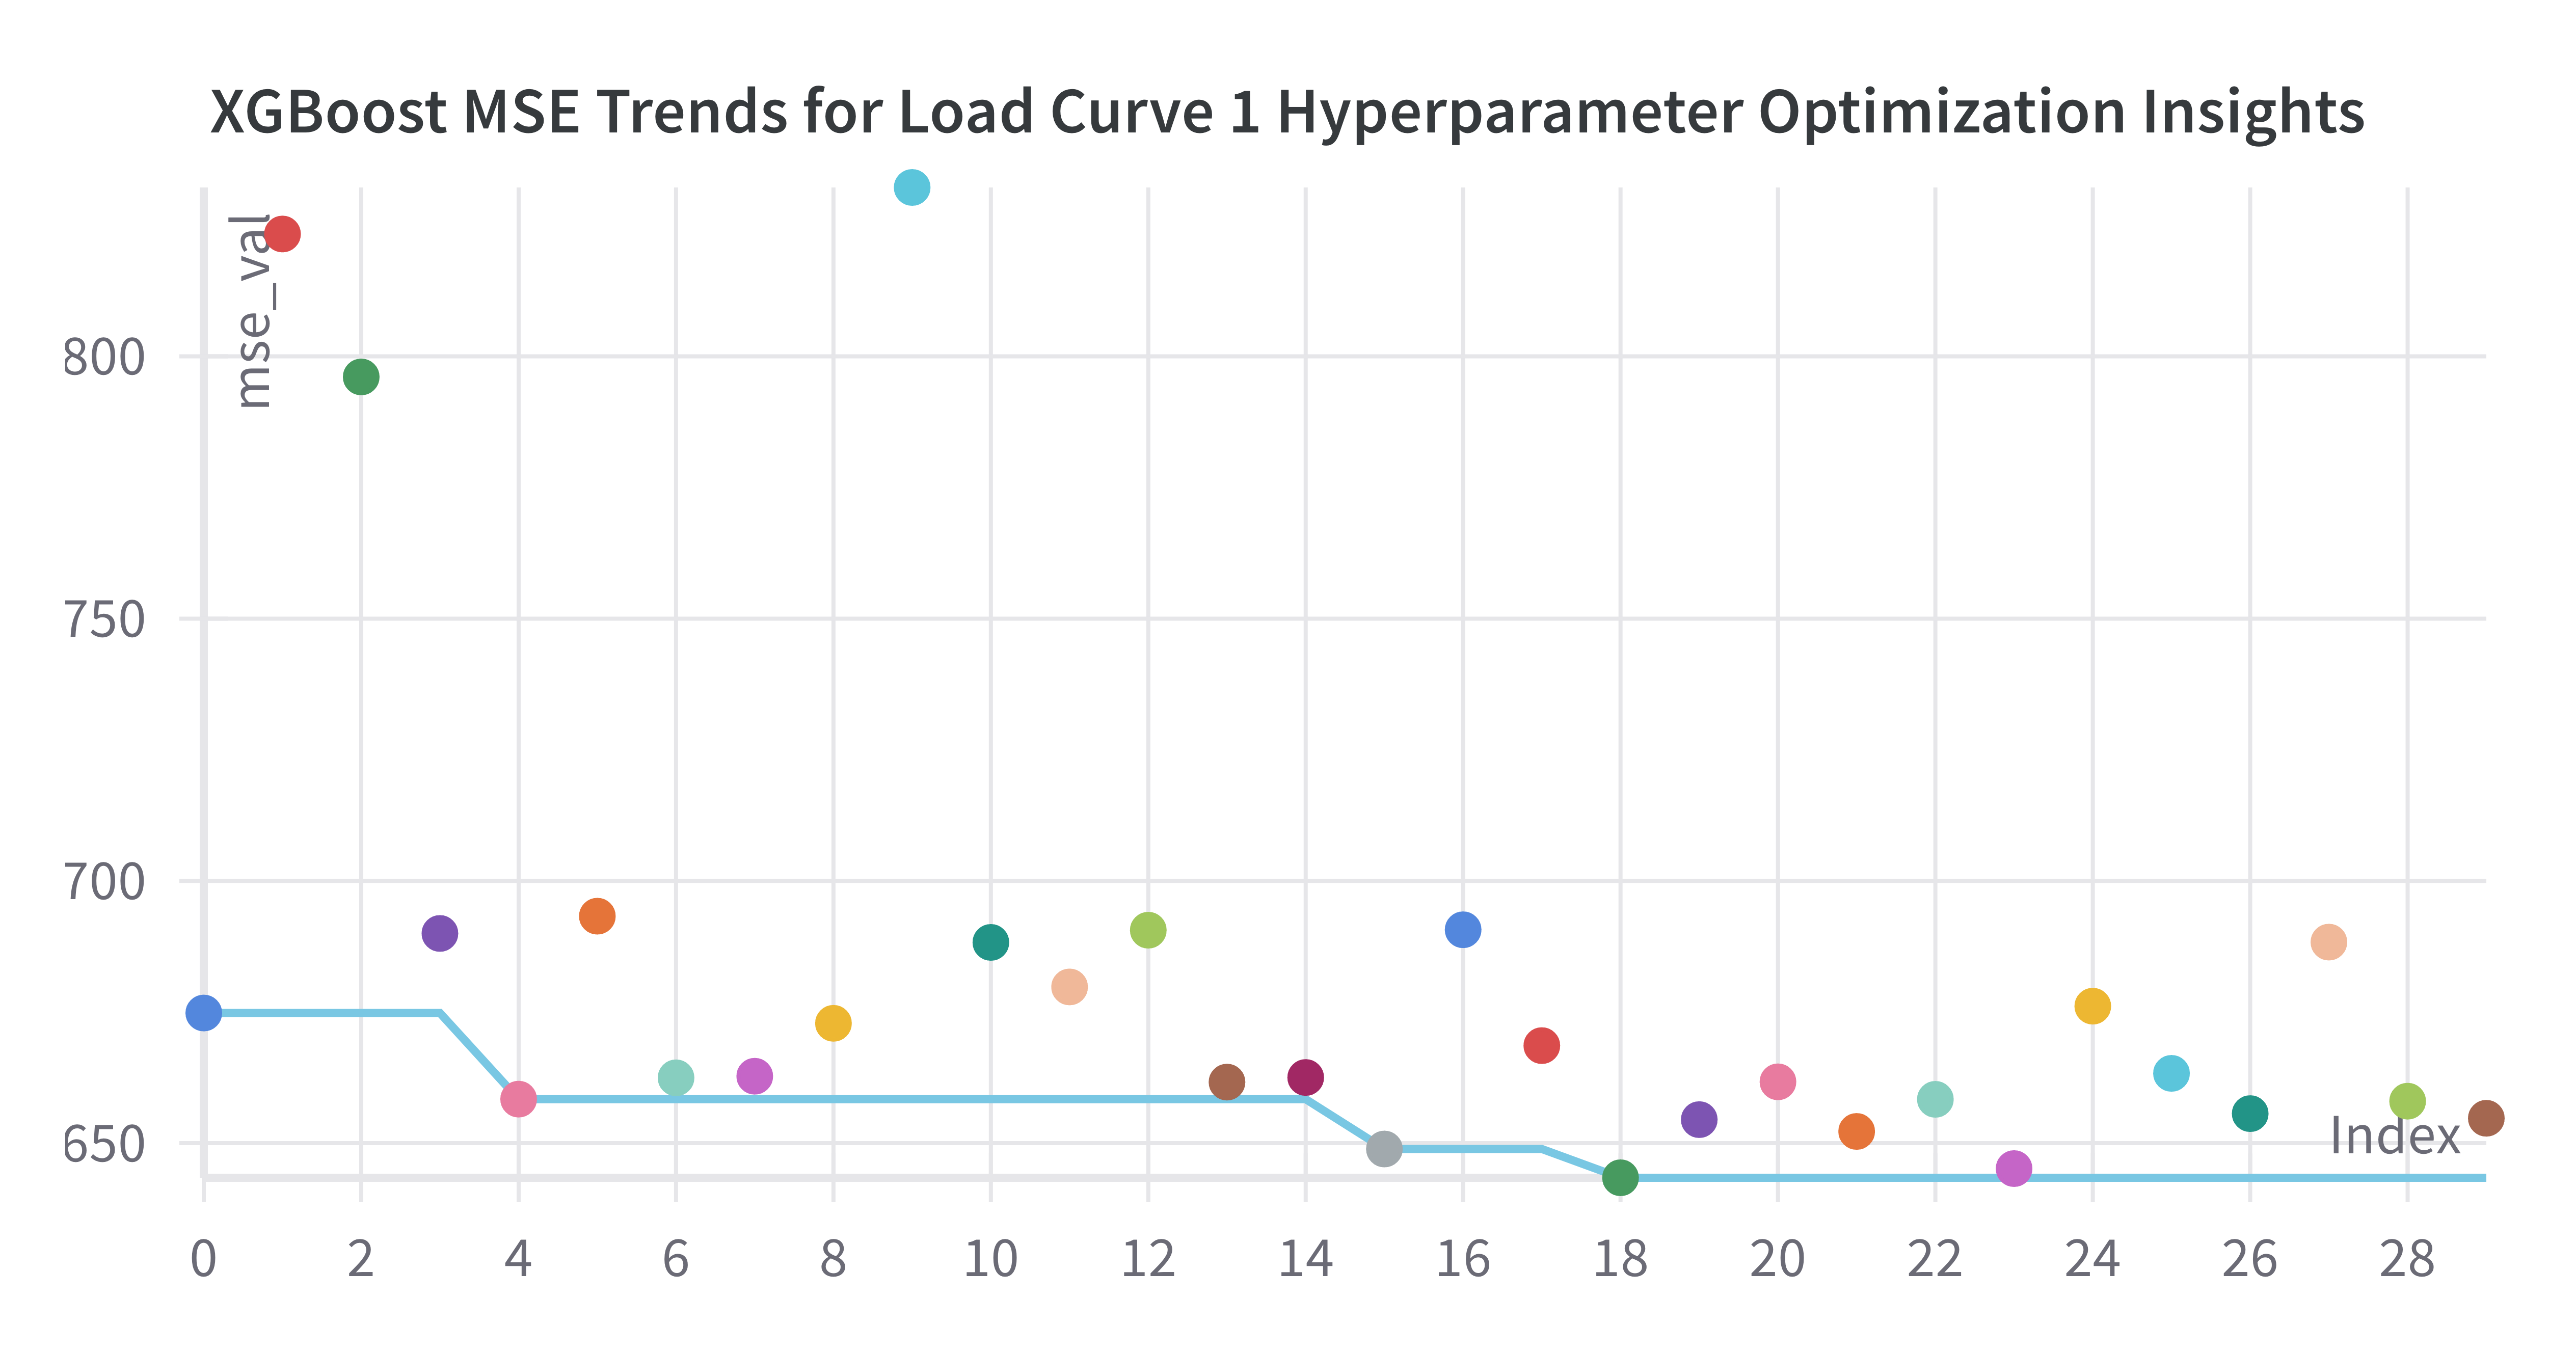
\includegraphics[width=0.75\textwidth]{ressources/Hyperparams/XGBoost/XGBoost MSE Trends for Load Curve 1 Hyperparameter Optimization Insights.png}
    \caption{Bayesian hyperparameter optimization trends for XGBoost on Load Curve 1.}
    \label{fig:xgboost_lc1}
\end{figure}
The most negatively correlated parameter with the target variable is \texttt{max\_depth}, suggesting that deeper trees tend to reduce error, likely due to a better capture of complex patterns. Conversely, \texttt{subsample} shows a negative correlation, indicating that higher subsample rates may benefit the model performance, likely due to reduced overfitting. The \texttt{reg\_lambda} also has a notable positive correlation, implying that the model needs more regularisation.

In the best configurations, parameters like \texttt{max\_depth} at 10, \texttt{subsample} at 0.425, and \texttt{reg\_alpha} at 1.941 align with the correlations observed, indicating a tuned balance between model complexity and regularisation.

The trend for load curve 2 shows a gradual decrease with occasional increases, reflecting the trade-off between exploration and exploitation inherent in Bayesian optimization. This is illustrated in Figure \ref{fig:xgboost_lc2}. The variability of \texttt{MSE} values at certain points indicates that certain hyperparameter combinations were less effective, highlighting the stochastic nature of the process. Nevertheless, a combination of hyperparameters was found which resulted in a \texttt{MSE} value of 8.455.

The \texttt{max\_depth} stands out with the highest correlation of 0.411, which is in line with the need to control model complexity. The \texttt{reg\_lambda} with a correlation of -0.159 shows the effect of L2 regularization in controlling the model complexity. The negative correlation of \texttt{subsample} at 0.202 further supports the model's need for randomness to improve performance.

Load Curve 2's best configuration reflects a depth of 6, with \texttt{subsample} of 0.842 and \texttt{reg\_alpha} at 1.533, suggesting a model that leverages almost the full dataset with regularization to maintain robustness.
\begin{figure}[H]
    \centering
    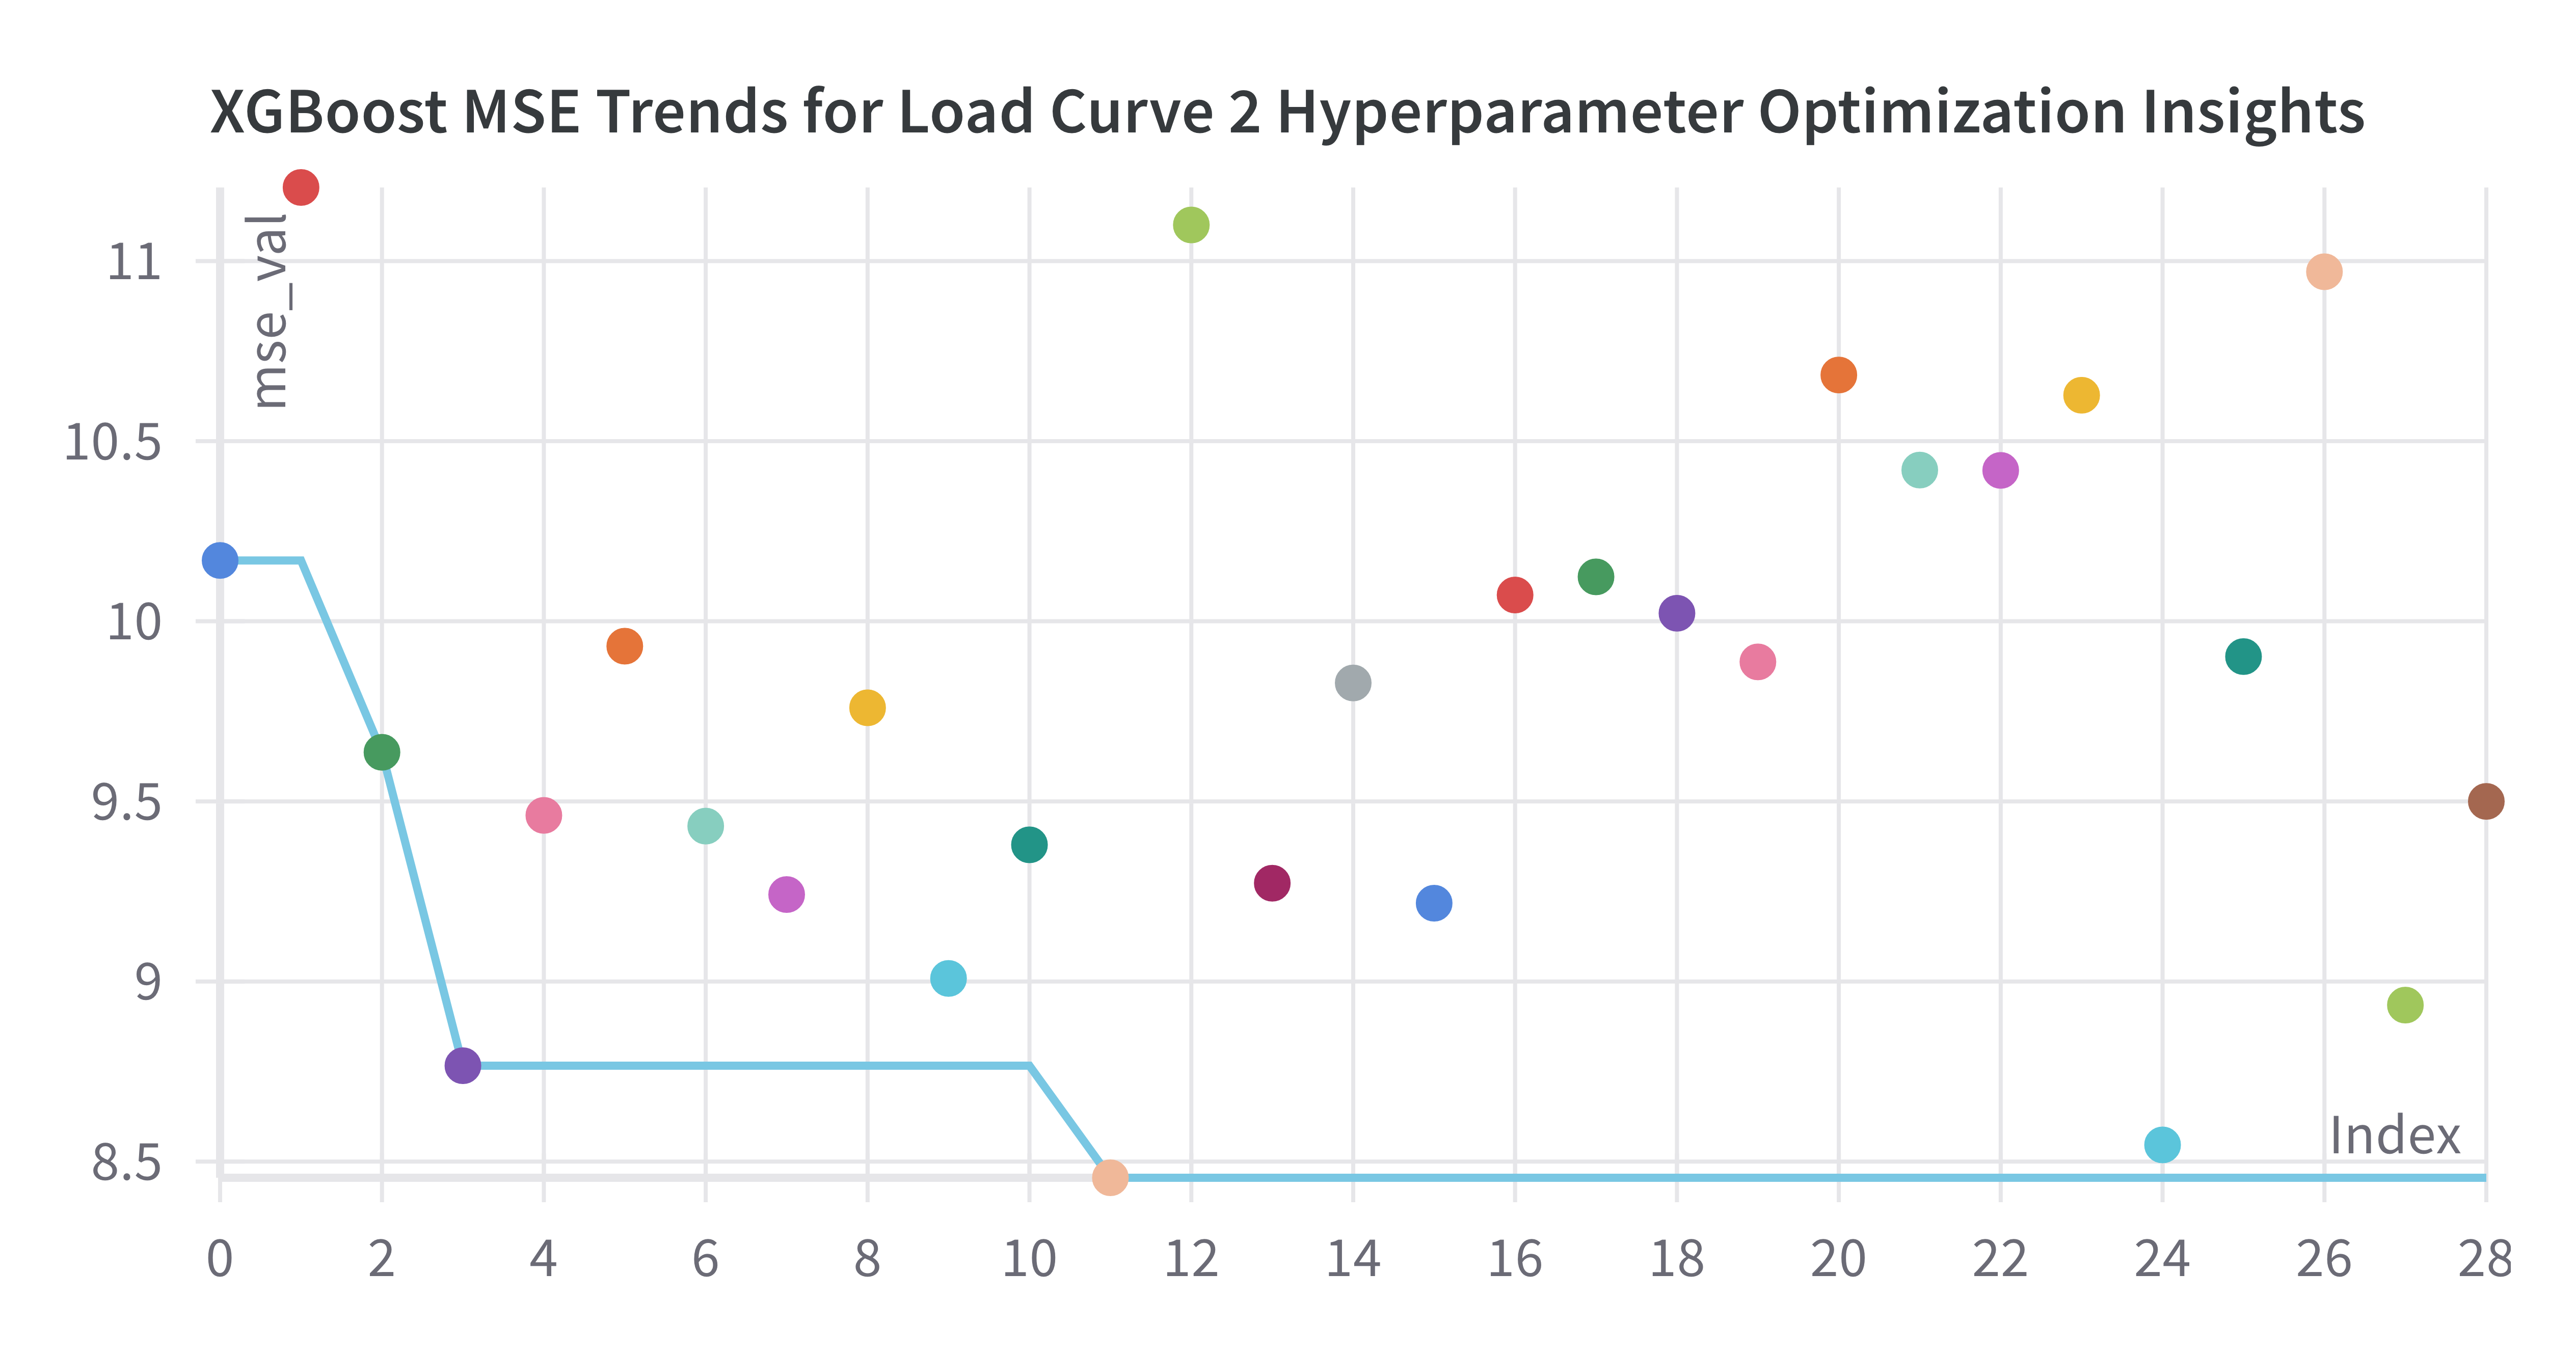
\includegraphics[width=0.75\textwidth]{ressources/Hyperparams/XGBoost/XGBoost MSE Trends for Load Curve 2 Hyperparameter Optimization Insights.png}
    \caption{Bayesian hyperparameter optimization trends for XGBoost on Load Curve 2.}
    \label{fig:xgboost_lc2}
\end{figure}
The \texttt{MSE} for Load Curve 3 depicts a rapid initial improvement. This is shown in Figure \ref{fig:xgboost_lc3}. Nevertheless, there is still a high degree of variance. In spite of this, at the end of the hyperparameter optimization process, even better values of these parameters could be found. The lowest \texttt{MSE} is 29.199.

Similarly, \texttt{max\_depth} has a strong negative correlation of -0.606, emphasizing careful calibration to avoid overfitting. The \texttt{colsample\_bytree} value has a substantial negative correlation of -0.569, again highlighting the need for introducing stochasticity into the model training process. The correlation of \texttt{min\_child\_weight} at 0.324 shows the influence of the regularization parameters on model performance, indicating the importance of penalizing model complexity to improve prediction performance.

For Load Curve 3, the best configuration with \texttt{max\_depth} at 8, \texttt{subsample} at 0.104, and \texttt{reg\_alpha} at 0.987 confirms the importance of these parameters in achieving optimal forecasting performance.
\begin{figure}[H]
    \centering
    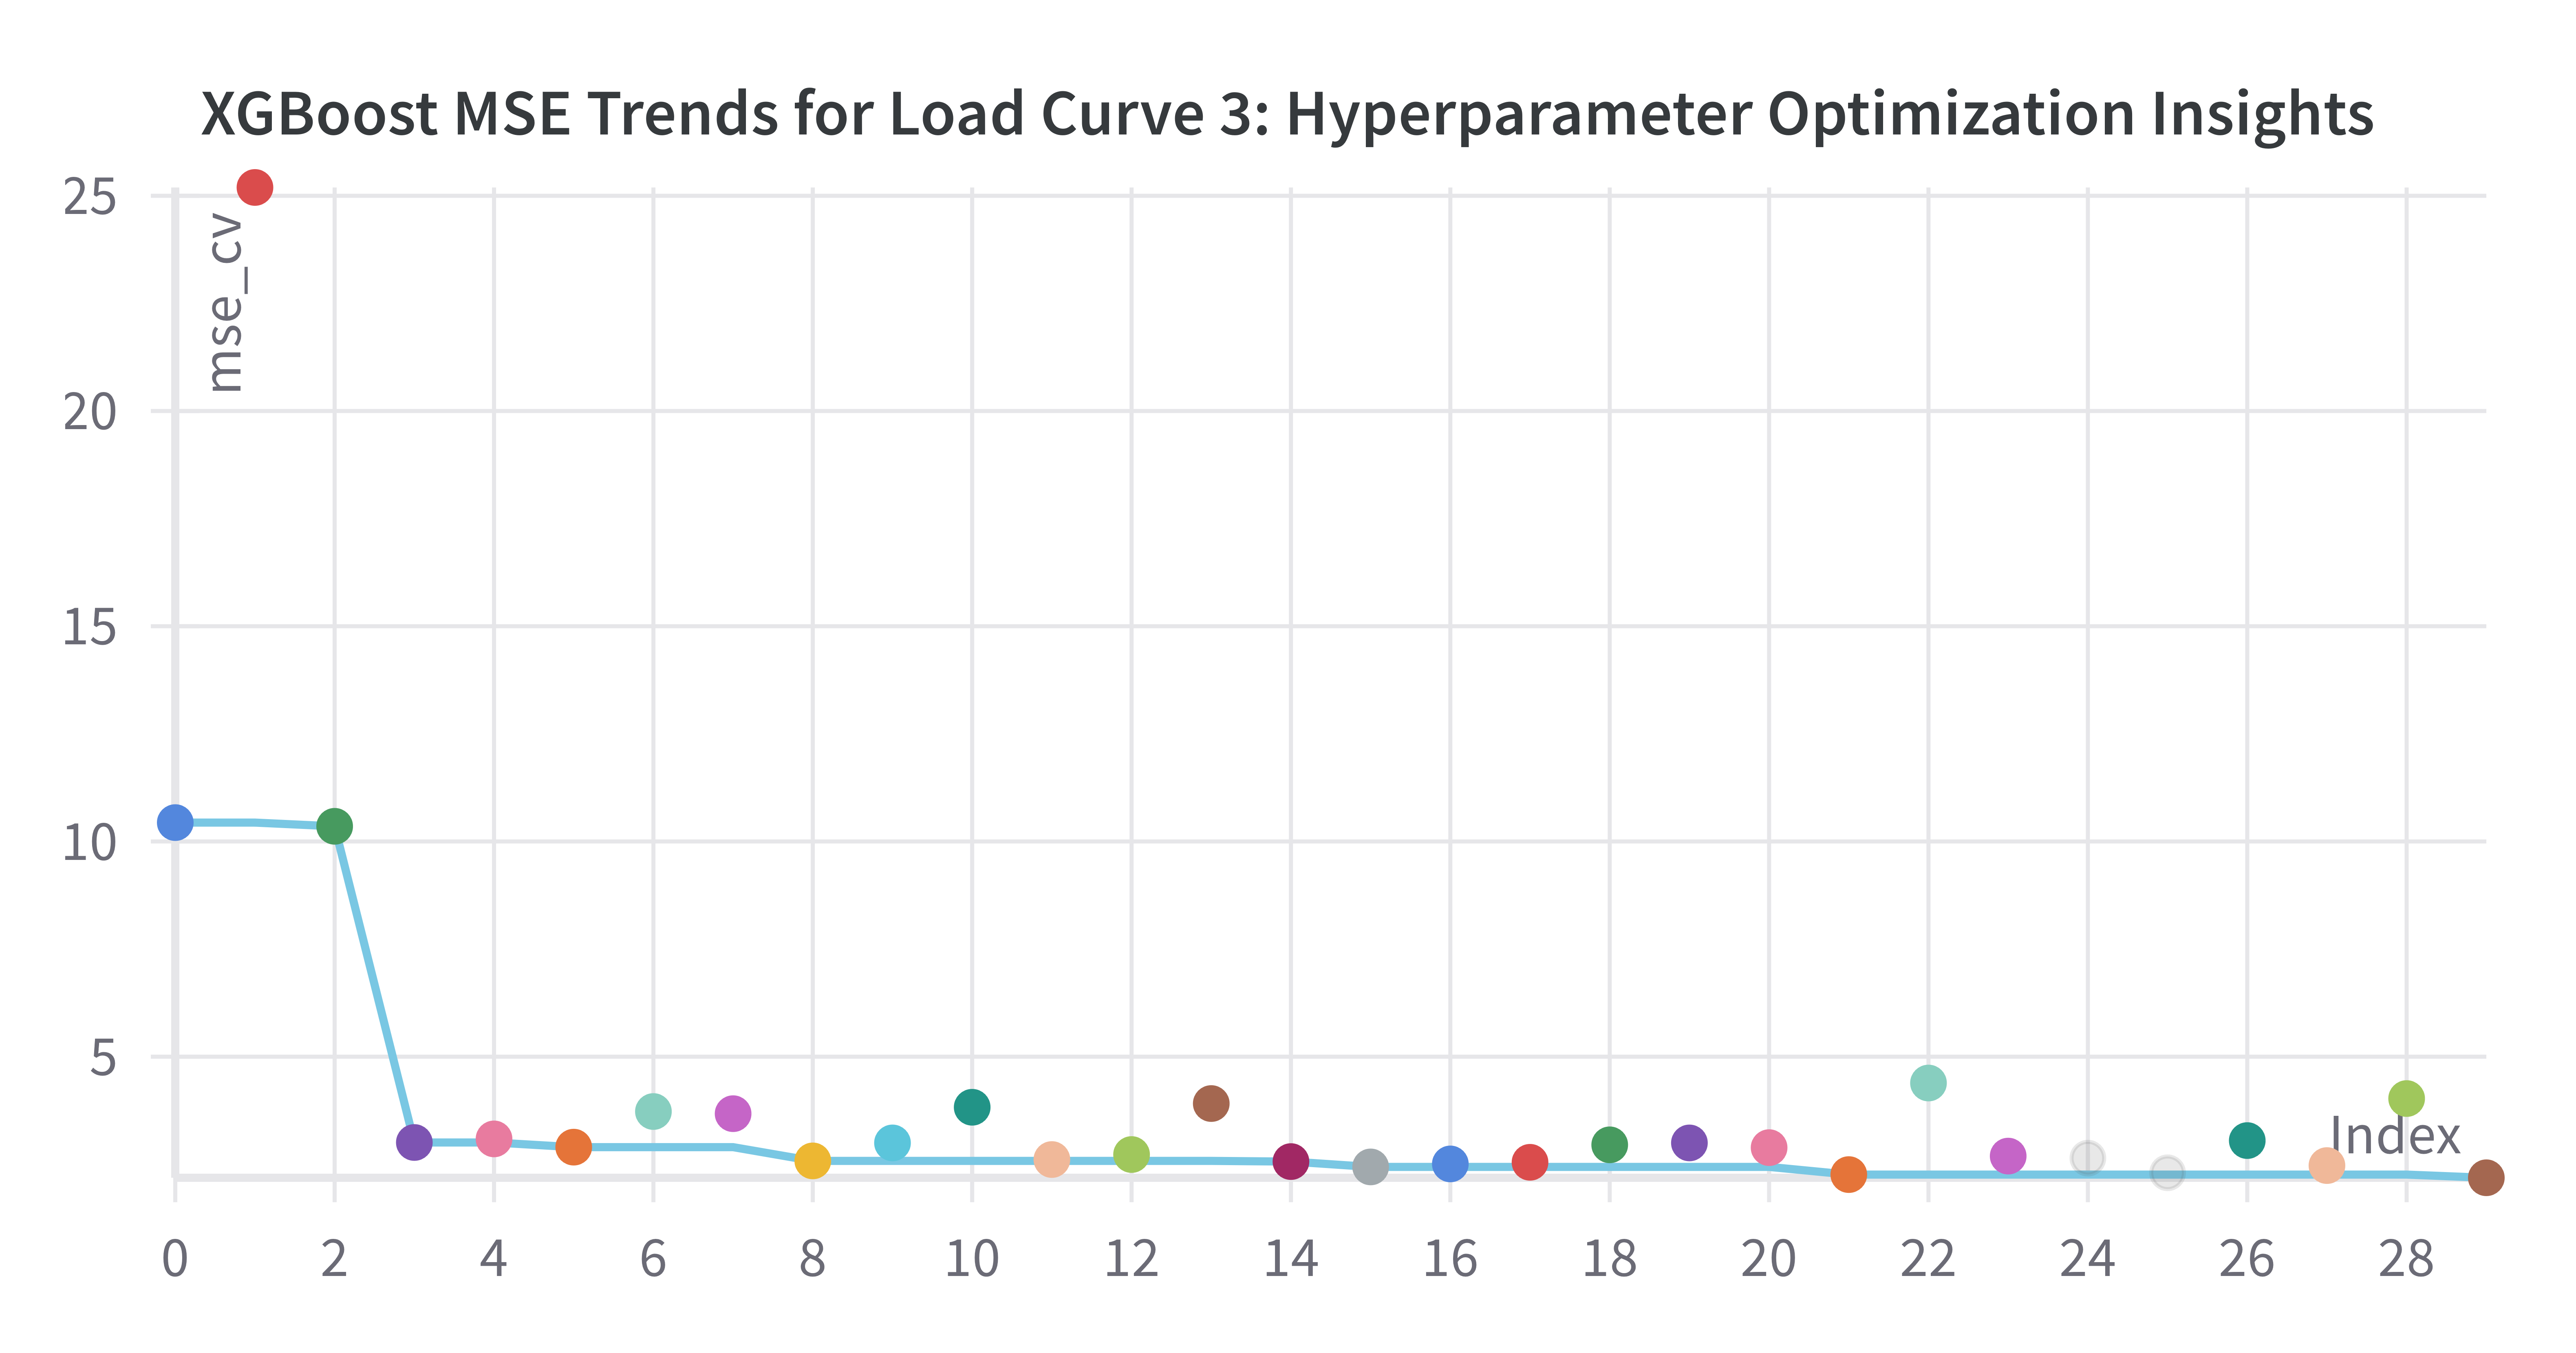
\includegraphics[width=0.75\textwidth]{ressources/Hyperparams/XGBoost/XGBoost MSE Trends for Load Curve 3 Hyperparameter Optimization Insights.png }
    \caption{Bayesian hyperparameter optimization trends for XGBoost on Load Curve 3.}
    \label{fig:xgboost_lc3}
\end{figure}
\subsubsection{Feature importance}
XGBoost's feature importance plots for three different load curves provide insight into the logical parameters that the model considers important for prediction accuracy. The features were ordered according to their importance values.

For Load Curve 1, as illustrated in Figure~\ref{fig:feature_importance_1}, the feature 'holiday' holds the highest significance within the model. Additionally, the feature 'dayofweek' is identified as having great importance in predicting the load curve. Intriguingly, the 'startDate\_minute', 'startDate\_year' and 'startDate\_day' features emerges as the least significant, suggesting that the specific minute, year, and day of the start date bear minimal influence on the target variable. As these are only values that change once a day, there is an opportunity to improve the model by adding external features that change several times a day.
\begin{figure}[H]
    \centering
    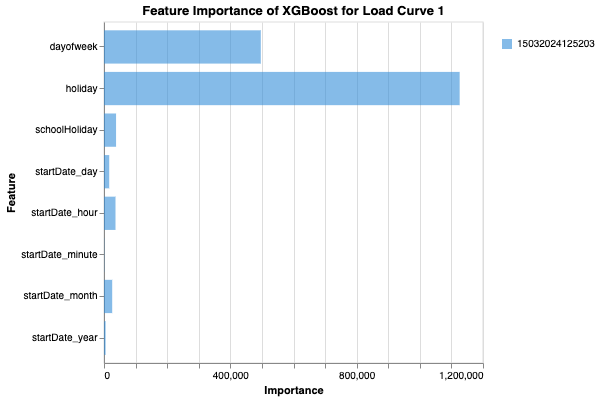
\includegraphics[width=0.75\textwidth]{ressources/FeatureImportance/Feature Importance 1.png}
    \caption{Feature Importance for Load Curve 1.}
    \label{fig:feature_importance_1}
\end{figure}
The graph presented in Figure~\ref{fig:feature_importance_2} demonstrates the feature importance in the XGBoost model for Load Curve 2. Features such as \texttt{avg\_t2\_day} and \texttt{avg\_r2\_month} stand out, suggesting that average temperature and radiation values, calculated over specific time frames, are valuable predictors. These attributes are succeeded by 'startDate\_hour', which likewise hold considerable importance in the model. The feature "holiday" is identified as the least significant, although it was the most important feature for LC1. The ‘t1‘ lag features, representing previous time steps,
show varying degrees of importance, with ‘t1-8‘, ‘t1-6‘ and ‘t1-7‘ being the most influential among them. The number stands for the shift to the previous/future data series. E.g. T1-8 stands for temperature 1 in 2 hour.
\begin{figure}[H]
    \centering
    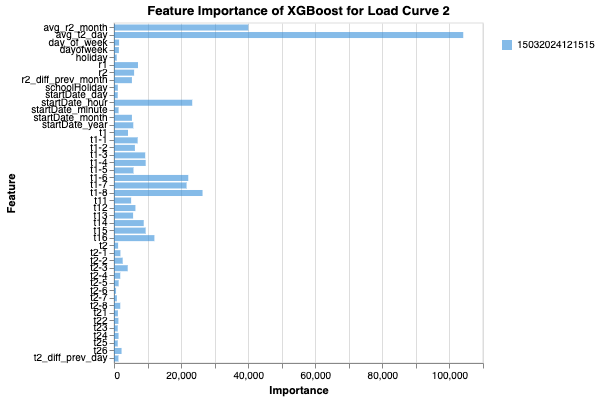
\includegraphics[width=0.75\textwidth]{ressources/FeatureImportance/Feature Importance 2.png}
    \caption{Feature Importance for Load Curve 2.}
    \label{fig:feature_importance_2}
\end{figure}

The analysis of feature importance for Load Curve 3 utilizing XGBoost is presented in Figure \ref{fig:feature_importance_3}. Notably, the features `holiday`, `dayofweek` and `startDate\_hour` exhibit the highest importance scores, suggesting a strong influence on the load curve predictions. These features are followed by `day\_of\_week` and `avg\_t1\_day`, which also play a significant role in the model. Other temporal features such as `avg\_r1\_month` and `schoolHoliday` show moderate importance.The 'r1\_diff\_prev\_month' feature is recognized as having the lowest significance. The `t1` lag features, representing previous time steps, indicate varying degrees of importance, with `t17`, `t15` and `t1-1` being the most influential among them.
\begin{figure}[H]
    \centering
    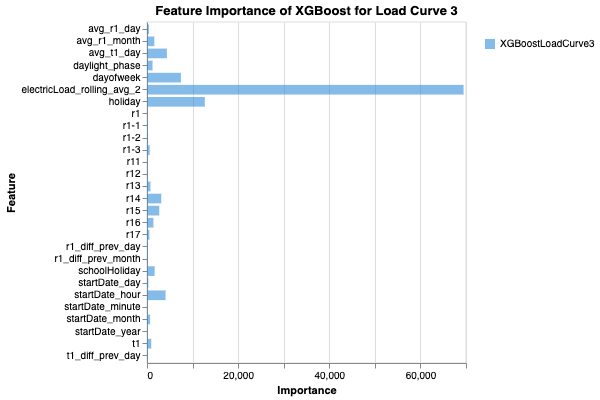
\includegraphics[width=0.75\textwidth]{ressources/FeatureImportance/Feature Importance 3.png}
\caption{Feature importance of XGBoost for Load Curve 3. The importance scores indicate the relative contribution of each feature to the predictive model.}
\label{fig:feature_importance_3}
\end{figure}
Across all three curves, the prominence of features directly related to time and environmental features reaffirms that XGBoost is focusing on logical and interpretable parameters for load forecasting. An expected distribution can be observed. No feature is overly important. This emphasis on temporally relevant features is consistent with domain knowledge in energy demand forecasting, where such factors are known to be influential.

\subsubsection{Final Model Results for XGBoost}
The XGBoost algorithm's efficacy was evaluated across three distinct load curves. The model's performance was quantitatively assessed using \gls*{MSE}, \gls*{MAE}, and the \gls*{R2} metric, which together paint a comprehensive picture of its predictive accuracy and reliability.

The XGBoost model achieved an \gls*{MSE} of 453.107, an \gls*{MAE} of 15.757, and an $R^2$ of 0.959 on Load Curve 1 on the test set. The high \gls*{R2} value indicates that the model explains almost all the variability in the load data. The corresponding residual plot shows a normal distribution of errors centered around zero, signifying precise predictions with no apparent bias. Interestingly, the model performs better on the test data than on the validation data, although it was hyperparameter-optimized with the validation data in the cross-validation procedure. This indicates a good generalization capability.
\begin{figure}[H]
\centering
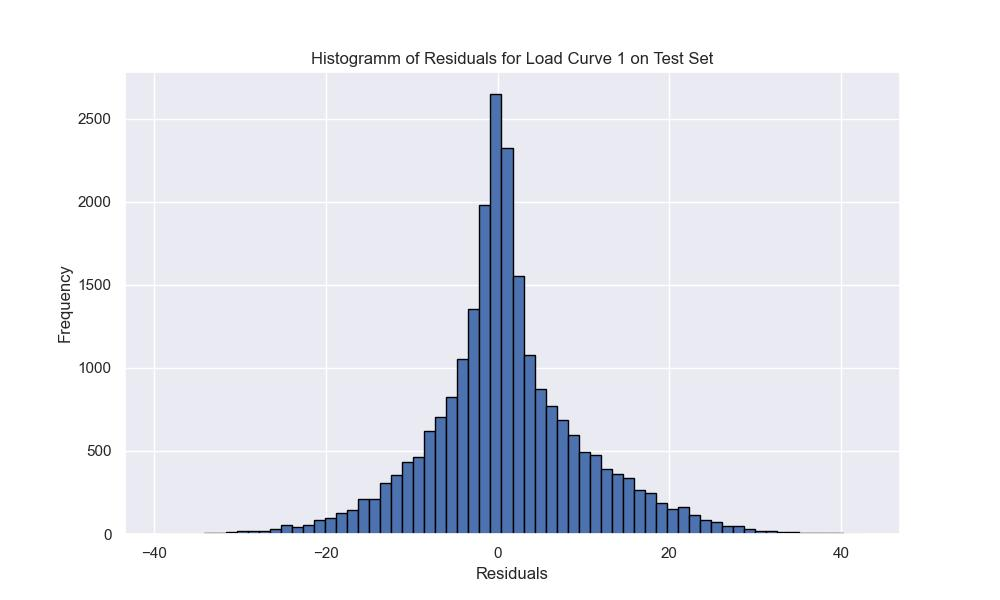
\includegraphics[width=0.8\textwidth]{ressources/residuals/erg/lc1/residuals.jpg}
\caption{Histogram of residuals for Load Curve 1 on the test set, indicating a well-fitted model with symmetrically distributed errors and a a sharp peak around zero.}
\label{fig:residuals_curve1}
\end{figure}

For Load Curve 2, the model delivered an \gls*{MSE} of 11.090, an \gls*{MAE} of 2.600, and an \gls*{R2} of 0.921. The outstandingly low \gls*{MSE} and \gls*{MAE} values suggest that the model's predictions were very close to the actual loads, reflecting high precision and accuracy. The volume of data for Load Curve 2 was the highest, which may have contributed to the model's exceptional performance.
\begin{figure}[H]
\centering
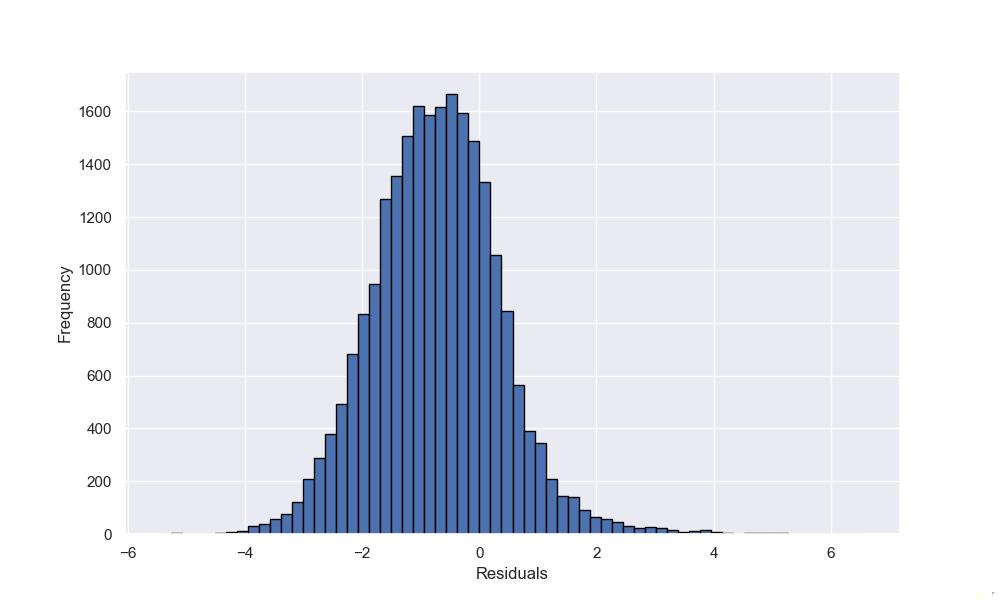
\includegraphics[width=0.8\textwidth]{ressources/residuals/erg/lc2/residuals.jpg}
\caption{Histogram of residuals for Load Curve 2 on the test set, showcasing the model's accuracy with the majority of errors near zero and a slight tendency towards negative residual values.}
\label{fig:residuals_curve2}
\end{figure}

Lastly, on Load Curve 3, the model secured an \gls*{MSE} of 67.493, an \gls*{MAE} of 7.091, and an \gls*{R2} of 0.898. Despite the lower volume of data compared to Load Curve 2, the model still managed to achieve remarkable precision, as evidenced by the high \gls*{R2} value. The residuals' distribution reflects a tight clustering around zero, indicating the model's consistent performance.


\begin{figure}[H]
\centering
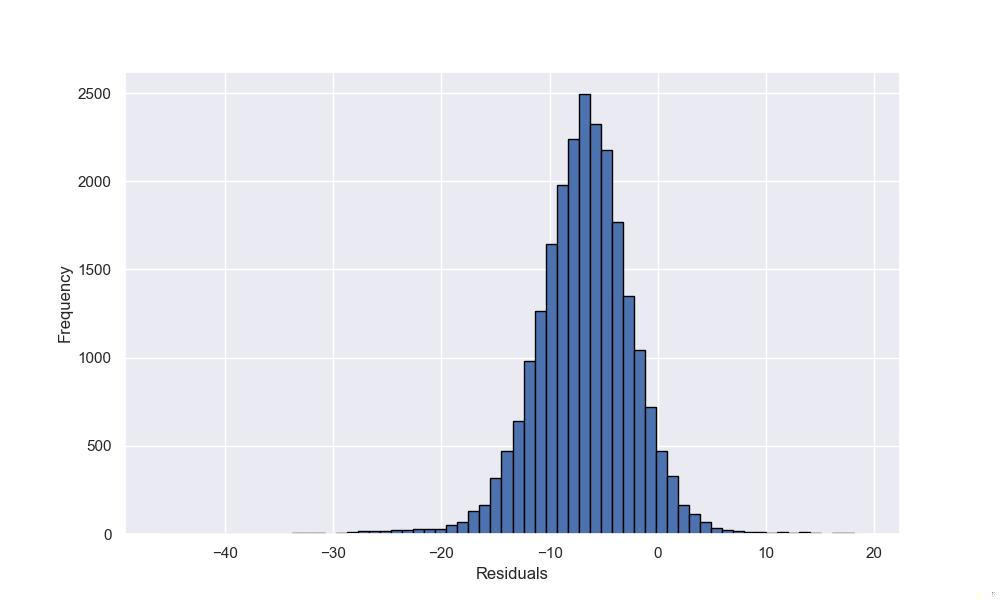
\includegraphics[width=0.8\textwidth]{ressources/residuals/erg/lc3/residuals.jpg}
\caption{Histogram of residuals for Load Curve 3 on the test set, illustrating the model's strong predictive capability with a slight tendency towards negative residual values.}
\label{fig:residuals_curve3}
\end{figure}

To assess the model's performance, an analysis of the residual distributions for each load curve was undertaken. The residuals for Load Curve 1 were found to be symmetrically distributed about zero, which is indicative of an unbiased model, as illustrated in Figure \ref{fig:residuals_curve1}. 
Meanwhile, Load Curve 2 displayed a slight skew towards negative bias, as evident in Figure \ref{fig:residuals_curve2}. Similar observations were made for Load Curve 3, as depicted in Figure \ref{fig:residuals_curve3}. Across all figures, the residuals closely approximate a normal distribution. This observation lends support to the assumption of normally distributed residuals, further validating the robustness of the model's predictive capacity.

\subsection{ARD}
\subsubsection{Analysis of Bayesian Hyperparameter Optimization for ARD}
The analysis of hyperparameter optimization plots for an \gls*{ARD} model across three distinct load curves reveals varied trends and characteristics. The \gls*{MSE} serves as the chosen metric, with each point on the plots representing a model run with a specific set of hyperparameters. 


For Load Curve 1, \gls*{MSE} is almost binary between 5800 and 5500. The two bearings differ by the parameter enable\_daytime\_index. Enabling the value leads to better values. Nevertheless, it can be said that ARD has not found a satisfactory result for Load Curve 1 and this cannot be improved by hyperparameter optimization.
\begin{figure}[H]
    \centering
    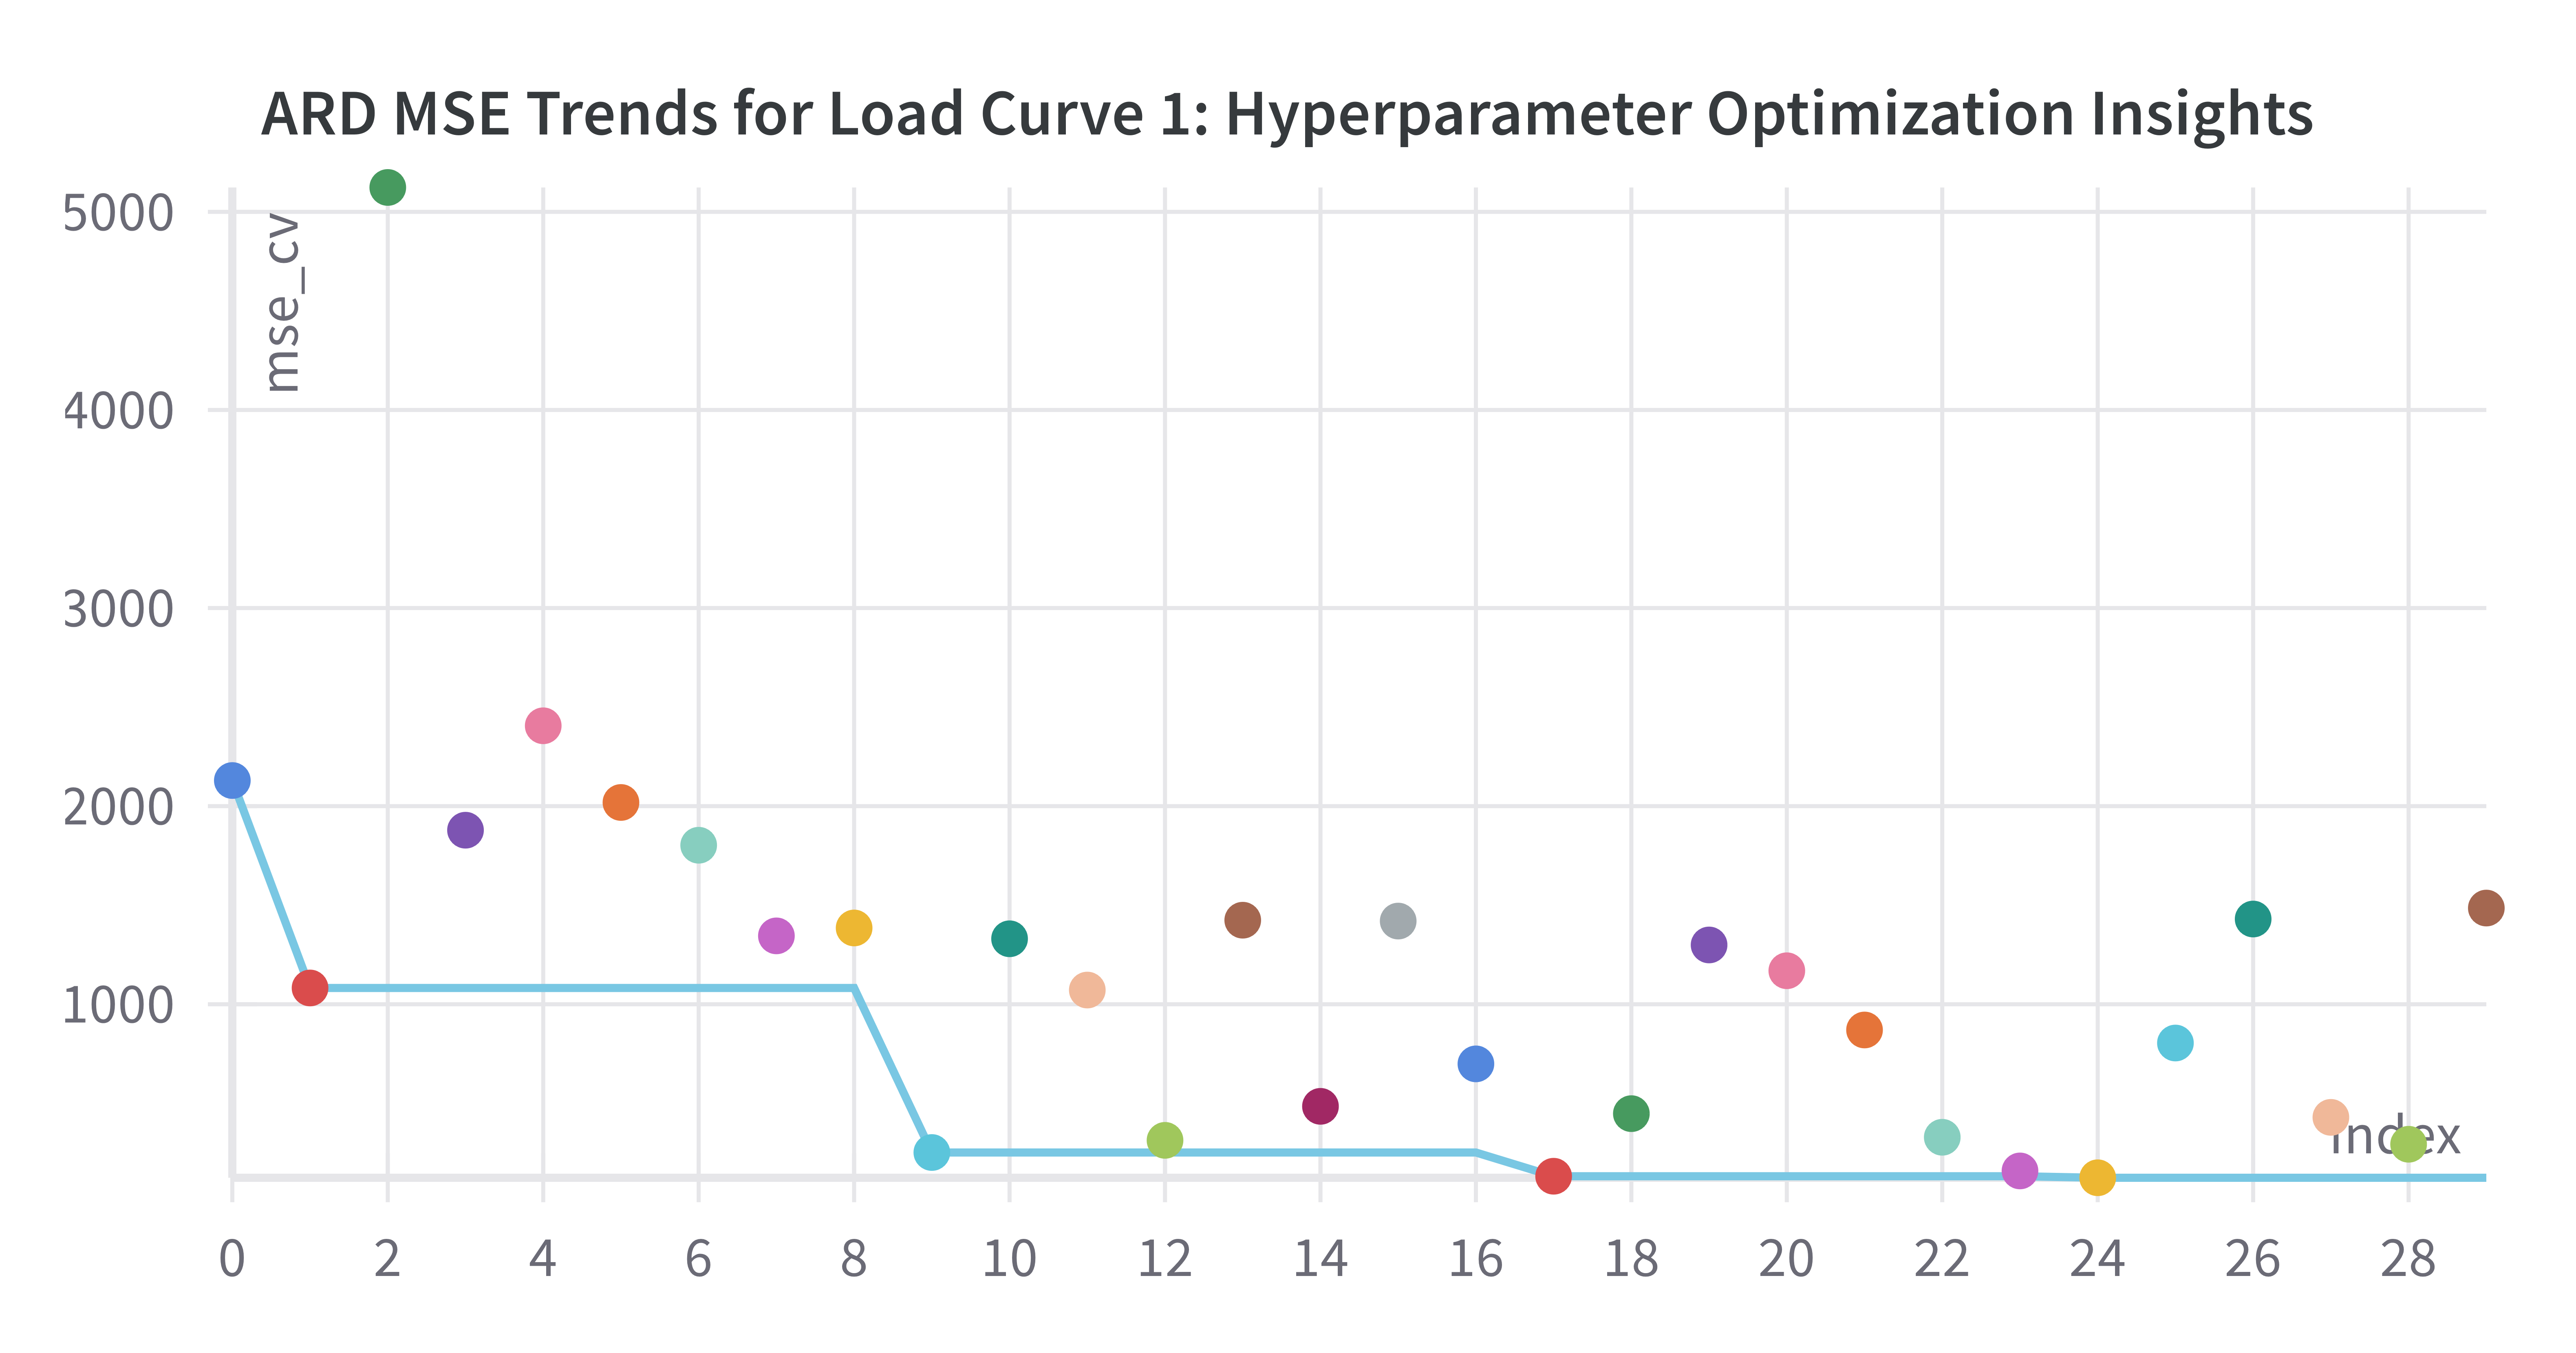
\includegraphics[width=0.75\textwidth]{ressources/Hyperparams/ard/ARD MSE Trends for Load Curve 1 Hyperparameter Optimization Insights.png}
    \caption{Bayesian hyperparameter optimization trends for ARD on Load Curve 1.}
    \label{fig:ard_lc1}
\end{figure}
The optimization narrative for Load Curve 2, depicted in Figure \ref{fig:ard_lc2}, reveals a tight \gls*{MSE} range from about 40 to about 50, implying its more robust to hyperparameter. This robustness is also shown by the fact that no strong change in the MSE was found during optimization.
In the analysis, the \texttt{enable\_daytime\_index} parameter stands out with the highest importance score of 0.3817 and a negative correlation of -0.6178, indicating its significant influence on the model's performance, particularly in diminishing the model's accuracy. The \texttt{shifts} parameter, with an importance score of 0.1384 and a negative correlation of -0.3831, further underscores the impact of temporal shifts on the algorithm's predictions. The \texttt{tol} parameter shows a notable importance score of 0.0867, although its negative correlation of -0.0512 suggests a nuanced effect on model convergence. Other parameters such as \texttt{lambda\_2}, \texttt{compute\_score}, and \texttt{neg\_shifts} exhibit importance scores of 0.0455, 0.0461, and 0.0728, respectively, with their negative correlations indicating varying degrees of influence on the model's prediction accuracy. Interestingly, \texttt{alpha\_1} and \texttt{alpha\_2} present importance scores of 0.071 and 0.0345, with positive correlations of 0.2603 and 0.3726, respectively, suggesting that adjustments in these regularization parameters could potentially enhance the model's performance. The \texttt{load\_lag} and \texttt{n\_iter} parameters, with importance scores of 0.0569 and 0.0537, respectively, show less significant but still noteworthy effects on the model's behavior. The minimal importance score of 0.0129 for \texttt{lambda\_1} and its positive correlation of 0.1368 highlight a lesser but present impact on the model's predictive capability.

\begin{figure}[H]
    \centering
    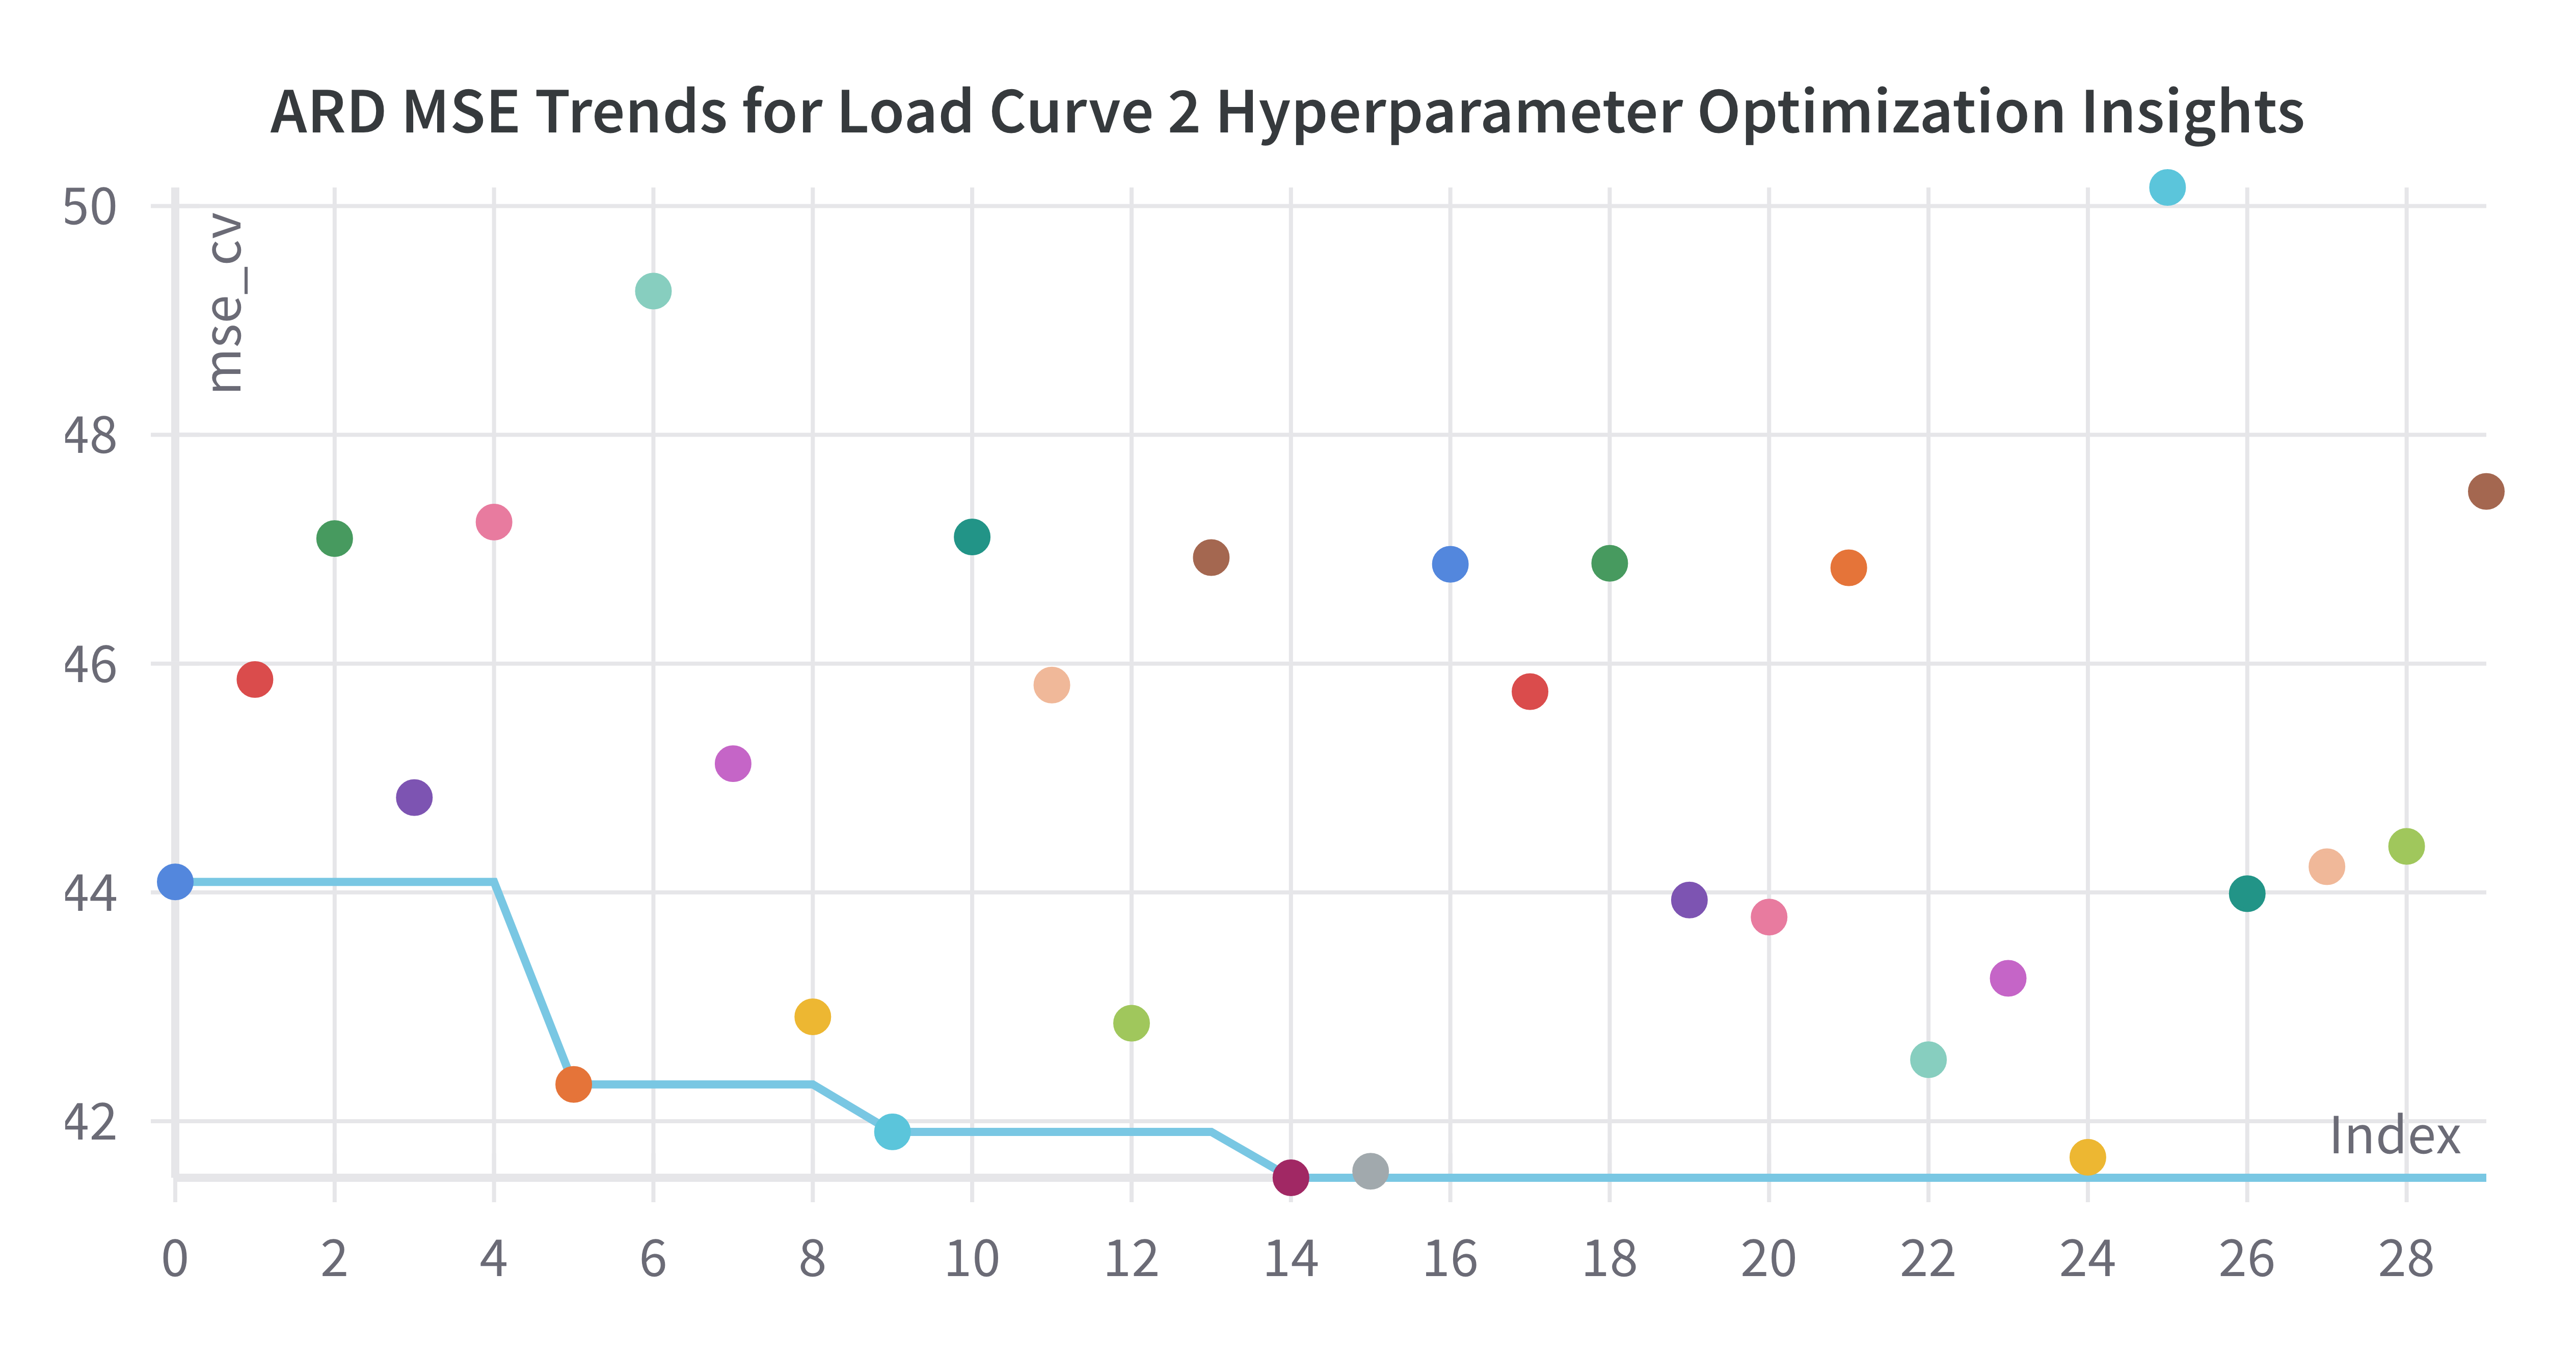
\includegraphics[width=0.75\textwidth]{ressources/Hyperparams/ard/ARD MSE Trends for Load Curve 2 Hyperparameter Optimization Insights.png}
    \caption{Bayesian hyperparameter optimization trends for ARD on Load Curve 2.}
    \label{fig:ard_lc2}
\end{figure}
For Load Curve 3, Figure \ref{fig:ard_lc3} shows a tighter \gls*{MSE} variance across runs, especially at the end of the optimisation. The MSE of the cross validation is usually between 245 and 260, with the smallest MSE being 240.319.
The analysis identifies the \texttt{neg\_shifts} parameter as crucial, with the highest importance score of 0.4063 and a strong positive correlation of 0.6476, underscoring its pivotal role in enhancing the model's accuracy. Similarly, the \texttt{load\_lag} parameter, showing a notable importance score of 0.1498, albeit with a lower correlation of 0.096, suggests its significance in capturing temporal dynamics. The \texttt{shifts} parameter, with an importance score of 0.1241 and a negative correlation of -0.5453, emphasizes the impact of incorporating past temporal information. The \texttt{enable\_daytime\_index}, sharing similarities with the prior analysis, demonstrates considerable importance with a score of 0.0882 and a negative correlation of -0.4398, reinforcing its influence on model performance. \texttt{n\_iter}, with an importance score of 0.1019 and a positive correlation of 0.1845, highlights the model's sensitivity to the number of iterations for convergence. Notably, \texttt{tol}, \texttt{lambda\_2}, and \texttt{compute\_score} parameters exhibit importance scores of 0.0336, 0.0324, and 0.023, with correlations hinting at their nuanced contributions to the model's predictive capabilities. The \texttt{alpha\_1} parameter, although less prominent with an importance score of 0.0132, shows a positive correlation of 0.1608, indicating a role in regularization. In contrast, \texttt{alpha\_2} and \texttt{lambda\_1}, with importance scores of 0.0212 and 0.0064, suggest marginal impacts on model accuracy. 

This analysis, paralleled with observations from LC2, confirms the critical influence of temporal adjustments (\texttt{neg\_shifts}, \texttt{shifts}), regularization parameters (\texttt{alpha\_1}, \texttt{alpha\_2}), and the model's adaptability to the dataset's temporal structure (\texttt{enable\_daytime\_index}) in predicting load curves with precision.

\begin{figure}[H]
    \centering
    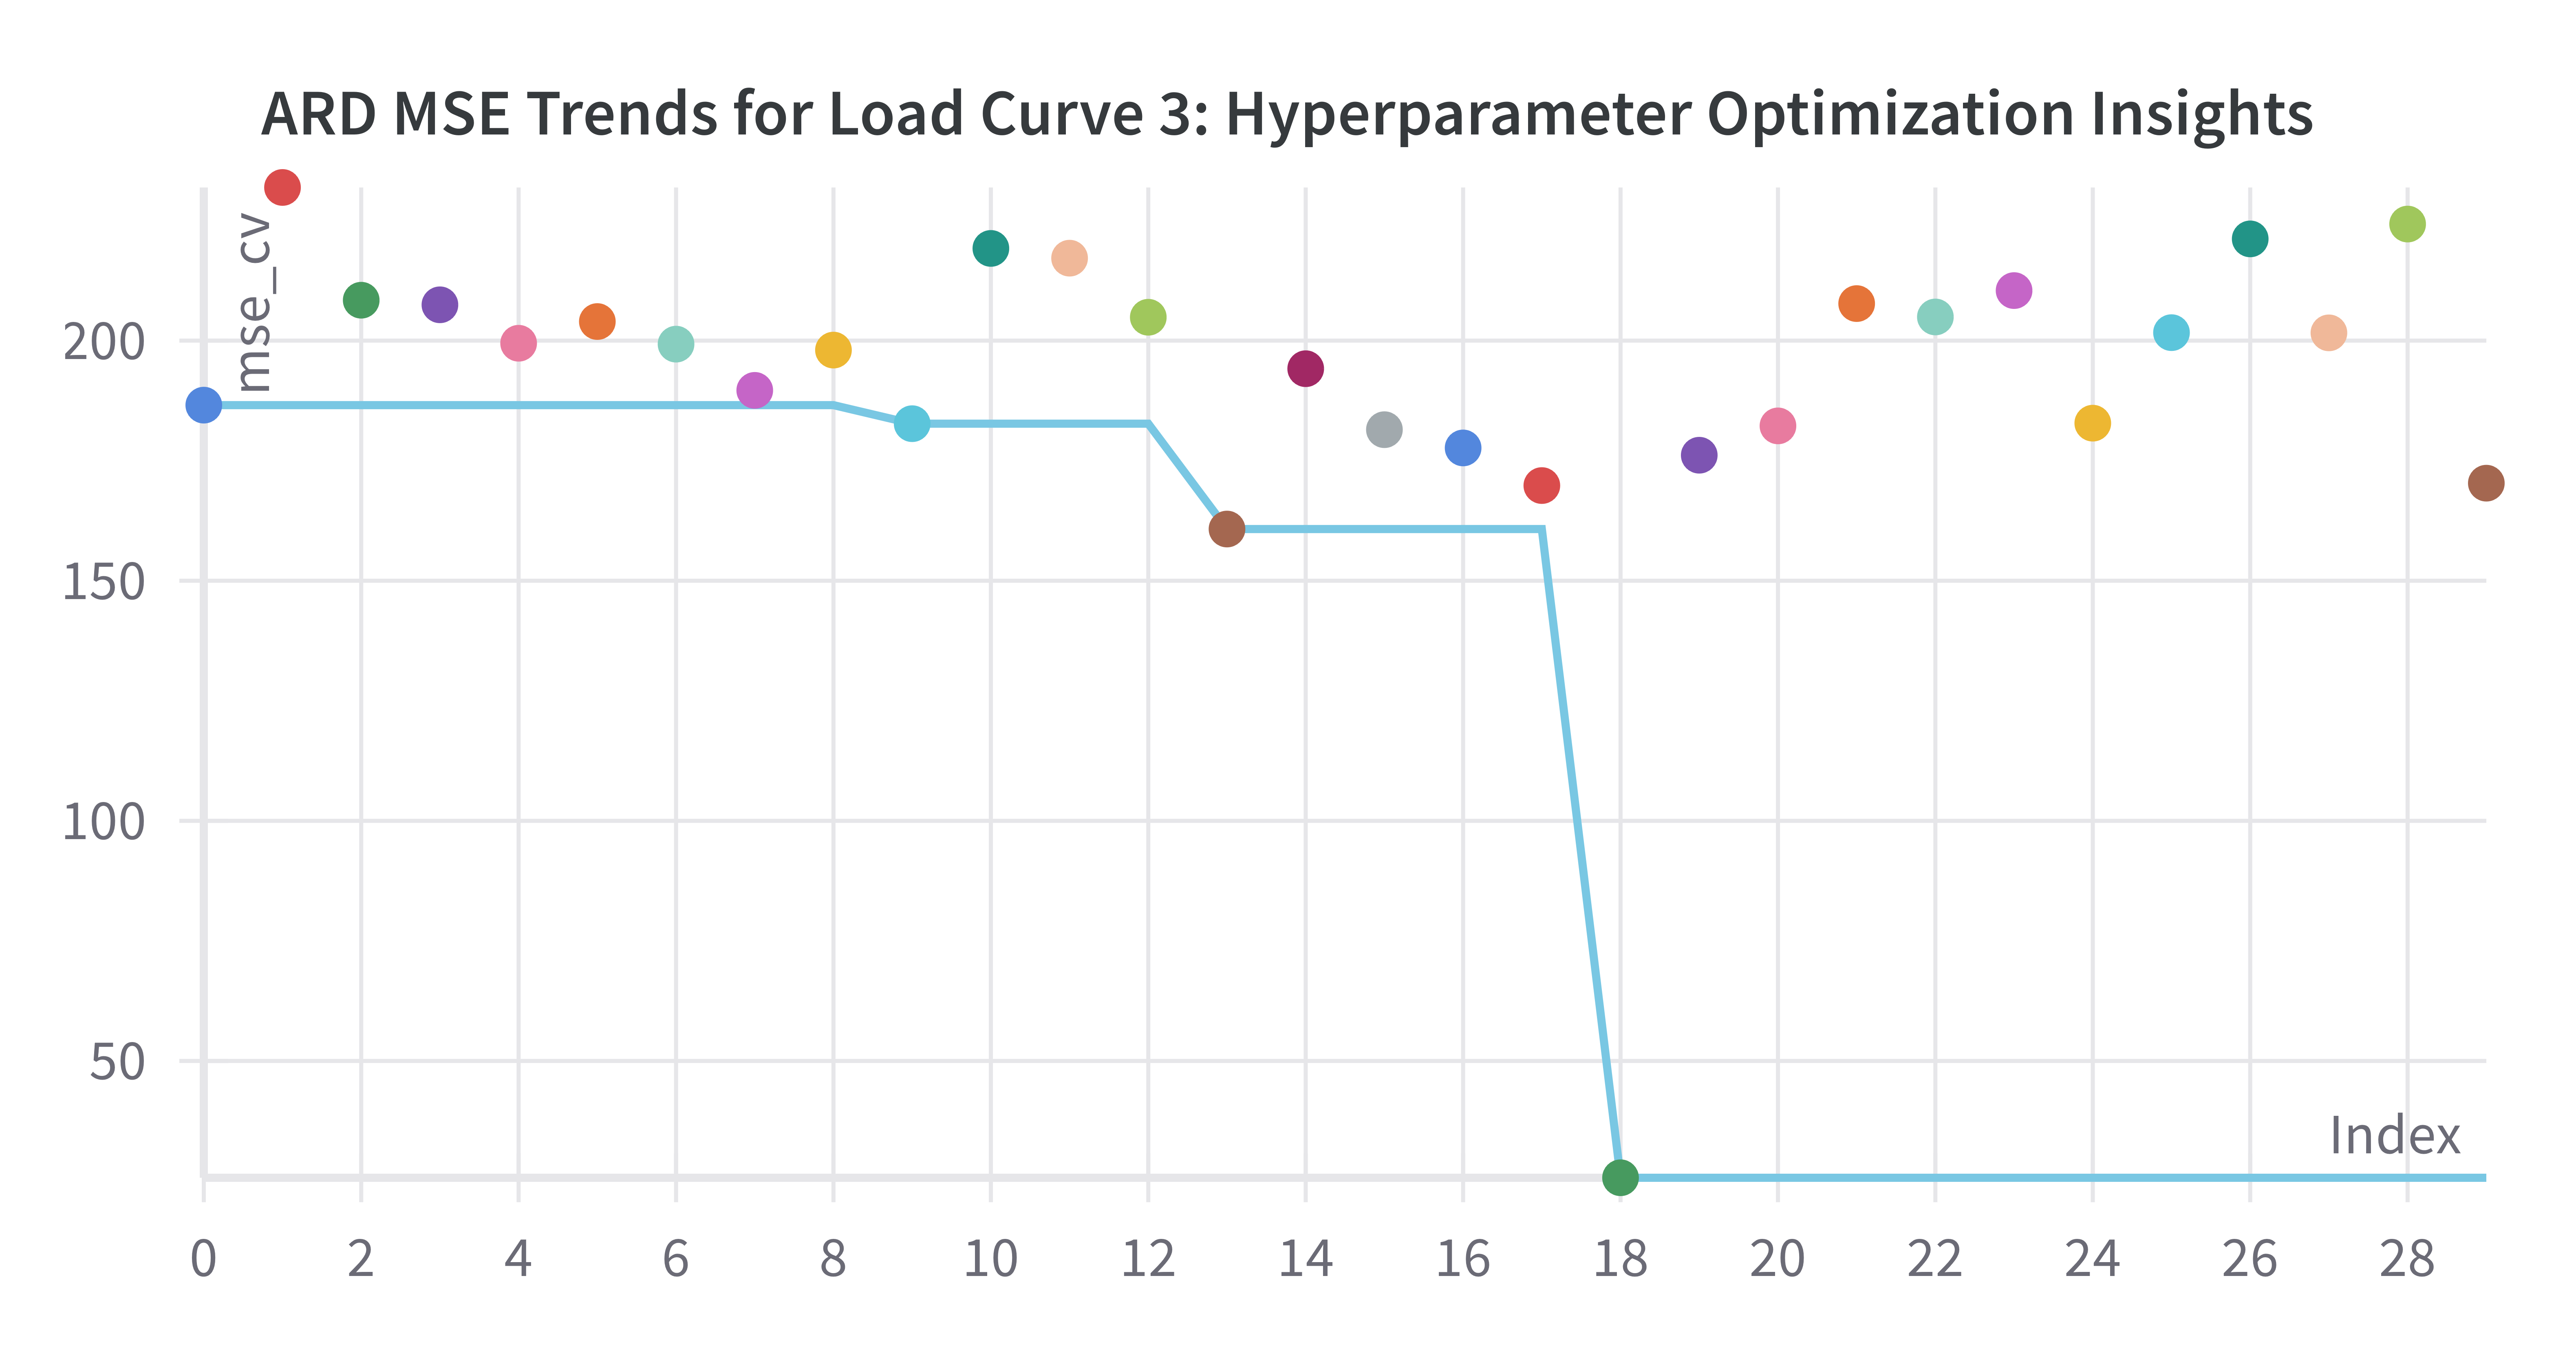
\includegraphics[width=0.75\textwidth]{ressources/Hyperparams/ard/ARD MSE Trends for Load Curve 3 Hyperparameter Optimization Insights.png}
    \caption{Bayesian hyperparameter optimization trends for ARD on Load Curve 3.}
    \label{fig:ard_lc3}
\end{figure}


These tailored hyperparameter settings across different load curves demonstrate the necessity of specific optimization strategies for each forecasting task, ensuring the \gls*{ARD} model's generalizability and resistance to overfitting while maximizing predictive accuracy.

\subsubsection{Final Model Results for ARD}

The \acrshort{ARD} regression model's performance on the test datasets revealed an \acrshort{R2} of 0.44 for \acrshort{LC1}, indicating that the model explains most of the variance. The \acrshort{MAE} and \acrshort{MSE} were at very high values of 63.358 and 6184.419 respectively. This indicates that the model was not able to learn the patterns in the data. For \acrshort{LC2}, the model achieved an \acrshort{R2} of 0.757, with a corresponding \acrshort{MAE} of 4.644 and \acrshort{MSE} of 34.239 , reflecting a decent fit of the model to the data, much better than for \acrshort{LC1}. \acrshort{LC3} recorded an \acrshort{R2} of 0.618, with \acrshort{MAE} and \acrshort{MSE} values of 12.792 and 253.466, respectively, which indicates that ARD has learned the pattern in the data but is still not fit perfectly. In general, the model reproduces the underlying patterns for LC2 and LC3 but is still characterized by high errors. 


\subsection{KNN}
\subsubsection{Analysis of Bayesian Hyperparameter Optimization for KNN}

As visualized in Figure \ref{fig:knn_lc1} for LC1, the variance of the MSE values could be optimized in the course of training, which means that the hyperparameter optimization was successful. At the beginning of the optimization process, the MSE values had a large spread. It can be seen that the trend of the MSE values is decreasing and reaches a minimum of 3115.41.
Particularly important in the hyperparameter optimization was the number of neighbors with a correlation of 0.929 and the p with a correlation of 0.757. Nevertheless, the results of KNN are not good.   
The \texttt{n\_neighbors} parameter, characterized by an importance score of 0.8325 and a positive correlation of 0.9293, emerges as the most influential in determining the model's performance, suggesting the critical role of the neighborhood size in the algorithm's predictions. Additionally, the \texttt{p} value, with an importance score of 0.0841 and a strong positive correlation of 0.7568, highlights the significance of the distance metric used in the k-nearest neighbors algorithm. Other parameters, such as \texttt{shifts} and \texttt{neg\_shifts}, exhibit lesser importance scores of 0.0201 and 0.0143, respectively, but their correlations (-0.487 for \texttt{shifts} and 0.3 for \texttt{neg\_shifts}) suggest their nuanced impact on the model's behavior. The \texttt{leaf\_size}, with an importance score of 0.0293 and a correlation of 0.2454, also plays a role, albeit less critical than \texttt{n\_neighbors} and \texttt{p}. Interestingly, \texttt{enable\_daytime\_index}, despite being considered in the model, show minimal importance scores of 0.0091 and 0.0106, respectively, indicating a marginal effect on the overall model performance.


\begin{figure}[H]
    \centering
    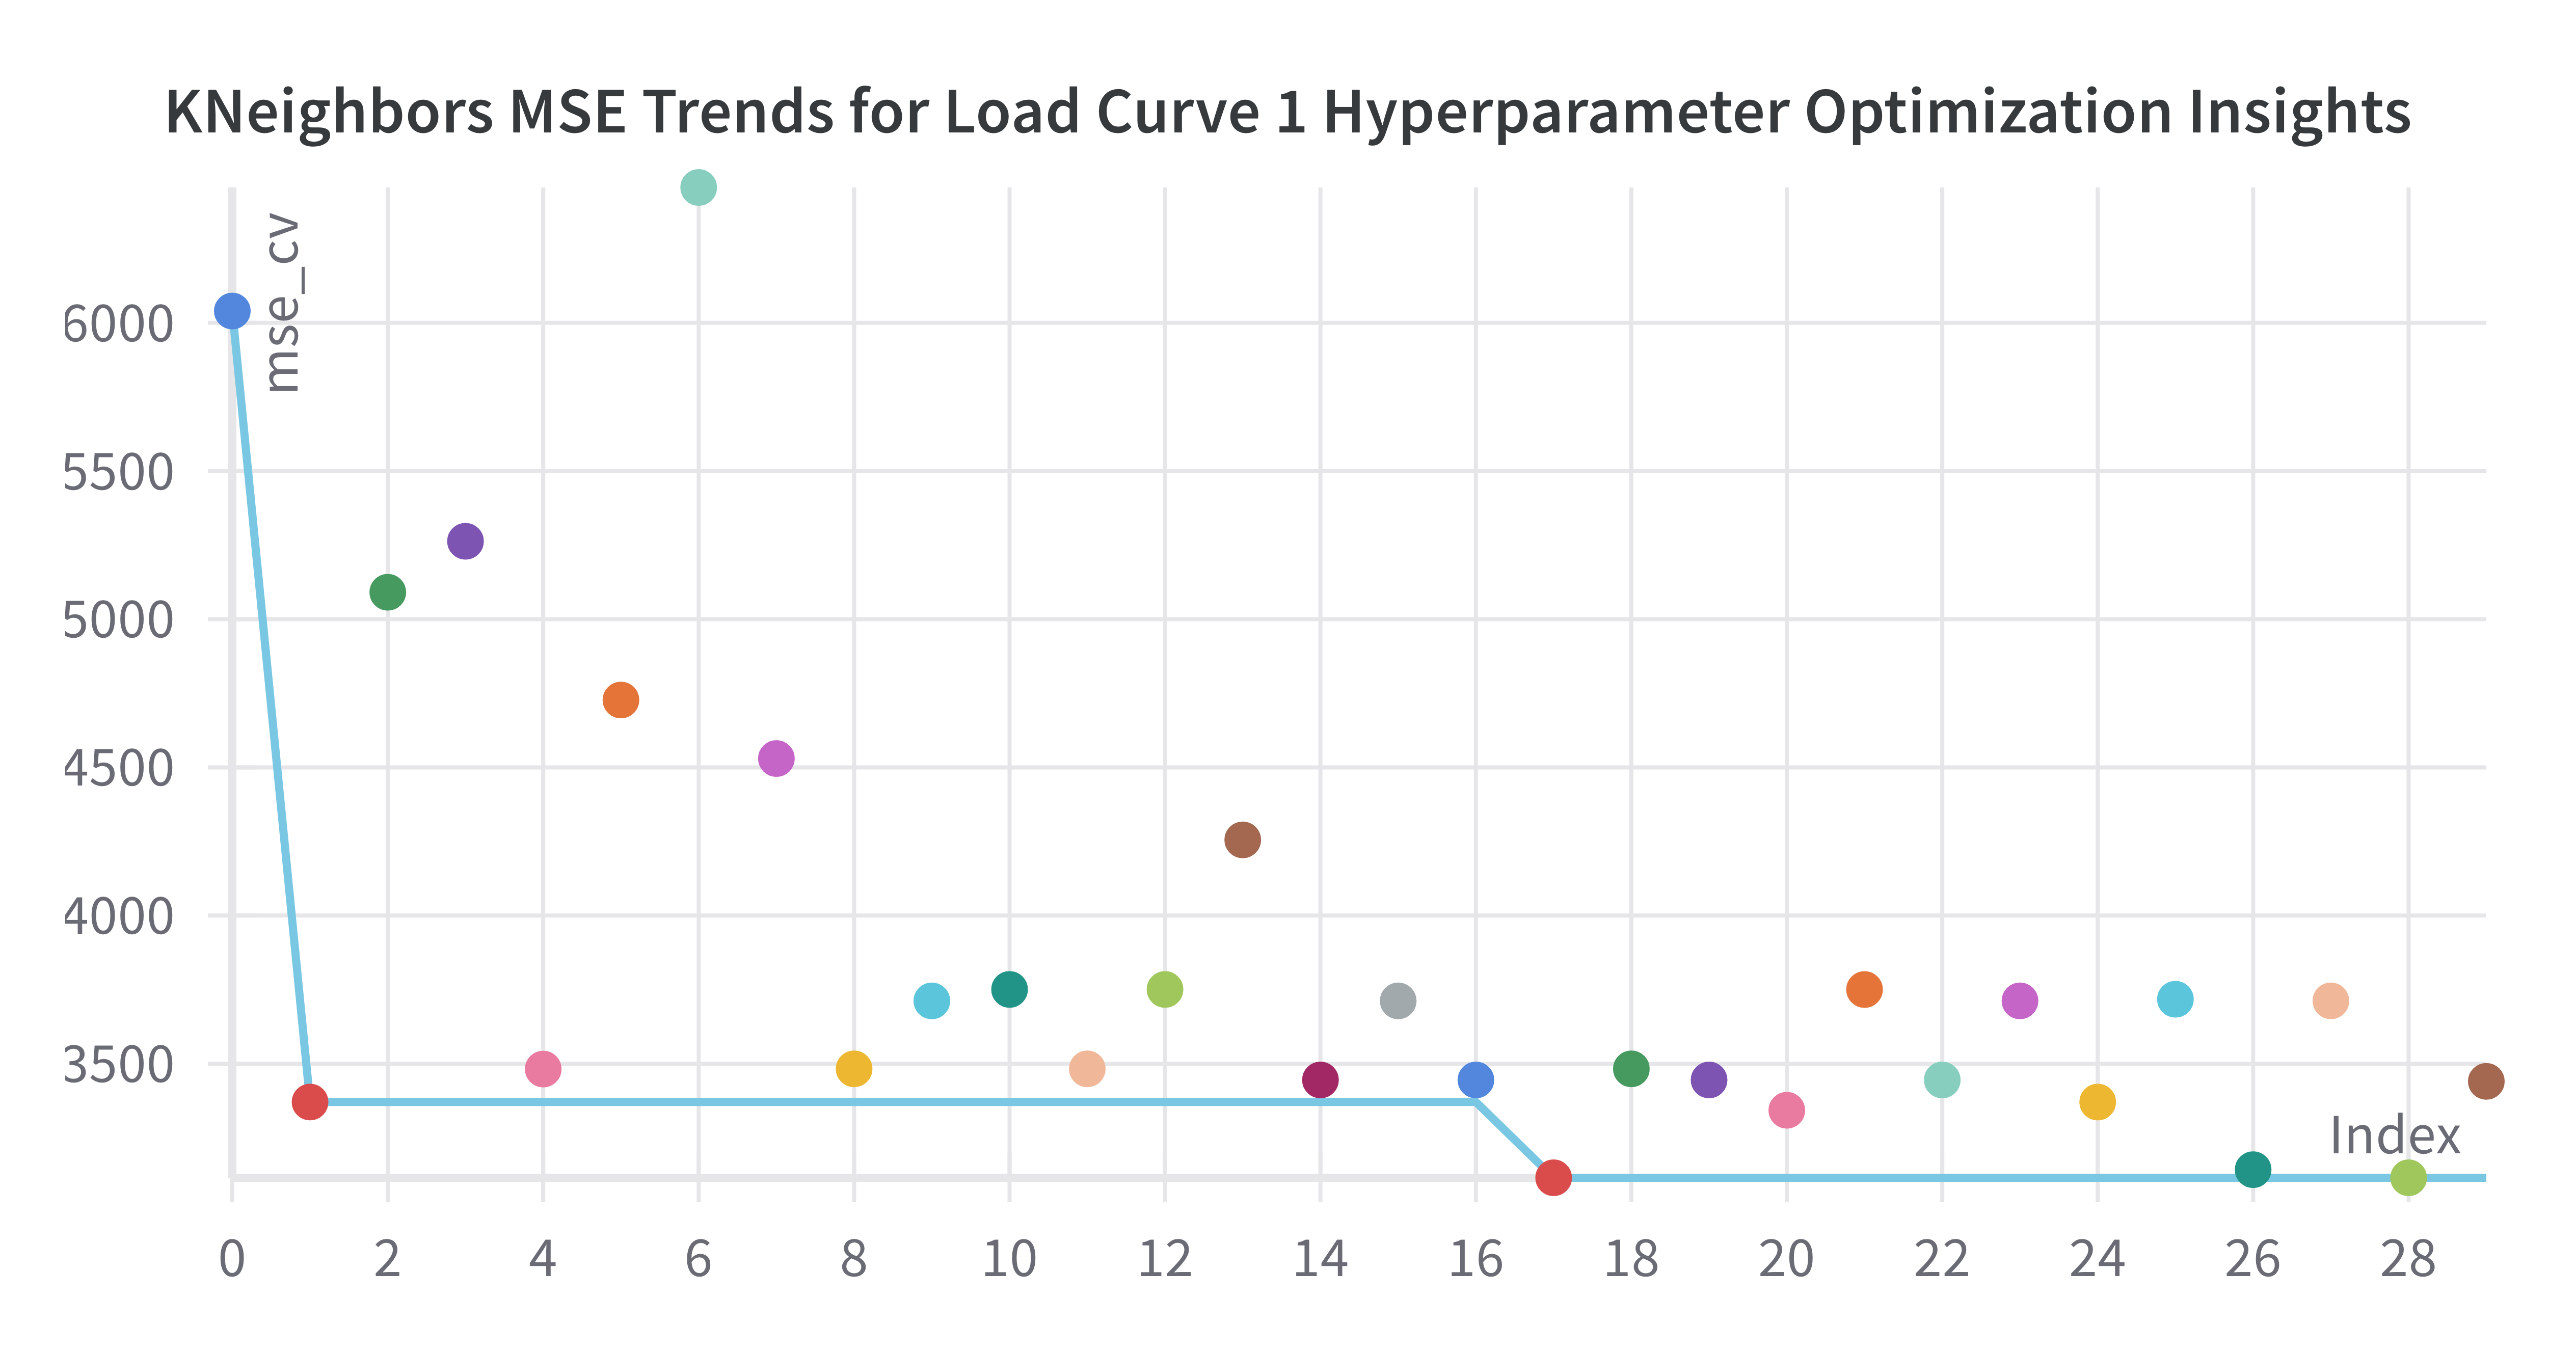
\includegraphics[width=0.75\textwidth]{ressources/Hyperparams/KNN/KNeighbors MSE Trends for Load Curve 1 Hyperparameter Optimization Insights.png}
    \caption{Hyperparameter optimization trends for KNN on Load Curve 1.}
    \label{fig:knn_lc1}
\end{figure}

The Bayesian optimization for the \gls*{KNN} model on load curve 2 shows a steady decrease in the variance of the \gls*{MSE} and is visualized in Figure \ref{fig:knn_lc2}. Coincidentally, in the first run a low MSE of 36.895 was already achieved, but this could be improved again at the end. The lowest MSE is 36.81.

The optimal configuration, which utilizes a `leaf\_size` of 83 and `n\_neighbors` of 100, underscores the model's sensitivity to the neighborhood size and tree complexity. 

Conversely, the `shifts` parameter, with a significant correlation (-0.266), and a value of 7, points to the relevance of incorporating inverse temporal dynamics, potentially capturing the lags in the data. The `p` value of 1 indicates the utilization of Manhattan distance, which might be beneficial for this specific dataset by considering the absolute differences between the time steps.

Interestingly, the `enable\_daytime\_index` was set to true, although it showed a slight negative correlation (-0.032) with the model's performance. This could imply that while the time of day is informative, it may not always contribute positively to the predictive accuracy for this particular load curve. The absence of `enable\_day\_of\_week\_index` in the best configuration, despite its positive correlation (0.364), might suggest its lesser predictive power compared to other features within the dataset.

In summary, the Bayesian hyperparameter optimization reveals a nuanced interplay of temporal features and algorithmic parameters in shaping the \gls*{KNN} model's predictions, leading to a set of hyperparameters that are well-aligned with the underlying patterns of Load Curve 2.

\begin{figure}[H]
    \centering
    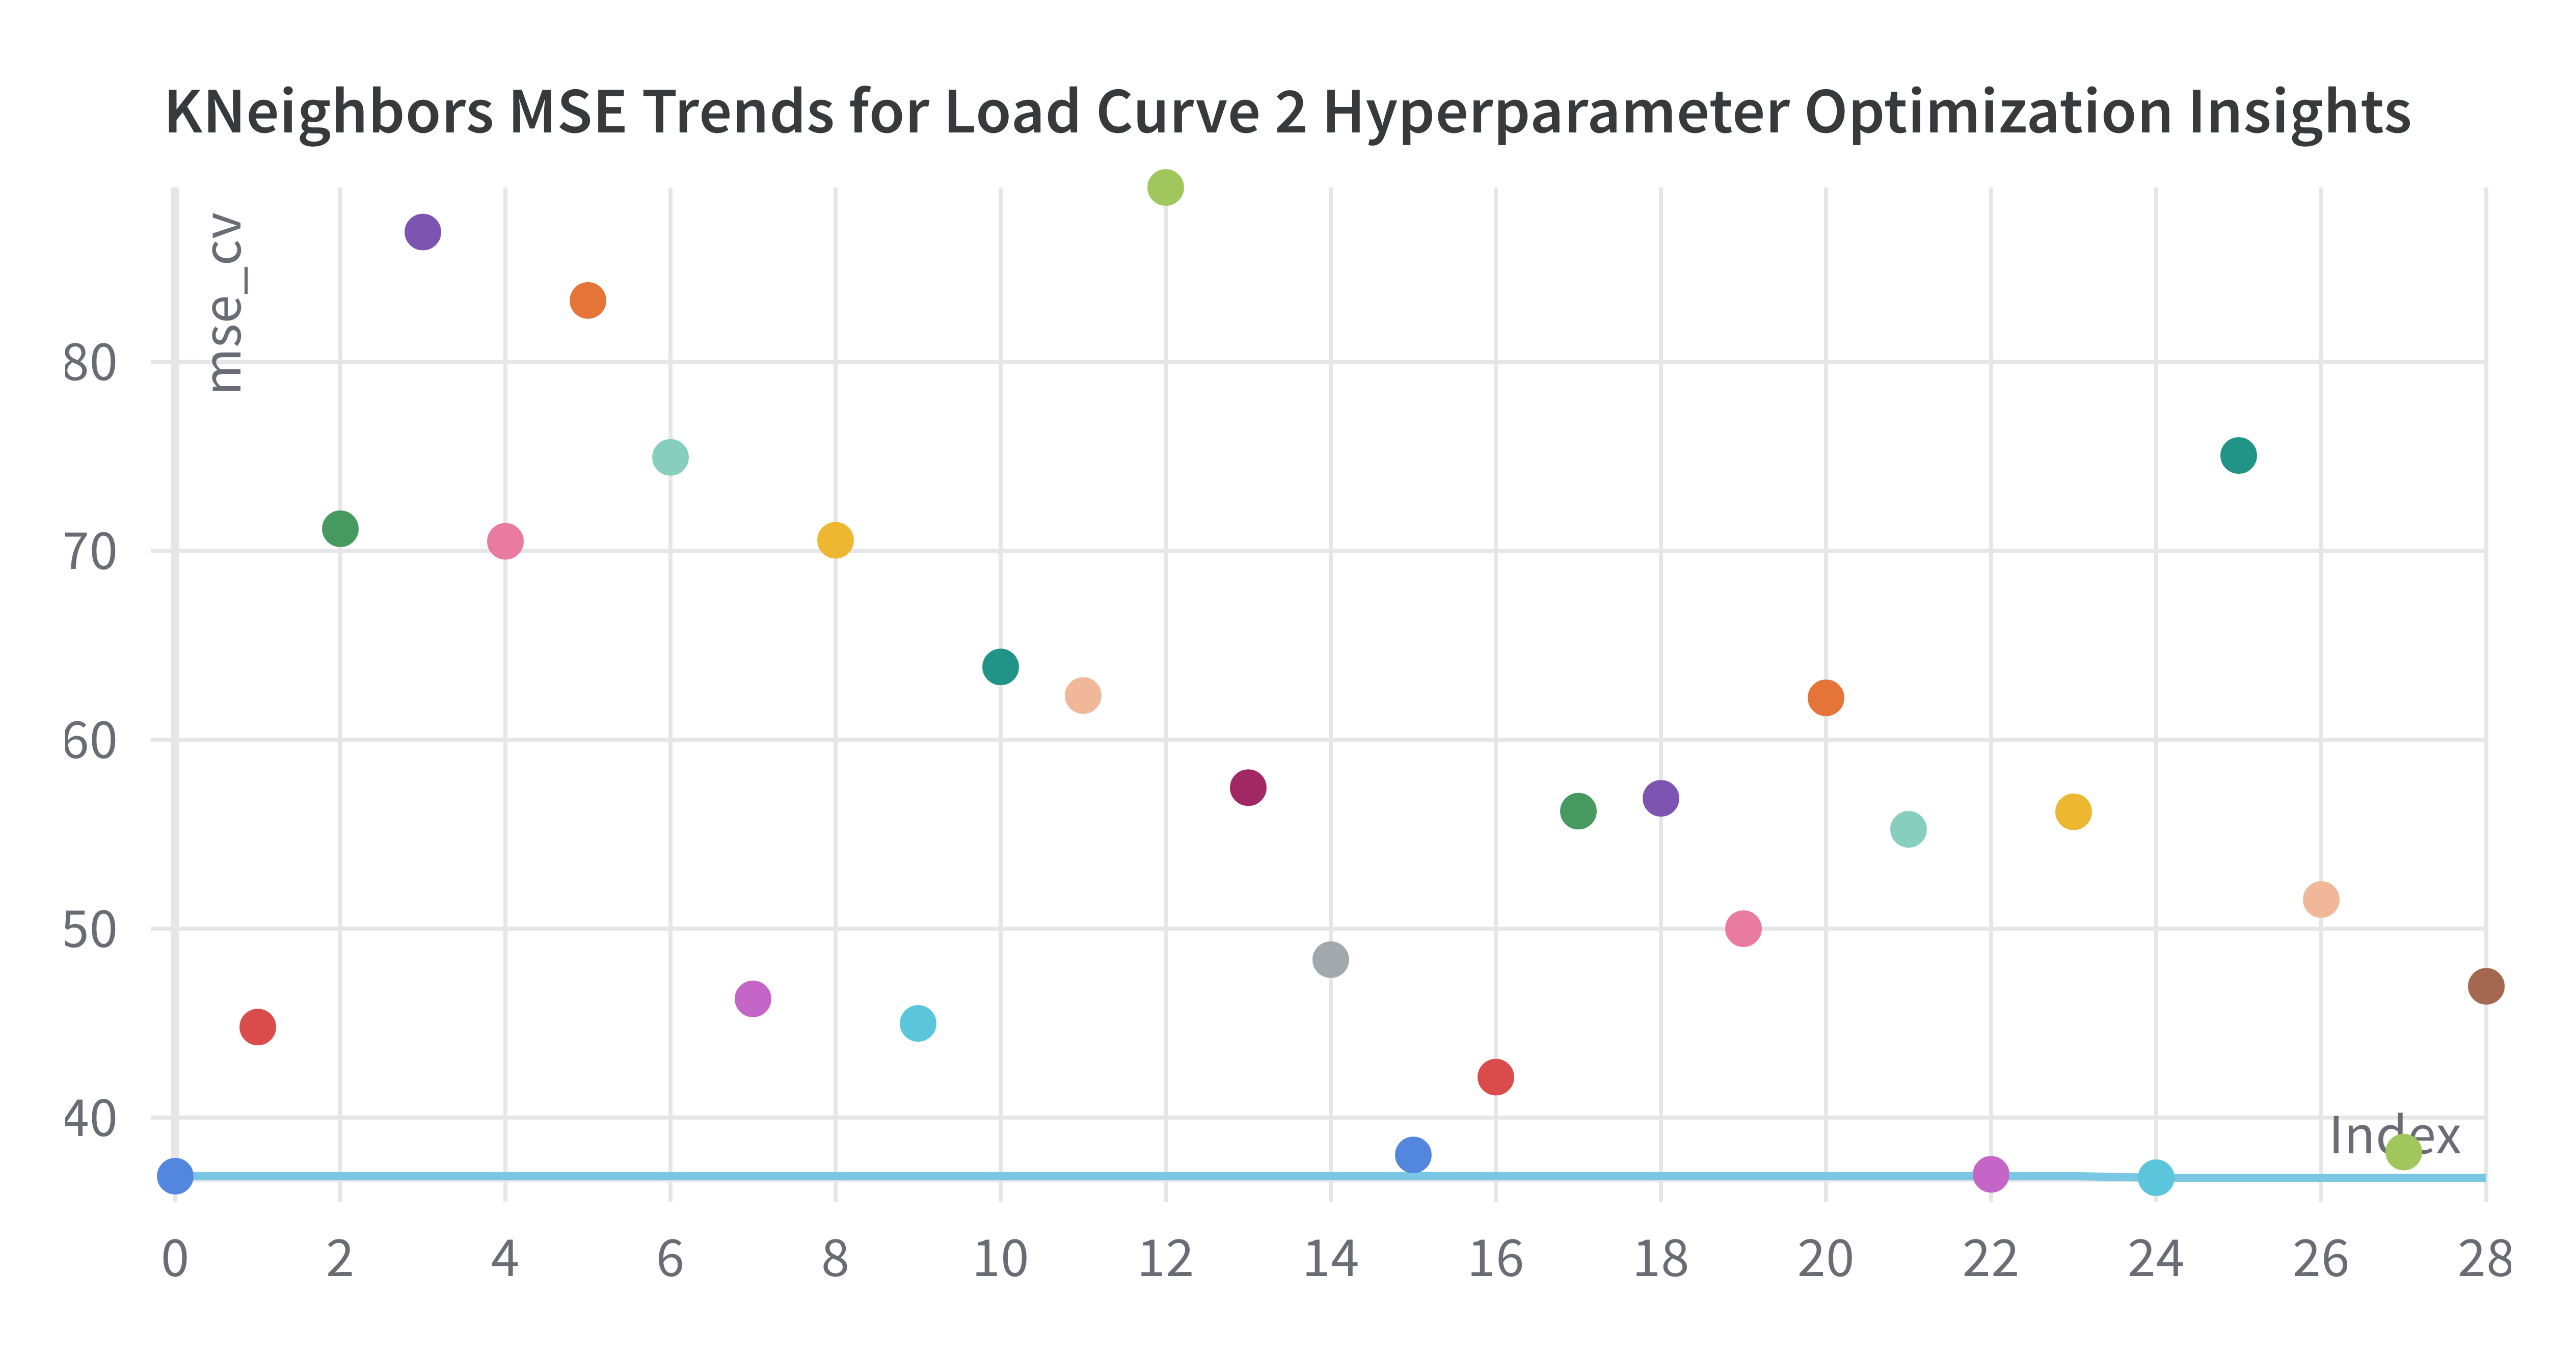
\includegraphics[width=0.75\textwidth]{ressources/Hyperparams/KNN/KNeighbors MSE Trends for Load Curve 2 Hyperparameter Optimization Insights.png}
    \caption{Bayesian hyperparameter optimization trends for KNN on Load Curve 2.}
    \label{fig:knn_lc2}
\end{figure}

In analyzing the Bayesian hyperparameter optimization, visualized in  for \gls*{KNN} concerning Load Curve 3, we observe a small optimization trajectory with a downward trend in \gls*{MSE}, achieving a minimum of 330.876. This result showcases the ability of \gls*{KNN} to adapt to different load scenarios, even within complex datasets. The chosen hyperparameters indicate a preference for `kd\_tree` as the algorithm and a `leaf\_size` of 40, optimizing the balance between computational efficiency and prediction fidelity. 

The parameter `p`, with a value of 1, corresponds to the Manhattan distance and suggests that in this context, the simpler measure of distance outperforms more complex metrics. Interestingly, `n\_neighbors` set at 300 and the absence of negative shifts (`neg\_shifts` of -5) indicate a model that leans on a larger neighborhood for predictions, diverging from the inclination towards smaller neighborhoods in other load curves.

Despite the `enable\_daytime\_index` parameter showing only a modest negativ correlation (-0.187), its inclusion in the optimal configuration implies that time-of-day effects, while subtle, are still considered by the model when forecasting load. This is in contrast to the `enable\_day\_of\_week\_index`, which is not included, suggesting less predictive power from day-of-week effects for Load Curve 3.

The analytical process thus reflects a finely-tuned \gls*{KNN} model that incorporates logical and statistically significant parameters to enhance predictive performance for Load Curve 3.

\begin{figure}[H]
    \centering
    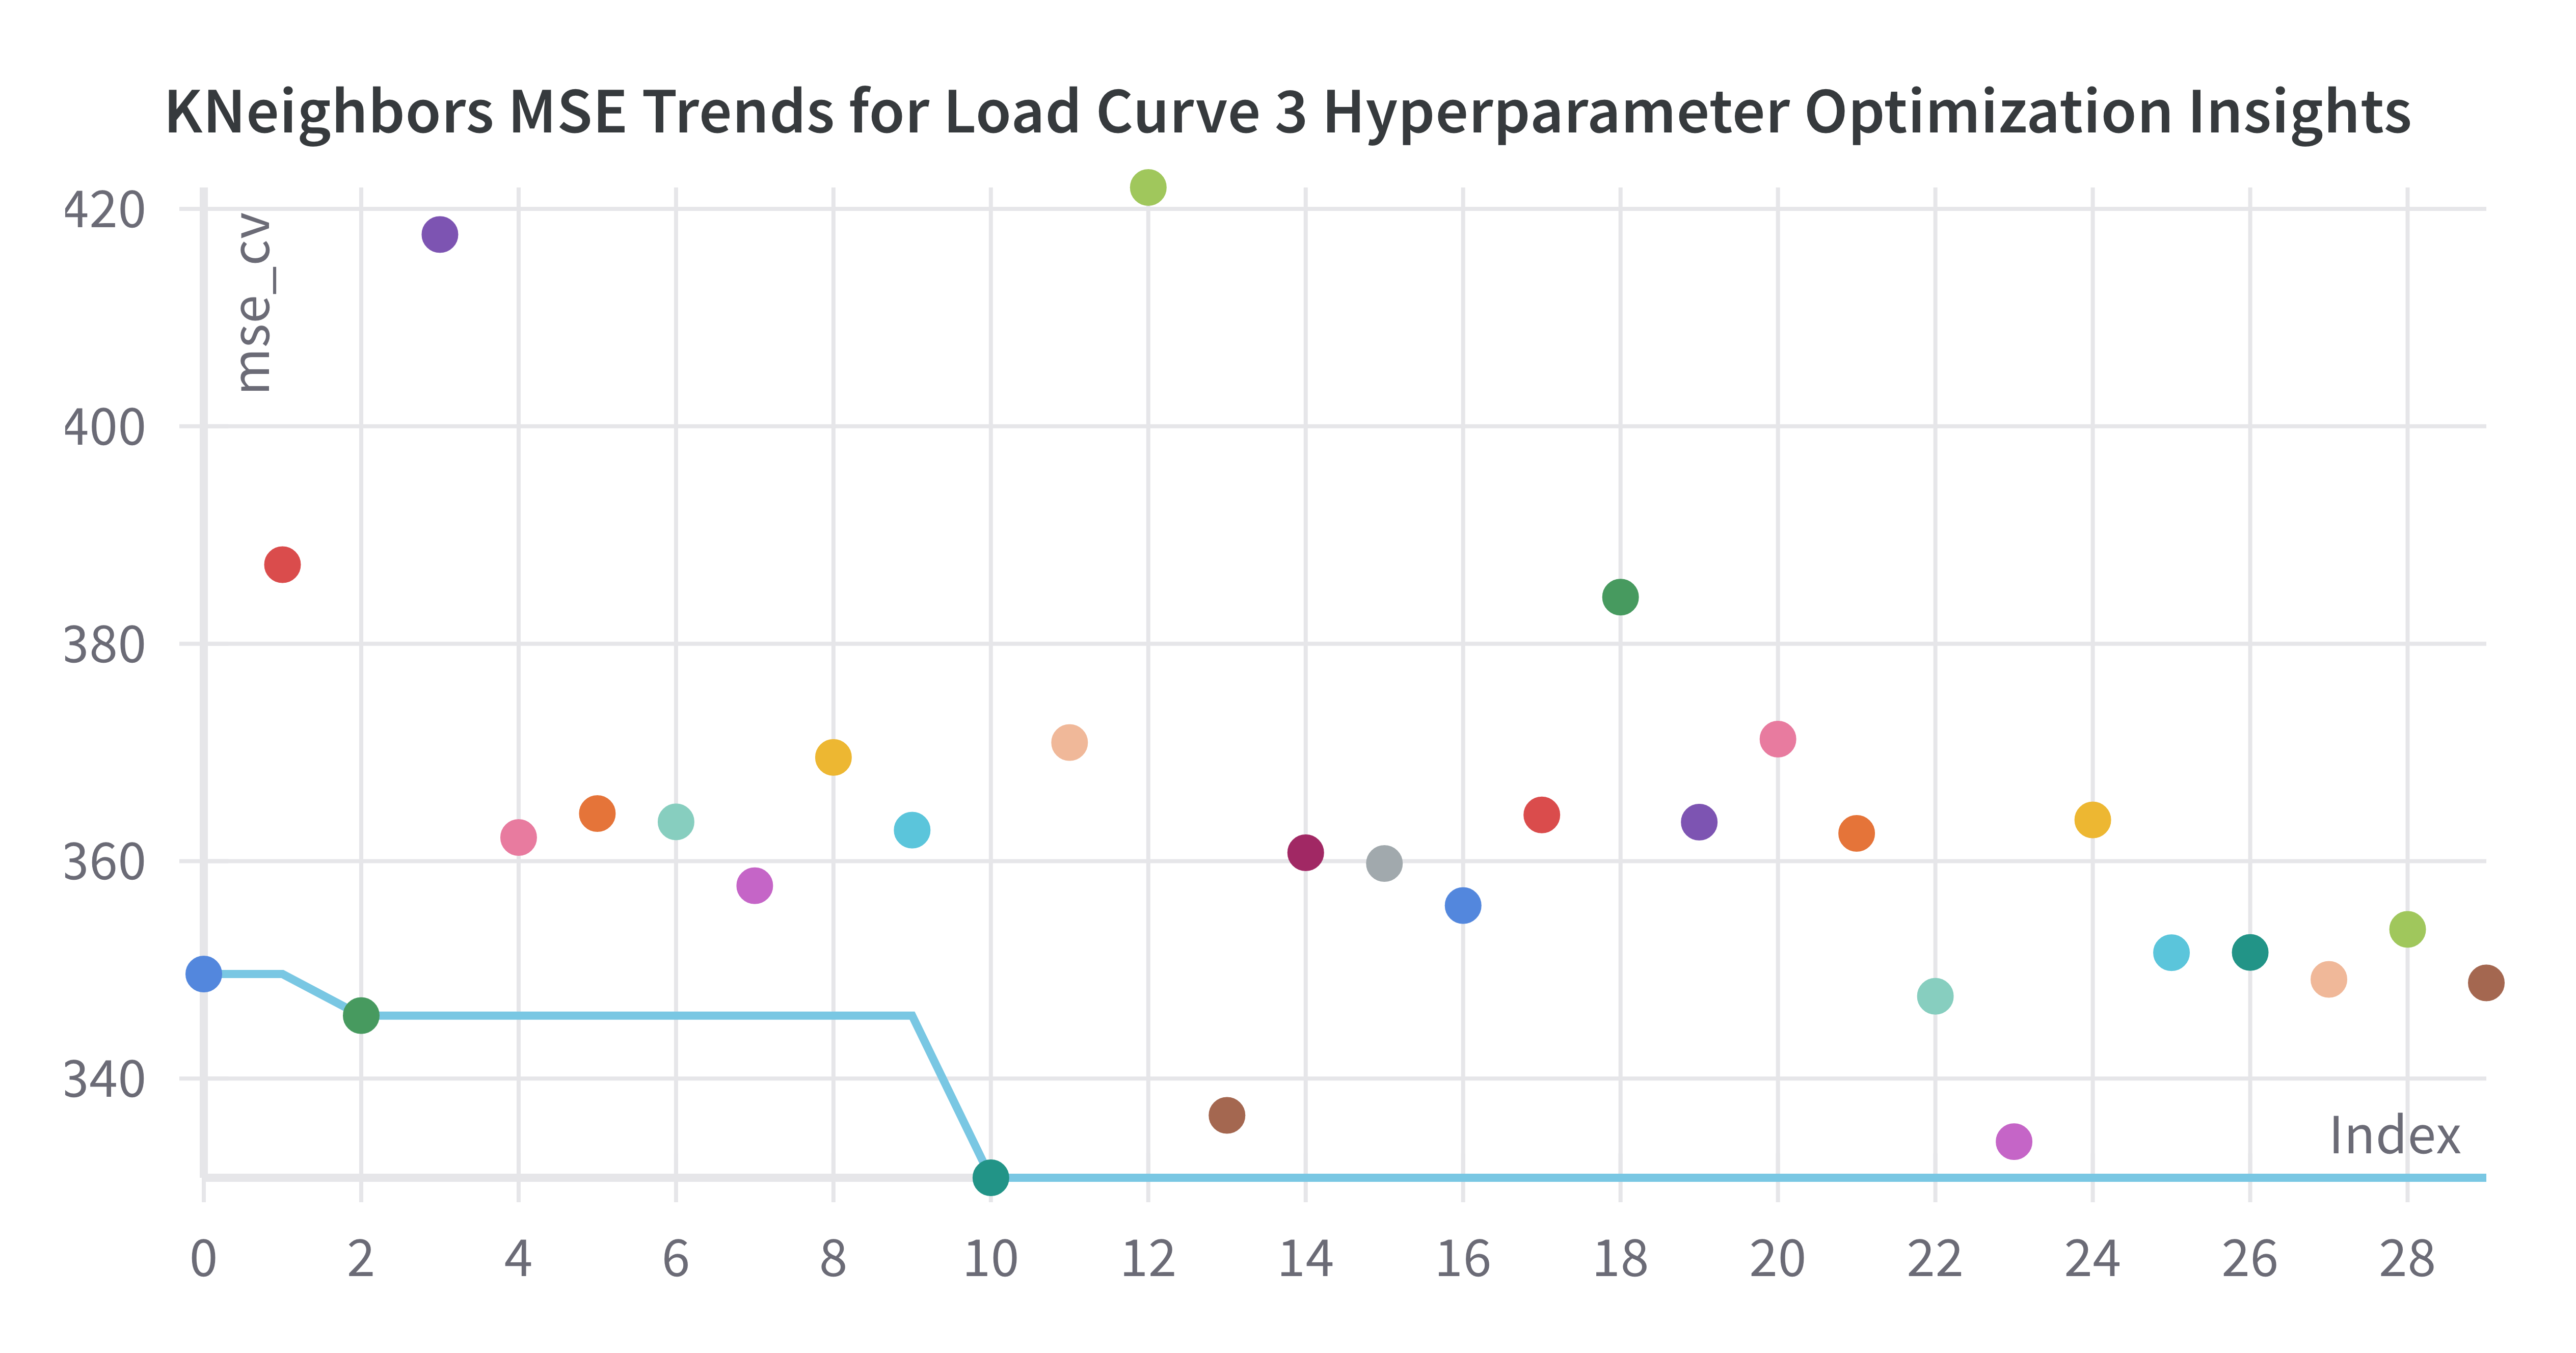
\includegraphics[width=0.75\textwidth]{ressources/Hyperparams/KNN/KNeighbors MSE Trends for Load Curve 3 Hyperparameter Optimization Insights.png}
    \caption{Bayesian hyperparameter optimization trends for KNN on Load Curve 3.}
    \label{fig:knn_lc3}
\end{figure}

\subsubsection{Final Model Results for KNN}
The performance evaluation of the KNN model on the three distinct load curves reveals significant disparities in predictive accuracy, casting doubt on the model's general applicability across varying datasets. Notably, the results for LC1 starkly underscore a concerning inadequacy in the model's fitting, contradicting expectations for high predictive performance.

For LC1, the KNN model reported an MSE of 3329.606, an MAE of 46.65, and an R2 of 0.699. These figures point to a problematic fit, where the model fails to capture the underlying patterns of the dataset effectively. The relatively low R2 value, far from indicating a near-perfect fit, rather highlights the model's struggle to accurately predict outcomes, suggesting a substantial discrepancy between observed and predicted values.

The results for LC2 and LC3, while showing improvement, still reflect only marginally acceptable levels of accuracy. LC2's performance, with an MSE of 42.83, an MAE of 5.239, and an R2 of 0.695, indicates a better fit than LC1 but still leaves much to be desired in terms of precision and reliability. The slight decrease in error metrics compared to LC1 does not necessarily signify a robust model performance, as the R2 value remains just below the threshold of generally accepted goodness-of-fit.

Similarly, LC3's outcomes, marked by an MSE of 299.634, an MAE of 13.391, and an R2 of 0.548, further validate concerns over the KNN model's diminishing accuracy across datasets with increasing complexity or volume. The notably lower R2 value underscores a weak correlation between the model's predictions and actual observations, highlighting a significant challenge in achieving dependable load forecasting with this model.

These findings compel a critical reassessment of the KNN model's utility for load forecasting tasks, especially in scenarios where data complexity and volume vary. The marked inconsistencies in model performance across LC1, LC2, and LC3 reveal that while KNN can offer some predictive capability, its effectiveness is critically dependent on dataset characteristics. Moreover, the particularly poor fit for LC1 and only marginally acceptable results for LC2 and LC3 raise questions about the suitability of KNN for complex pattern recognition tasks without significant model tuning or consideration of alternative, more sophisticated models.
\subsection{LSTM}
\subsubsection{Analysis of Bayesian Hyperparameter Optimization for LSTM}
The Bayesian hyperparameter optimization for the \gls*{LSTM} model applied to \gls*{LC1} did not yield successful results, as evidenced by the \gls*{MSE} trends. Despite the rigorous process of hyperparameter tuning, the \gls*{LSTM} model's performance on \gls*{LC1} was suboptimal, with high variance in the residuals and a final \gls*{MSE} score of 3731.48 on the test set. 

The best configuration for the \gls*{LSTM} model on \gls*{LC1} utilized a batch size of 256, a learning rate of 0.1, and enabled both daytime and day of the week indices. The dropout rate was set at 0.1 to mitigate overfitting, and the number of epochs was limited to 10, potentially to avoid extensive computational time. Despite these considerations, the high variance residuals test score of 18637.37 and a subpar R2 score of 0.6622 further confirm that the \gls*{LSTM} architecture was not adequate for capturing the dynamics of \gls*{LC1} effectively.

These outcomes indicate that for \gls*{LC1}, which may have nuanced temporal dependencies or non-linear relationships not captured by \gls*{LSTM}, alternative modeling techniques or additional feature engineering might be necessary to improve predictive performance.
Possibly due to additional external factors.

\begin{figure}[H]
    \centering
    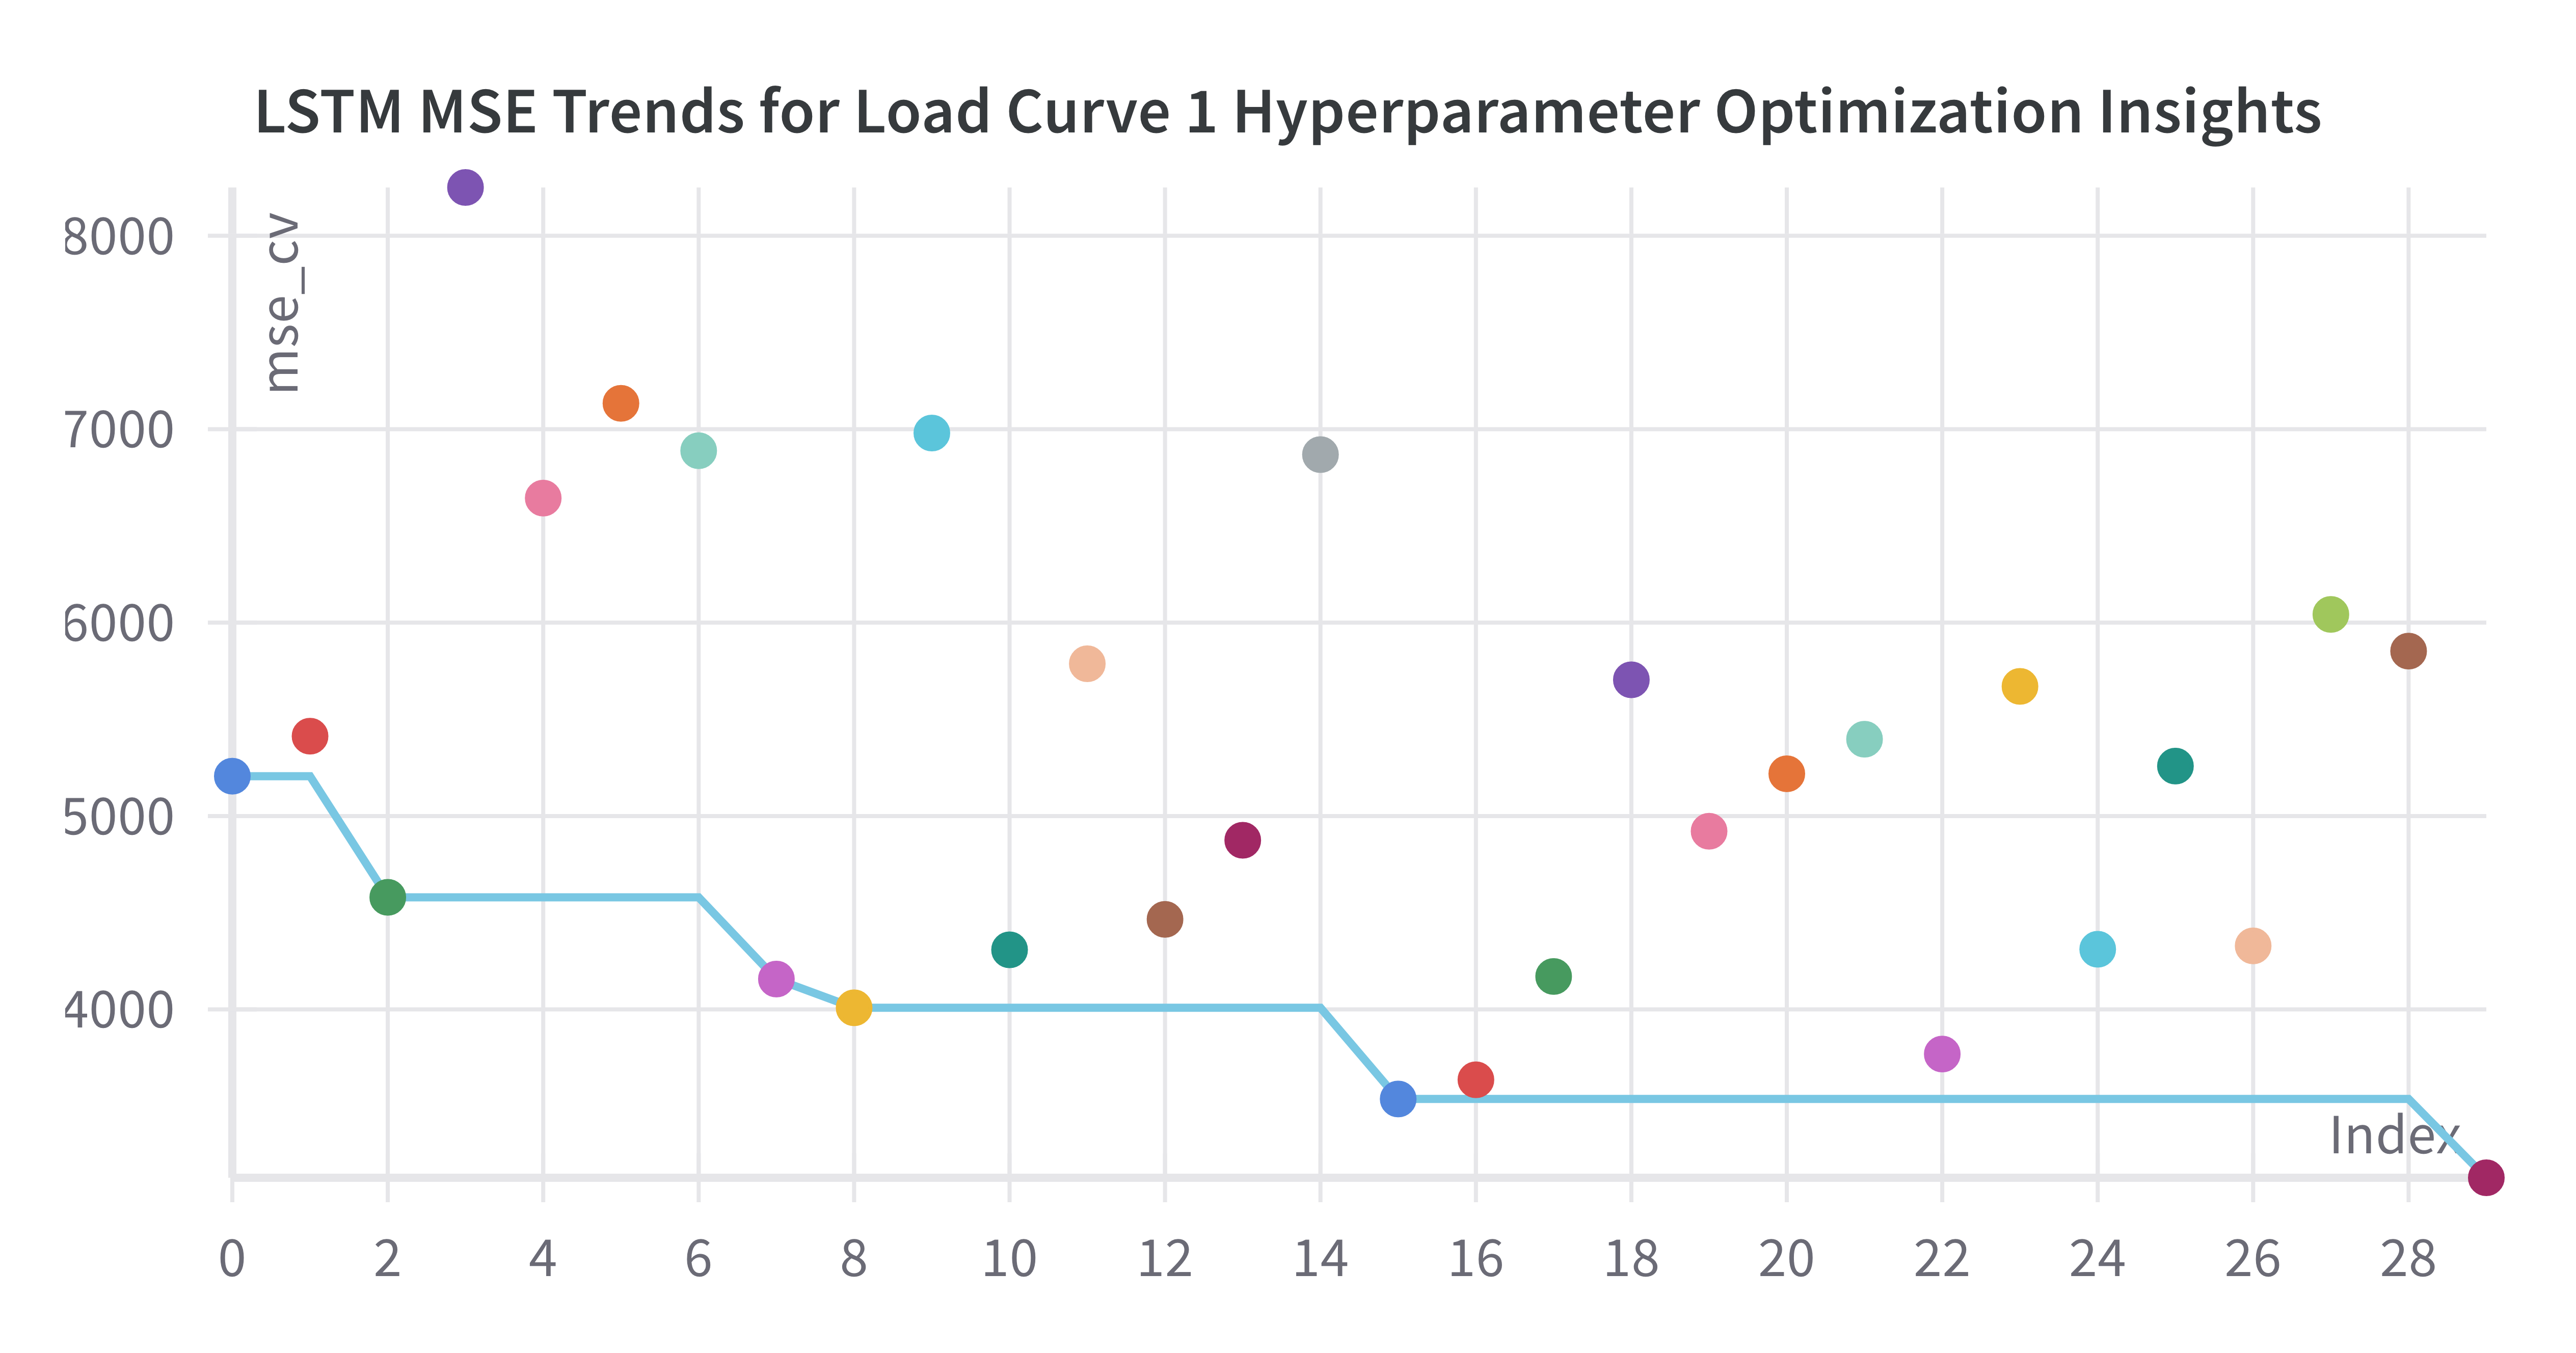
\includegraphics[width=0.75\textwidth]{ressources/Hyperparams/LSTM/LSTM MSE Trends for Load Curve 1 Hyperparameter Optimization Insights.png}
    \caption{Bayesian hyperparameter optimization trends for LSTM on Load Curve 1.}
    \label{fig:lstm_lc1}
\end{figure}
In the training phase for \gls*{LC2} and \gls*{LC3}, the LSTM model was subject to a restricted training regimen due to time constraints. Specifically, the model was trained using a 2-fold cross-validation approach and was limited to 10 runs. This reduced setup potentially affects the robustness of the hyperparameter optimization process and the generalizability of the resulting model. Typically, a larger number of folds and runs are preferred to ensure a more thorough exploration of the hyperparameter space and to mitigate the risk of overfitting to particular subsets of the data. Therefore, the outcomes of this training should be considered preliminary, and subsequent training with expanded folds and runs might be necessary to confirm these initial findings.
The Bayesian hyperparameter optimization for the \gls*{LSTM} model on \gls*{LC2} demonstrated significant improvements over \gls*{LC1}, yet the model failed to perform adequately. Despite the optimization process, the \gls*{LSTM} model's \gls*{MSE} trends on \gls*{LC2} highlight a challenge in capturing the underlying load patterns with considerable variability in the results.

The most notable hyperparameter with a direct correlation to the model performance was `dropout`, with a high importance score of 0.3705 and a strong positive correlation of 0.8445. This suggests that regularization played a crucial role in the model's ability to generalize from the training data to unseen data. However, the parameter `shifts`, with an importance score of 0.2797 and a negative correlation of -0.6641, indicated that the model was particularly sensitive to the sequence length, which aligns with the sequential nature of load forecasting.

Interestingly, the `batch\_size` parameter had an importance score of 0.1115 with a positive correlation of 0.5179, showing that larger batch sizes could potentially yield better performance, reflecting the balance between training stability and the model's convergence speed.


\begin{figure}[H]
    \centering
    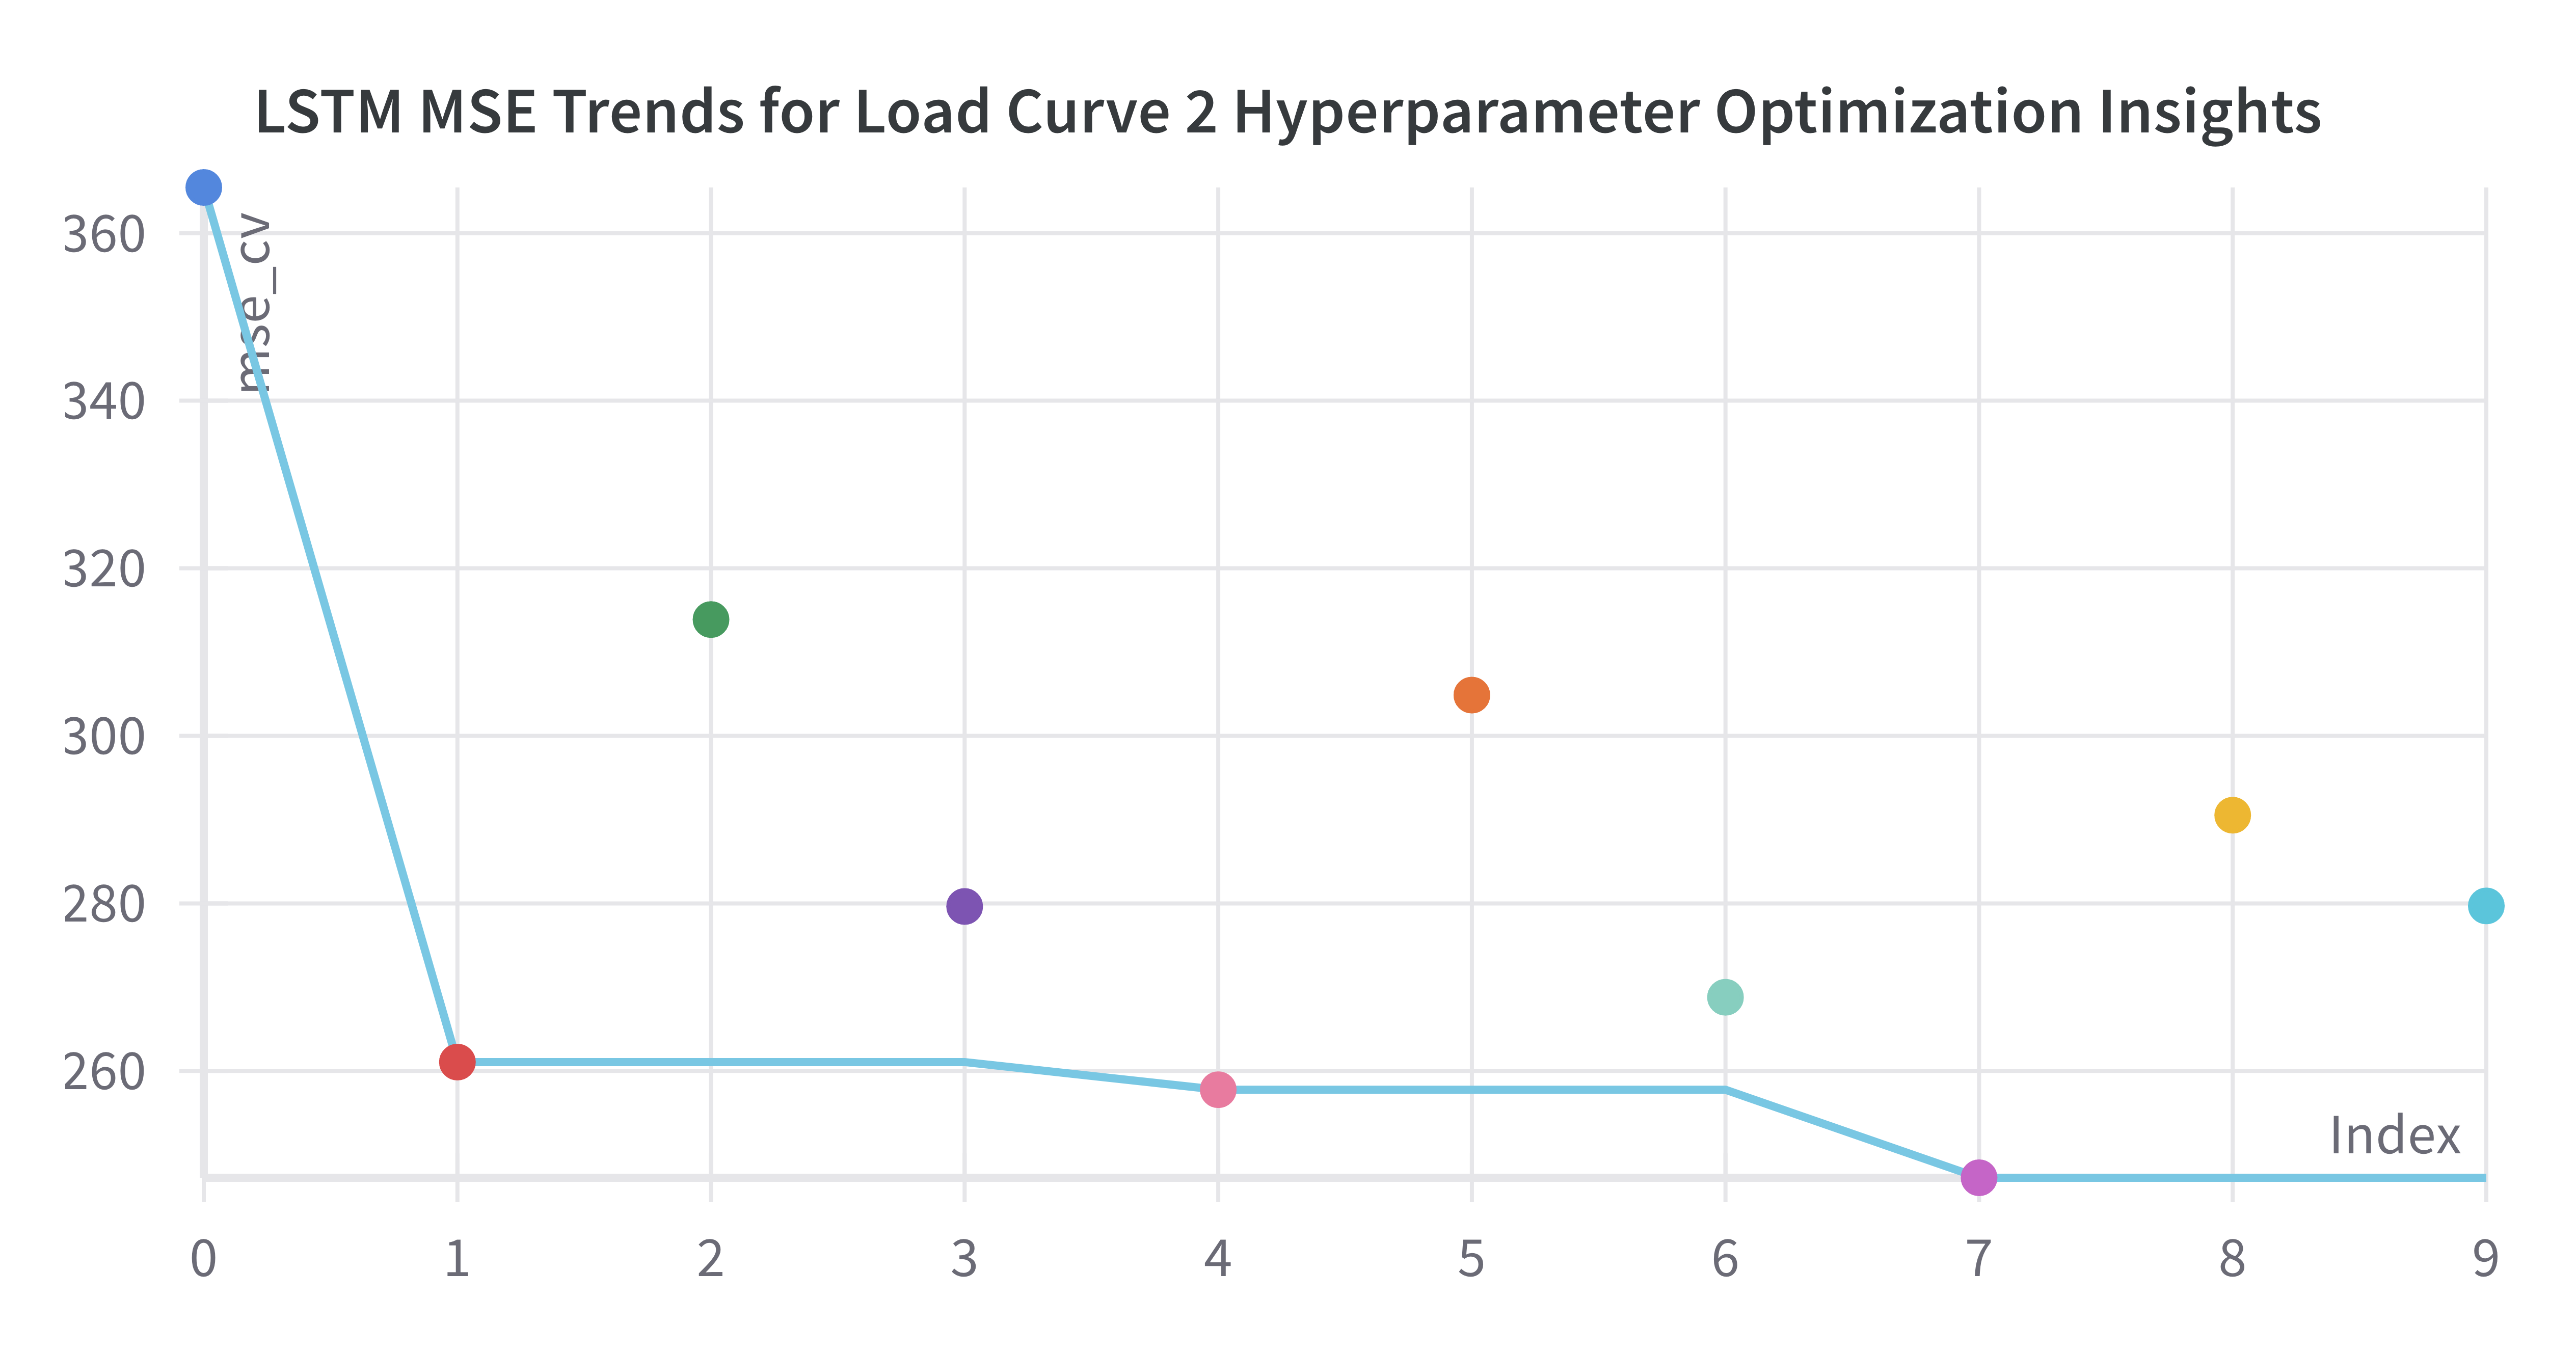
\includegraphics[width=0.75\textwidth]{ressources/Hyperparams/LSTM/LSTM MSE Trends for Load Curve 2 Hyperparameter Optimization Insights.png}
    \caption{Bayesian hyperparameter optimization trends for LSTM on Load Curve 2.}
    \label{fig:lstm_lc2}
\end{figure}
In the Bayesian hyperparameter optimization process for the \gls*{LSTM} model on Load Curve 3 (\gls*{LC3}), the model showed an improvement in \gls*{MSE} trends compared to \gls*{LC1}. However, despite these optimizations, the performance of \gls*{LSTM} on \gls*{LC3} was not optimal, suggesting that the model was not capturing the complexity of the data sufficiently.

The hyperparameter `epochs` showed a moderate importance score of 0.1915 with a negligible correlation, implying that increasing the number of training cycles did not significantly impact model performance. Meanwhile, `learning\_rate`, with an importance score of 0.2787 and a positive correlation of 0.4013, indicated that the speed at which the model learned had a substantial impact on its predictive accuracy. This emphasizes the delicate balance required in setting the learning rate for training deep learning models on time-series data.

The hyperparameters `dropout` and `batch\_size` also revealed interesting insights. `Dropout`, with an importance score of 0.097 and a positive correlation, hinted at its effectiveness in preventing overfitting. Conversely, the `batch\_size` had a negative correlation, suggesting that larger batch sizes might not always be beneficial, possibly due to the complex dynamics of the load curve data.

Despite these findings, the \gls*{LSTM}'s overall performance on \gls*{LC3} reflected the challenges inherent in modeling and predicting load data, which may necessitate a more sophisticated approach or additional feature engineering to improve accuracy.

\subsubsection{Final Model Results for LSTM}

The \gls*{LSTM} models showcased a spectrum of performance across the evaluated load curves. For \gls*{LC1}, the \gls*{LSTM} achieved a \gls*{R2} score of 0.662 on the test set, yet with a high \gls*{MSE} of 3731.49 and considerable variance in residuals of 18637.37, implying a decent model fit with overpredictions in certain instances. Contrastingly, \gls*{LC2} underperformed with a negative \gls*{R2} of -0.019 and lower \gls*{MSE} of 143.26, indicating potential overfitting or model inadequacy. \gls*{LC3} offered moderate predictive accuracy, with an \gls*{R2} of 0.402 and a lower variance in residuals, despite a \gls*{MSE} of 396.36. 
These results show that \gls*{LSTM} is not suitable for load prediction in this context.



 \subsection{Comparative Analysis of Predictive Performance Across all Models} 
 \subsection{Comparative Analysis of Predictive Performance Across all Models}

This comparative analysis delves into the strengths and weaknesses of four distinct predictive models: XGBoost, ARD, KNN, and LSTM, as applied to the task of forecasting load curves for industrial machinery. The evaluation is based on their performance across three datasets, encapsulated by metrics such as MSE, MAE, and the $R^2$.

\textbf{XGBoost }emerged as the standout model, demonstrating superior predictive accuracy across all three load curves. It not only achieved the lowest MSE and MAE but also the highest $R^2$ values, indicating a robust fit to the data. XGBoost's strength lies in its ensemble learning approach, effectively capturing complex non-linear relationships within the data. Moreover, its feature importance analysis revealed insightful patterns, affirming the model's ability to discern key predictors of load demand. However, the reliance on extensive parameter tuning to achieve optimal performance underscores the model's complexity and the need for computational resources.

\textbf{ARD }presented a mixed performance, with reasonable results on the second and third load curves but significantly underperforming on the first. The model's Bayesian framework allows for automatic feature relevance determination, which is a strength in identifying and focusing on significant predictors. However, its overall lower predictive accuracy compared to XGBoost highlights potential limitations in handling highly complex datasets or capturing intricate temporal dynamics.

KNN displayed moderate predictive accuracy, with performance metrics generally falling behind XGBoost but surpassing ARD in certain aspects. KNN's instance-based learning approach is advantageous for datasets with clear, localized patterns, but its performance deteriorates with increasing complexity and noise. The model's simplicity is a double-edged sword; while it ensures ease of understanding and implementation, it limits the ability to capture more sophisticated patterns without extensive feature engineering.

LSTM, despite its advanced capability to model sequential data and temporal dependencies, did not achieve competitive results in this context. The model's performance was particularly disappointing on the first load curve, with better but still suboptimal results on the others. LSTMs are theoretically well-suited for time-series forecasting; however, their effectiveness is highly contingent on the availability of large datasets and extensive tuning. The model's underperformance may also highlight challenges in feature selection and the need for more nuanced temporal feature engineering.

In conclusion, while \textbf{XGBoost} stands out for its high accuracy and adaptability, the analysis underscores the importance of matching model capabilities with the specific characteristics of the dataset. Each model presents unique strengths and potential drawbacks, with XGBoost offering the best balance of performance, complexity, and interpretability for this specific forecasting task. Future work could explore hybrid or ensemble methods that combine the strengths of these models, potentially leveraging LSTM's temporal modeling capabilities and XGBoost's robustness to further enhance predictive accuracy.

\begin{table}[H]
\centering
\caption{Comparison of Model Performance Metrics Across Load Curves. Best values are bold}
\label{tab:model_performance}
\begin{tabular}{@{\hspace{1em}}lccc}
\toprule
\textbf{Model} & \textbf{Load Curve 1} & \textbf{Load Curve 2} & \textbf{Load Curve 3} \\
\midrule
\multicolumn{4}{l}{\textbf{XGBoost}} \\
\midrule
MSE &\textbf{ 453.107} & \textbf{11.090} & \textbf{67.493} \\
MAE & \textbf{15.756} & \textbf{2.600} & \textbf{7.091} \\
$R^2$ & \textbf{0.959} & \textbf{0.921} &\textbf{ 0.898} \\
\midrule
\multicolumn{4}{l}{\textbf{ARD}} \\
\midrule
MSE & 6184.419 & 34.239 & 253.466 \\
MAE & 63.358 & 4.644 & 12.792 \\
$R^2$ & 0.44 & 0.757 & 0.618 \\
\midrule
\multicolumn{4}{l}{\textbf{KNN}} \\
\midrule
MSE & 3329.606 & 42.83 & 299.634 \\
MAE & 46.65 & 5.239 & 13.391 \\
$R^2$ & 0.699 & 0.695 & 0.548 \\
\midrule
\multicolumn{4}{l}{\textbf{LSTM}} \\
\midrule
MSE & 3731.486 & 143.257 & 536.67 \\
MAE & 39.185 & 9.806 & 19.496 \\
$R^2$ & 0.6623 & -0.01869 & 0.19 \\
\bottomrule
\end{tabular}
\end{table}


\section{Conclusion}
In conclusion, our objective was to develop a precise and adaptable forecasting model to predict load curves for Siemens machinery, aiding in determining energy requirements. Upon analyzing the dataset, identified as a regression problem, we employed \gls*{LSTM}, \gls*{ARD}, \gls*{KNN}, and \gls*{xgboost}. We trained the data of the first generation and checked the results for the smallest \gls*{MSE}. \gls*{LSTM}, despite its reputation, yielded unsatisfactory results due to model complexity; regularization did not mitigate this issue. Limited data availability may have hindered \gls*{LSTM}'s effectiveness, a potential consequence of regulatory constraints. Conversely, \gls*{xgboost} demonstrated superior performance. 

Focusing on \gls*{xgboost}, we expanded feature sets significantly. Bayesian hyperparameter training substantially enhanced model performance, underscoring \gls*{xgboost}'s efficacy. Notably, \gls*{xgboost} exhibited optimal model capacity for a relatively modest dataset size, contrasting with image datasets. Furthermore, through extensive training, we rectified initial shortcomings in peak prediction accuracy. Feature importance analysis revealed radiation to be inconsequential, affirming the validity of our selected features in enhancing model efficacy. In summary, \gls*{xgboost} emerges as a robust solution, delivering exceptional results with minimal data. Our findings underscore the importance of feature selection and hyperparameter tuning in optimizing model performance for load curve prediction in Siemens machinery. 

Future research could address the topic of making our model more robust with methods such as stacking or boosting in combination with \gls*{xgboost}. Adding sensors to capture more real-time operational data could further enhance the accuracy and timeliness of the load curve predictions. Explainable AI techniques could give further insights into the decision-making process of our model.

\subsubsection*{Acknowledgments}
We would like to thank Siemens AG for their cooperation in this research project. Their willingness to provide us with the necessary load data was of decisive importance for the progress of our project.


\bibliography{iclr2021_conference}
\bibliographystyle{iclr2021_conference}

\appendix
\section{Appendix}
You may include other additional sections here.

\end{document}
